\documentclass{article}
\usepackage{amsfonts} % For open face letters
\usepackage{amsmath} % For align*
\usepackage{bookmark} % For links
\usepackage{graphicx} % For images
\usepackage{enumitem} % For customisable list labels
\usepackage{siunitx} % For units

\graphicspath{{./images/}}
\hypersetup{
  colorlinks=true,
  linkcolor=blue,
  urlcolor=blue
}

\DeclareMathOperator{\arcosh}{arcosh}
\DeclareMathOperator{\csch}{csch}
\DeclareSIUnit\angstrom{\text{Å}}

\renewcommand{\Re}{\operatorname{Re}}
\renewcommand{\vec}[1]{\boldsymbol{\mathbf{#1}}}
\newcommand{\dvec}[1]{\dot{\vec{#1}}}
\newcommand{\ddvec}[1]{\ddot{\vec{#1}}}
\newcommand{\tvec}[1]{\tilde{\vec{#1}}}
\newcommand{\uvec}[1]{\hat{\vec{#1}}}

\newcommand{\ke}{\frac{1}{4 \pi \epsilon_0}}

\def\rcurs{{\mbox{$\resizebox{.09in}{.08in}{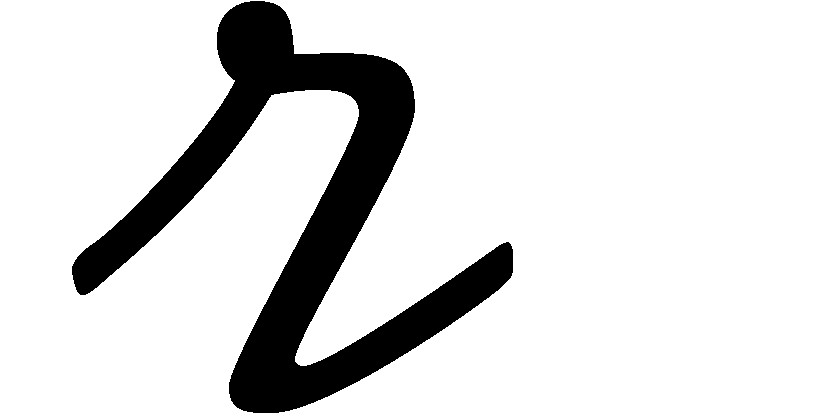
\includegraphics[trim= 1em 0 14em 0,clip]{ScriptR}}$}}}
\def\brcurs{{\mbox{$\resizebox{.09in}{.08in}{
\includegraphics[trim= 1em 0 14em 0,clip]{BoldR}}$}}}
\def\hrcurs{{\mbox{$\hat \brcurs$}}}

\setlist[enumerate, 1]{label={(\alph*)}}
\setlist[enumerate, 2]{label={(\roman*)}}

\title{Introduction to Electrodynamics by David J. Griffiths Problems}
\author{Chris Doble}
\date{December 2023}

\begin{document}

\maketitle

\tableofcontents

\setcounter{section}{1}
\section{Electrostatics}

\subsection{}

\begin{enumerate}
  \item $\vec{0}$

  \item The same as if only the opposite charge were present — all others are cancelled out.
\end{enumerate}

\subsection{}

\begin{align*}
  \vec{E} & = \ke 2 \frac{q}{\rcurs^2} \cos \theta \uvec{x}      \\
          & = \ke \frac{d q}{[(d / 2)^2 + z^2]^{3 / 2}} \uvec{x}
\end{align*}

\subsection{}

\begin{align*}
  \vec{r}  & = z \uvec{z}                                                                                                                          \\
  \vec{r}' & = x \uvec{x}                                                                                                                          \\
  \brcurs  & = z \uvec{z} - x \uvec{x}                                                                                                             \\
  \rcurs   & = \sqrt{x^2 + z^2}                                                                                                                    \\
  \hrcurs  & = \frac{z \uvec{z} - x \uvec{x}}{\sqrt{x^2 + z^2}}                                                                                    \\
  \vec{E}  & = \ke \int_0^L \frac{\lambda}{x^2 + z^2} \frac{z \uvec{z} - x \uvec{x}}{\sqrt{x^2 + z^2}} \,d x                                       \\
           & = \ke \lambda \left( z \uvec{z} \int_0^L \frac{1}{(x^2 + z^2)^{3 / 2}} \,d x - \uvec{x} \int_0^L \frac{x}{(x^2 + z^2)} \,d x \right)  \\
           & = \ke \lambda \left[ \frac{L}{z \sqrt{L^2 + z^2}} \uvec{z} - \left( \frac{1}{z} - \frac{1}{\sqrt{L^2 + z^2}} \right) \uvec{x} \right] \\
           & = \ke \frac{\lambda}{z} \left[ \left( -1 + \frac{z}{\sqrt{L^2 + z^2}} \right) \uvec{x} + \frac{L}{\sqrt{L^2 + z^2}} \uvec{z} \right]
\end{align*}

\subsection{}

The electric field a distance $z$ above the midpoint of a line segment of length $2 L$ and uniform line charge $\lambda$ is \[\vec{E} = \ke \frac{2 \lambda L}{z \sqrt{z^2 + L^2}} \uvec{z}.\]

Applying this to the four sides of the square, the horizontal components of opposite sides cancel leaving only the vertical component.

\begin{align*}
  \cos \theta & = \frac{z}{\rcurs}                                                                                                      \\
              & = \frac{z}{\sqrt{(a / 2)^2 + z^2}}                                                                                      \\
  \vec{E}     & = 4 \left( \ke \frac{\lambda a}{\sqrt{(a / 2)^2 + z^2} \sqrt{(a / 2)^2 + (a / 2)^2 + z^2}} \uvec{z} \right) \cos \theta \\
              & = \ke \frac{4 a \lambda z}{[(a / 2)^2 + z^2] \sqrt{(a^2 / 2) + z^2}} \uvec{z}
\end{align*}

\subsection{}

\begin{align*}
  \vec{E} & = \ke \int_0^{2 \pi} \frac{\lambda r}{r^2 + z^2} \cos \alpha \,d \theta \,\uvec{z} \\
          & = \ke \frac{2 \pi \lambda r z}{(r^2 + z^2)^{3 / 2}} \uvec{z}
\end{align*}

\subsection{}

\begin{align*}
  \vec{E} & = \ke \int \frac{d q}{\rcurs^2} \cos \theta \uvec{z}                                                          \\
          & = \ke \int_0^{2 \pi} \int_0^R \frac{\sigma}{r^2 + z^2} \frac{z}{\sqrt{r^2 + z^2}} r \,d r \,d \theta \uvec{z} \\
          & = \ke 2 \pi \sigma z \int_0^R \frac{r}{(r^2 + z^2)^{3 / 2}} \,d r \,\uvec{z}                                  \\
          & = \ke 2 \pi \sigma z \left( \frac{1}{z} - \frac{1}{\sqrt{R^2 + z^2}} \right) \uvec{z}
\end{align*}

When $R \rightarrow \infty$ \[\vec{E} = \frac{\sigma}{2 \epsilon_0} \uvec{z}.\]

\subsection{}

\[\vec{E} = \begin{cases}
    \ke \frac{q}{z^2} \uvec{z} & z > R \\
    \vec{0}                    & z < R
  \end{cases}\]

\subsection{}

\[\vec{E} = \begin{cases}
    \ke \frac{q}{z^2} \uvec{z}   & z > R \\
    \ke \frac{q z}{R^3} \uvec{z} & z < R
  \end{cases}\]

\subsection{}

\begin{enumerate}
  \item

        \begin{align*}
          \rho & = \epsilon_0 \nabla \cdot \vec{E}                              \\
               & = \epsilon_0 \frac{1}{r^2} \frac{\partial}{\partial r} (k r^5) \\
               & = 5 \epsilon_0 k r^2
        \end{align*}

  \item

        \begin{align*}
          Q_\text{enc} & = \epsilon_0 \oint \vec{E} \cdot d \vec{a}                                                        \\
                       & = \epsilon_0 \int_0^{2 \pi} \int_0^\pi k R^3 R \,d \theta R \sin \theta \,d \phi                  \\
                       & = 2 \pi \epsilon_0 k R^5 [-\cos \theta]_0^\pi                                                     \\
                       & = 4 \pi \epsilon_0 k R^5                                                                          \\
          Q_\text{enc} & = \int_V \rho \,d \tau                                                                            \\
                       & = \int_0^{2 \pi} \int_0^\pi \int_0^R 5 \epsilon_0 k r^2 \,d r r \,d \theta r \sin \theta \,d \phi \\
                       & = 10 \pi \epsilon_0 k \int_0^\pi \int_0^R r^4 \sin \theta \,d r \,d \theta                        \\
                       & = 2 \pi \epsilon_0 k R^5 [-\cos \theta]_0^\pi                                                     \\
                       & = 4 \pi \epsilon_0 k R^5
        \end{align*}
\end{enumerate}

\subsection{}

If the charge was surrounded by $8$ such cubes the total flux through all the cubes would be $q / \epsilon_0$. There are $24$ outside faces to the larger cube, so the total flux through the shaded face is $q / (24 \epsilon_0)$.

\subsection{}

\begin{align*}
  \int \vec{E}_\text{inside} \cdot d \vec{a}  & = \frac{Q_\text{enc}}{\epsilon_0}     \\
                                              & = 0                                   \\
  \vec{E}_\text{inside}                       & = \vec{0}                             \\
  \int \vec{E}_\text{outside} \cdot d \vec{a} & = \frac{Q_\text{enc}}{\epsilon_0}     \\
  4 \pi r^2 E_\text{outside}                  & = \frac{4 \pi R^2 \sigma}{\epsilon_0} \\
  \vec{E}_\text{outside}                      & = \ke \frac{q}{r^2} \uvec{r}
\end{align*}

\subsection{}

\begin{align*}
  \int \vec{E} \cdot d \vec{a} & = \frac{Q_\text{enc}}{\epsilon_0}             \\
  4 \pi r^2 E                  & = \frac{\frac{4}{3} \pi r^3 \rho}{\epsilon_0} \\
  \vec{E}                      & = \frac{r \rho}{3 \epsilon_0} \uvec{r}
\end{align*}

\subsection{}

\begin{align*}
  \int \vec{E} \cdot d \vec{a} & = \frac{Q_\text{enc}}{\epsilon_0}                       \\
  2 \pi s l E                  & = \frac{l \lambda}{\epsilon_0}                          \\
  \vec{E}                      & = \frac{1}{2 \pi \epsilon_0} \frac{\lambda}{s} \uvec{s}
\end{align*}

\subsection{}

\begin{align*}
  Q_\text{enc}                 & = \int_V \rho \,d \tau                                                             \\
                               & = \int_0^{2 \pi} \int_0^\pi \int_0^r k r'^3 \sin \theta \,d r' \,d \theta \,d \phi \\
                               & = 2 \pi k \int_0^\pi \left[ \frac{1}{4} r'^4 \sin \theta \right]_0^r \,d \theta    \\
                               & = \frac{1}{2} \pi k r^4 [-\cos \theta]_0^\pi                                       \\
                               & = \pi k r^4                                                                        \\
  \int \vec{E} \cdot d \vec{a} & = \frac{Q_\text{enc}}{\epsilon_0}                                                  \\
  4 \pi r^2 E                  & = \frac{\pi k r^4}{\epsilon_0}                                                     \\
  \vec{E}                      & = \frac{k r^2}{4 \epsilon_0} \uvec{r}
\end{align*}

\subsection{}

\begin{enumerate}
  \item $\vec{E} = \vec{0}$

  \item

        \begin{align*}
          Q_\text{enc} & = \int_0^{2 \pi} \int_0^\pi \int_a^r k \sin \theta \,d r' \,d \theta \,d \phi \\
                       & = 4 \pi k (r - a)                                                             \\
          4 \pi r^2 E  & = \frac{4 \pi k (r - a)}{\epsilon_0}                                          \\
          \vec{E}      & = \frac{k (r - a)}{\epsilon_0 r^2} \uvec{r}
        \end{align*}

  \item $\vec{E} = \frac{k (b - a)}{\epsilon_0 r^2} \uvec{r}$
\end{enumerate}

\subsection{}

\begin{enumerate}
  \item

        \begin{align*}
          Q_\text{enc} & = \pi s^2 l \rho                       \\
          2 \pi s l E  & = \frac{\pi s^2 l \rho}{\epsilon_0}    \\
          \vec{E}      & = \frac{s \rho}{2 \epsilon_0} \uvec{s}
        \end{align*}

  \item \[\vec{E} = \frac{a^2 \rho}{2 \epsilon_0 s} \uvec{s}\]

  \item \[\vec{E} = \vec{0}\]
\end{enumerate}

\subsection{}

\begin{align*}
  2 A E_\text{inside}   & = \frac{2 A y \rho}{\epsilon_0}           \\
  \vec{E}_\text{inside} & = \frac{y \rho}{\epsilon_0}               \\
  \vec{E}               & = \begin{cases}
                              \frac{d \rho}{\epsilon_0}  & d < y      \\
                              \frac{y \rho}{\epsilon_0}  & 0 < y < d  \\
                              -\frac{y \rho}{\epsilon_0} & -d < y < 0 \\
                              -\frac{d \rho}{\epsilon_0} & y < -d
                            \end{cases}
\end{align*}

\subsection{}

The electric field inside a uniformly charged solid sphere is \[\vec{E} = \frac{r \rho}{3 \epsilon_0} \uvec{r}.\]

\begin{align*}
  \vec{d} & = \vec{r}_1 - \vec{r}_2                                                               \\
  \vec{E} & = \frac{r_1 \rho}{3 \epsilon_0} \uvec{r}_1 - \frac{r_2 \rho}{3 \epsilon_0} \uvec{r}_2 \\
          & = \frac{\rho}{3 \epsilon_0} (\vec{r}_1 - \vec{r}_2)                                   \\
          & = \frac{\rho}{3 \epsilon_0} \vec{d}
\end{align*}

\setcounter{subsection}{19}
\subsection{}

a is impossible because its curl is nonzero.

\begin{align*}
  V         & = -\int_0^y 2 k x y' \,d y' - \int_0^z 2 k y z' \,d z                                    \\
            & = -2 k x \left[ \frac{1}{2} y'^2 \right]_0^y - 2 k y \left[ \frac{1}{2} z'^2 \right]_0^z \\
            & = -k (x y^2 + y z^2)                                                                     \\
  -\nabla V & = k [y^2 \uvec{x} + (2 x y + z^2) \uvec{y} + 2 y z \uvec{z}]                             \\
            & = \vec{E}
\end{align*}

\subsection{}

\begin{align*}
  \vec{E}                  & = \begin{cases}
                                 \ke \frac{q}{r^2}   & r > R \\
                                 \ke \frac{q r}{R^3} & r < R
                               \end{cases}                                                                    \\
  V_\text{outside}(r)      & = -\int_\infty^r \ke \frac{q}{r'^2} \,d r'                                                       \\
                           & = -\ke q \left[ -\frac{1}{r'} \right]_\infty^r                                                   \\
                           & = \ke \frac{q}{r}                                                                                \\
  -\nabla V_\text{outside} & = \ke \frac{q}{r^2} \uvec{r}                                                                     \\
                           & = \vec{E}_\text{outside}                                                                         \\
  V_\text{inside}(r)       & = -\left( \int_\infty^R \ke \frac{q}{r'^2} \,d r' + \int_R^r \ke \frac{q r'}{R^3} \,d r' \right) \\
                           & = -\left( -\ke \frac{q}{R} + \ke \frac{q}{R^3} \left[ \frac{1}{2} r'^2 \right]_R^r \right)       \\
                           & = \ke \frac{q}{2 R} \left[ 3 - \left( \frac{r}{R} \right)^2 \right]                              \\
  -\nabla V_\text{inside}  & = \ke \frac{q r}{R^3} \uvec{r}                                                                   \\
                           & = \vec{E}_\text{inside}
\end{align*}

\subsection{}

\begin{align*}
  \vec{E}   & = \frac{1}{2 \pi \epsilon_0} \frac{\lambda}{s} \uvec{s}          \\
  V         & = -\int_O^s \frac{1}{2 \pi \epsilon_0} \frac{\lambda}{s'} \,d s' \\
            & = -\frac{1}{2 \pi \epsilon_0} \lambda \ln \frac{s}{O}            \\
  -\nabla V & = \frac{1}{2 \pi \epsilon_0} \frac{\lambda}{s} \uvec{s}
\end{align*}

\subsection{}

\begin{align*}
  \vec{E} & = \begin{cases}
                \vec{0}                                   & r < a     \\
                \frac{k (r - a)}{\epsilon_0 r^2} \uvec{r} & a < r < b \\
                \frac{k (b - a)}{\epsilon_0 r^2} \uvec{r} & b < r
              \end{cases}                                                                                           \\
  V(0)    & = -\int_\infty^0 E \,d r                                                                                                                          \\
          & = -\left( \int_\infty^b \frac{k (b - a)}{\epsilon_0 r^2} \,d r + \int_b^a \frac{k (r - a)}{\epsilon_0 r^2} \,d r \right)                          \\
          & = -\left( \frac{k (b - a)}{\epsilon_0} \left[ -\frac{1}{r} \right]_\infty^b + \frac{k}{\epsilon_0} \left[ \ln r + \frac{a}{r} \right]_b^a \right) \\
          & = -\left[ -\frac{k (b - a)}{\epsilon_0 b} + \frac{k}{\epsilon_0} \left( \ln a + 1 - \ln b - \frac{a}{b} \right) \right]                           \\
          & = -\frac{k}{\epsilon_0} \left( -1 + \frac{a}{b} + \ln \frac{a}{b} + 1 - \frac{a}{b} \right)                                                       \\
          & = \frac{k}{\epsilon_0} \ln \frac{b}{a}
\end{align*}

\subsection{}

\begin{align*}
  V(b) - V(0) & = -\int_0^b E \,d r                                                                                                            \\
              & = -\left( \int_0^a \frac{s \rho}{2 \epsilon_0} \,d s + \int_a^b \frac{a^2 \rho}{2 \epsilon_0 s} \,d s \right)                  \\
              & = -\left( \frac{\rho}{2 \epsilon_0} \left[ \frac{1}{2} s^2 \right]_0^a + \frac{a^2 \rho}{2 \epsilon_0} \ln \frac{b}{a} \right) \\
              & = -\left( \frac{a^2 \rho}{4 \epsilon_0} + \frac{a^2 \rho}{2 \epsilon_0} \ln \frac{b}{a} \right)                                \\
              & = -\frac{a^2 \rho}{4 \epsilon_0} \left( 1 + 2 \ln \frac{a}{b} \right)
\end{align*}

\subsection{}

\begin{enumerate}
  \item \[V = \ke \frac{2 q}{\sqrt{(d / 2)^2 + z^2}}\]

  \item

        \begin{align*}
          V & = \ke \int_{-L}^L \frac{\lambda}{\sqrt{x^2 + z^2}} \,d x                    \\
            & = \ke \lambda \ln \left( 1 + \frac{2 L (L + \sqrt{L^2 + z^2})}{z^2} \right)
        \end{align*}

  \item

        \begin{align*}
          V & = \ke \int_0^{2 \pi} \int_0^R \frac{\sigma}{\sqrt{r^2 + z^2}} r \,d r \,d \theta \\
            & = \ke 2 \pi \sigma (\sqrt{R^2 + z^2} - z)
        \end{align*}
\end{enumerate}

\subsection{}

\begin{align*}
  V_\text{bottom}                & = \ke \int_0^{2 \pi} \int_0^h \frac{\sqrt{2} \sigma z}{\sqrt{2} z} \,d \phi \,d z             \\
                                 & = \frac{\sigma h}{2 \epsilon_0}                                                               \\
  V_\text{top}                   & = \ke \int_0^{2 \pi} \int_0^h \frac{\sqrt{2} \sigma z}{\sqrt{z^2 + (h - z)^2}} \,d \phi \,d z \\
                                 & = \frac{\sqrt{2} \sigma}{2 \epsilon_0} \int_0^h \frac{z}{\sqrt{z^2 + (h - z)^2}} \,d z        \\
                                 & = \frac{\sigma h}{4 \epsilon_0} \ln (3 + 2 \sqrt{2})                                          \\
  V_\text{bottom} - V_\text{top} & = \frac{\sigma h}{2 \epsilon_0} \left[ 1 - \frac{1}{2} \ln (3 + 2 \sqrt{2}) \right]           \\
\end{align*}

\setcounter{subsection}{27}
\subsection{}

\begin{align*}
  V(r) & = \ke \int_0^{2 \pi} \int_0^\pi \int_0^R \frac{\rho r'^2 \sin \theta}{\sqrt{r^2 + r'^2 - 2 r r' \cos \theta}} \,d r' \,d \theta \,d \phi \\
       & = \frac{\rho}{2 \epsilon_0} \int_0^\pi \int_0^R \frac{r'^2 \sin \theta}{\sqrt{r^2 + r'^2 - 2 r r' \cos \theta}} \,d r' \,d \theta        \\
       & = \frac{\rho}{2 \epsilon_0} \left( R^2 - \frac{r^2}{3} \right)                                                                           \\
       & = \frac{q}{8 \pi \epsilon_0 R} \left( 3 - \frac{r^2}{R^2} \right)
\end{align*}

\setcounter{subsection}{30}
\subsection{}

\begin{enumerate}
  \item \[W = \frac{q^2}{4 \pi \epsilon_0 a} \left( \frac{1}{\sqrt{2}} - 2 \right)\]

  \item

        \begin{align*}
          W & = \ke \left( -\frac{q^2}{a} + \frac{q^2}{\sqrt{2} a} - \frac{q^2}{a} - \frac{q^2}{a} + \frac{q^2}{\sqrt{2} a} - \frac{q^2}{a} \right) \\
            & = \frac{q^2}{2 \pi \epsilon_0 a} \left( \frac{1}{\sqrt{2}} - 2 \right)
        \end{align*}
\end{enumerate}

\subsection{}

\begin{align*}
  % Conservation of energy
  W                                            & = \ke \frac{q_A q_B}{a}                                                           \\
  W                                            & = K_1 + K_2                                                                       \\
  \ke \frac{q_A q_B}{a}                        & = \frac{1}{2} m_A v_A^2 + \frac{1}{2} m_B v_B^2                                   \\
  \frac{1}{2 \pi \epsilon_0} \frac{q_A q_B}{a} & = m_A v_A^2 + m_B v_B^2                                                           \\
  % Conservation of momentum
  0                                            & = m_B v_B - m_A v_A                                                               \\
  v_B                                          & = \frac{m_A}{m_B} v_A                                                             \\
  \frac{1}{2 \pi \epsilon_0} \frac{q_A q_B}{a} & = m_A v_A^2 + m_B \left( \frac{m_A}{m_B} v_A \right)^2                            \\
                                               & = m_A v_A^2 + \frac{m_A^2}{m_B} v_A^2                                             \\
                                               & = \frac{m_A (m_A + m_B)}{m_B} v_A^2                                               \\
  v_A                                          & = \sqrt{\frac{1}{2 \pi \epsilon_0} \frac{q_A q_B}{(m_A + m_B) a} \frac{m_B}{m_A}} \\
  v_B                                          & = \sqrt{\frac{1}{2 \pi \epsilon_0} \frac{q_A q_B}{(m_A + m_B) a} \frac{m_A}{m_B}}
\end{align*}

\subsection{}

\begin{align*}
  W & = \ke \left( -\frac{q^2}{a} + \frac{q^2}{2 a} - \frac{q^2}{3 a} + \ldots \right) \\
    & = \ke \frac{q^2}{a} \sum_{n = 1}^\infty \frac{(-1)^n}{n}                         \\
    & = -\ke \frac{q^2}{a} \ln 2
\end{align*}

\subsection{}

\begin{enumerate}
  \item

        \begin{align*}
          V & = \begin{cases}
                  \ke \frac{q}{2 R} \left[ 3 - \left( \frac{r}{R} \right)^2 \right] & r < R \\
                  \ke \frac{q}{r}                                                   & r > R
                \end{cases}                                                                                       \\
          W & = \frac{1}{2} \int \rho V \,d \tau                                                                                                                                \\
            & = \frac{1}{2} \int_0^{2 \pi} \int_0^\pi \int_0^R \rho \ke \frac{q}{2 R} \left[ 3 - \left( \frac{r}{R} \right)^2 \right] r^2 \sin \theta \,d r \,d \theta \,d \phi \\
            & = \frac{q \rho}{8 \epsilon_0 R} \int_0^\pi \int_0^R \left[ 3 - \left( \frac{r}{R} \right)^2 \right] r^2 \sin \theta \,d r \,d \theta                              \\
            & = \frac{q \rho R^2}{5 \epsilon_0}                                                                                                                                 \\
            & = \frac{q R^2}{5 \epsilon_0} \frac{q}{\frac{4}{3} \pi R^3}                                                                                                        \\
            & = \ke \frac{3 q^2}{5 R}
        \end{align*}

  \item

        \begin{align*}
          \vec{E} & = \begin{cases}
                        \ke \frac{q}{r^2} \uvec{r}   & r > R \\
                        \ke \frac{q r}{R^3} \uvec{r} & r < R
                      \end{cases}                                                                                                                                                                                 \\
          E^2     & = \begin{cases}
                        \frac{1}{16 \pi^2 \epsilon_0^2} \frac{q^2}{r^4}     & r > R \\
                        \frac{1}{16 \pi^2 \epsilon_0^2} \frac{q^2 r^2}{R^6} & r < R
                      \end{cases}                                                                                                                                                          \\
          W       & = \frac{\epsilon_0}{2} \int E^2 \,d \tau                                                                                                                                                                               \\
                  & = \frac{\epsilon_0}{2} \left( \int_0^{2 \pi} \int_0^\pi \int_0^R \frac{1}{16 \pi^2 \epsilon_0^2} \frac{q^2 r^2}{R^6} r^2 \sin \theta \,d r \,d \theta \,d \phi \right.                                                 \\
                  & \qquad \left. + \int_0^{2 \pi} \int_0^\pi \int_R^\infty \frac{1}{16 \pi^2 \epsilon_0^2} \frac{q^2}{r^4} r^2 \sin \theta \,d r \,d \theta \,d \phi \right)                                                              \\
                  & = \frac{\epsilon_0}{2} \frac{1}{16 \pi^2 \epsilon_0^2} 2 \pi q^2 \left( \int_0^\pi \int_0^R \frac{r^4}{R^6} \sin \theta \,d r \,d \theta + \int_0^\pi \int_R^\infty \frac{1}{r^2} \sin \theta \,d r \,d \theta \right) \\
                  & = \frac{1}{16 \pi \epsilon_0} q^2 \left( \int_0^\pi \int_0^R \frac{r^4}{R^6} \sin \theta \,d r \,d \theta + \int_0^\pi \int_R^\infty \frac{1}{r^2} \sin \theta \,d r \,d \theta \right)                                \\
                  & = \frac{1}{16 \pi \epsilon_0} q^2 \left( \frac{2}{5 R} + \frac{2}{R} \right)                                                                                                                                           \\
                  & = \frac{1}{4 \pi \epsilon_0} \frac{3 q^2}{5 R}
        \end{align*}

  \item

        \begin{align*}
          W & = \frac{\epsilon_0}{2} \left( \int_V E^2 \,d \tau + \oint_S V \vec{E} \cdot d \vec{a} \right)                                                                         \\
            & = \frac{\epsilon_0}{2} \left( \int_0^{2 \pi} \int_0^\pi \int_0^R \frac{1}{(4 \pi \epsilon_0)^2} \frac{q^2 r^2}{R^6} r^2 \sin \theta \,d r \,d \theta \,d \phi \right. \\
            & \qquad + \int_0^{2 \pi} \int_0^\pi \int_R^a \frac{1}{(4 \pi \epsilon_0)^2} \frac{q^2}{r^4} r^2 \sin \theta \,d r \,d \theta \,d \phi                                  \\
            & \qquad + \left. \int_0^{2 \pi} \int_0^\pi \ke \frac{q}{a} \frac{1}{4 \pi \epsilon_0} \frac{q}{a^2} a^2 \sin \theta \,d \theta \,d \phi \right)                        \\
            & = \frac{\epsilon_0}{2} \frac{1}{(4 \pi \epsilon_0)^2} 2 \pi q^2 \left( \int_0^\pi \int_0^R \frac{r^4}{R^6} \sin \theta \,d r \,d \theta \right.                       \\
            & \qquad + \int_0^\pi \int_R^a \frac{1}{r^2} \sin \theta \,d r \,d \theta + \left. \int_0^\pi \frac{1}{a} \sin \theta \,d \theta \right)                                \\
            & = \frac{\epsilon_0}{2} \frac{1}{(4 \pi \epsilon_0)^2} 2 \pi q^2 \left[ \frac{2}{5 R} + 2 \left( \frac{1}{R} - \frac{1}{a} \right) + \frac{2}{a} \right]               \\
            & = \frac{1}{8 \pi \epsilon_0} q^2 \left[ \frac{1}{5 R} + \frac{1}{R} \right]                                                                                           \\
            & = \frac{1}{4 \pi \epsilon_0} \frac{3 q^2}{5 R}                                                                                                                        \\
        \end{align*}
\end{enumerate}

\setcounter{subsection}{35}
\subsection{}

\begin{enumerate}
  \item

        \begin{align*}
          \vec{E} & = \begin{cases}
                        \vec{0}                    & r < a     \\
                        \ke \frac{q}{r^2} \uvec{r} & a < r < b \\
                        \vec{0}                    & b < r
                      \end{cases}                                                                                                           \\
          E^2     & = \begin{cases}
                        0                                              & r < a     \\
                        \frac{1}{(4 \pi \epsilon_0)^2} \frac{q^2}{r^4} & a < r < b \\
                        0                                              & b < r
                      \end{cases}                                                                                       \\
          W       & = \frac{\epsilon_0}{2} \int E^2 \,d \tau                                                                                                           \\
                  & = \frac{\epsilon_0}{2} \int_0^{2 \pi} \int_0^\pi \int_a^b \frac{1}{(4 \pi \epsilon_0)^2} \frac{q^2}{r^4} r^2 \sin \theta \,d r \,d \theta \,d \phi \\
                  & = \frac{\epsilon_0}{2} \frac{1}{(4 \pi \epsilon_0)^2} 2 \pi q^2 \int_0^\pi \int_a^b \frac{\sin \theta}{r^2} \,d r \,d \theta                       \\
                  & = \frac{q^2}{8 \pi \epsilon_0} \left( \frac{1}{a} - \frac{1}{b} \right)
        \end{align*}

  \item

        \begin{align*}
          W_\text{shell}            & = \frac{1}{8 \pi \epsilon_0} \frac{q^2}{R}                                                                                                                                                                            \\
          \vec{E}                   & = \ke \frac{q}{r^2} \uvec{r}                                                                                                                                                                                          \\
          \vec{E}_1 \cdot \vec{E}_2 & = -\frac{1}{(4 \pi \epsilon_0)^2} \frac{q^2}{r^4}                                                                                                                                                                     \\
          W_\text{total}            & = W_1 + W_2 + \epsilon_0 \int \vec{E}_1 \cdot \vec{E}_2 \,d \tau                                                                                                                                                      \\
                                    & = \frac{q^2}{8 \pi \epsilon_0} \left( \frac{1}{a} + \frac{1}{b} \right) - \epsilon_0 \int_0^{2 \pi} \int_0^\pi \int_b^\infty \frac{1}{(4 \pi \epsilon_0)^2} \frac{q^2}{r^4} r^2 \sin \theta \,d r \,d \theta \,d \phi \\
                                    & = \frac{q^2}{8 \pi \epsilon_0} \left( \frac{1}{a} + \frac{1}{b} \right) - \frac{1}{8 \pi \epsilon_0} q^2 \int_0^\pi \int_b^\infty \frac{1}{r^2} \sin \theta \,d r \,d \theta                                          \\
                                    & = \frac{q^2}{8 \pi \epsilon_0} \left( \frac{1}{a} + \frac{1}{b} \right) - \frac{1}{4 \pi \epsilon_0} q^2 \int_b^\infty \frac{1}{r^2} \,d r                                                                            \\
                                    & = \frac{q^2}{8 \pi \epsilon_0} \left( \frac{1}{a} + \frac{1}{b} \right) - \frac{1}{4 \pi \epsilon_0} \frac{q^2}{b}                                                                                                    \\
                                    & = \frac{q^2}{8 \pi \epsilon_0} \left( \frac{1}{a} + \frac{1}{b} - \frac{2}{b} \right)                                                                                                                                 \\
                                    & = \frac{q^2}{8 \pi \epsilon_0} \left( \frac{1}{a} - \frac{1}{b} \right)
        \end{align*}
\end{enumerate}

\subsection{}

\begin{align*}
  r_1                                                & = r                                                                                                                                                                                                           \\
  E_1                                                & = \ke \frac{q_1}{r_1^2}                                                                                                                                                                                       \\
                                                     & = \ke \frac{q_1}{r^2}                                                                                                                                                                                         \\
  r_2                                                & = \sqrt{a^2 + r^2 - 2 a r \cos \theta}                                                                                                                                                                        \\
  E_2                                                & = \ke \frac{q_2}{r_2^2}                                                                                                                                                                                       \\
                                                     & = \ke \frac{q_2}{a^2 + r^2 - 2 a r \cos \theta}                                                                                                                                                               \\
  \cos \alpha                                        & = \frac{r - a \cos \theta}{\sqrt{a^2 + r^2 - 2 a r \cos \theta}}                                                                                                                                              \\
  \vec{E}_1 \cdot \vec{E}_2                          & = E_1 E_2 \cos \alpha                                                                                                                                                                                         \\
                                                     & = \frac{1}{(4 \pi \epsilon_0)^2} \frac{q_1 q_2}{r^2 (a^2 + r^2 - 2 a r \cos \theta)} \frac{r - a \cos \theta}{\sqrt{a^2 + r^2 - 2 a r \cos \theta}}                                                           \\
                                                     & = \frac{1}{(4 \pi \epsilon_0)^2} \frac{q_1 q_2 (r - a \cos \theta)}{r^2 (a^2 + r^2 - 2 a r \cos \theta)^{3 / 2}}                                                                                              \\
  \epsilon_0 \int \vec{E}_1 \cdot \vec{E}_2 \,d \tau & = \epsilon_0 \int_0^{2 \pi} \int_0^\pi \int_0^\infty \frac{1}{(4 \pi \epsilon_0)^2} \frac{q_1 q_2 (r - a \cos \theta)}{r^2 (a^2 + r^2 - 2 a r \cos \theta)^{3 / 2}} r^2 \sin \theta \,d r \,d \theta \,d \phi \\
                                                     & = \frac{q_1 q_2}{8 \pi \epsilon_0} \int_0^\pi \int_0^\infty \frac{(r - a \cos \theta) \sin \theta}{(a^2 + r^2 - 2 a r \cos \theta)^{3 / 2}} \,d r \,d \theta
\end{align*}

\subsection{}

\begin{enumerate}
  \item

        \begin{align*}
          \sigma_R & = \frac{q}{4 \pi R^2}  \\
          \sigma_a & = -\frac{q}{4 \pi a^2} \\
          \sigma_b & = \frac{q}{4 \pi b^2}
        \end{align*}

  \item

        \begin{align*}
          V & = -\int_\infty^b \ke \frac{q}{r^2} \,d r - \int_a^R \ke \frac{q}{r^2} \,d r \\
            & = \ke q \left( \frac{1}{b} + \frac{1}{R} - \frac{1}{a} \right)
        \end{align*}

  \item

        \begin{align*}
          \sigma_b & = 0                                              \\
          V        & = \ke q \left( \frac{1}{R} - \frac{1}{a} \right)
        \end{align*}
\end{enumerate}

\subsection{}

\begin{enumerate}
  \item

        \begin{align*}
          \sigma_a & = -\frac{q_a}{4 \pi a^2}      \\
          \sigma_b & = -\frac{q_b}{4 \pi b^2}      \\
          \sigma_R & = \frac{q_a + q_b}{4 \pi R^2}
        \end{align*}

  \item \[\vec{E} = \ke \frac{q_a + q_b}{r^2} \uvec{r}\]

  \item

        \begin{align*}
          \vec{E}_a & = \ke \frac{q_a}{r^2} \uvec{r} \\
          \vec{E}_b & = \ke \frac{q_b}{r^2} \uvec{r}
        \end{align*}

  \item \[\vec{0}\]

  \item a, b
\end{enumerate}

\subsection{}

\begin{enumerate}
  \item No. If it's close to the wall it will induce a surface charge and be attracted.

  \item No. If the conductor contains a cavity containing a like charge it will be repelled.
\end{enumerate}

\subsection{}

By Gauss's law, the electric field of each plate is \begin{align*}
  \oint \vec{E} \cdot d \vec{a} & = \frac{Q_\text{enc}}{\epsilon_0}   \\
  2 A' E                        & = \frac{A' \frac{Q}{A}}{\epsilon_0} \\
  \vec{E}                       & = \frac{Q}{2 A \epsilon_0} \uvec{n}
\end{align*} so the field between the plates is zero and the field outside is $Q / A \epsilon_0 \uvec{n}$, resulting in a pressure of \begin{align*}
  P & = \frac{\epsilon_0}{2} E^2                          \\
    & = \frac{\epsilon_0}{2} \frac{Q^2}{A^2 \epsilon_0^2} \\
    & = \frac{Q^2}{2 A^2 \epsilon_0}
\end{align*}

\subsection{}

\begin{align*}
  \vec{E}_\text{above} & = \ke \frac{Q}{r^2} \uvec{r}                                                                                                   \\
  \vec{f}              & = \frac{1}{2} \sigma \vec{E}_\text{above}                                                                                      \\
                       & = \frac{1}{2} \frac{Q}{4 \pi R^2} \ke \frac{Q}{R^2} \uvec{r}                                                                   \\
                       & = \frac{Q^2}{32 \pi^2 \epsilon_0 R^4} \uvec{r}                                                                                 \\
  \vec{F}              & = \int_0^{2 \pi} \int_0^{\pi / 2} \frac{Q^2}{32 \pi^2 \epsilon_0 R^4} \cos \theta R^2 \sin \theta \,d \theta \,d \phi \uvec{z} \\
                       & = \frac{Q^2}{16 \pi \epsilon_0 R^2} \int_0^{\pi / 2} \cos \theta \sin \theta \,d \theta \uvec{z}                               \\
                       & = \frac{Q^2}{32 \pi \epsilon_0 R^2} \uvec{z}
\end{align*}

\subsection{}

\begin{align*}
  \oint \vec{E} \cdot d \vec{a} & = \frac{Q}{\epsilon_0}                                     \\
  2 \pi s L E                   & = \frac{Q}{\epsilon_0}                                     \\
  \vec{E}                       & = \frac{Q}{2 \pi L \epsilon_0} \frac{1}{s} \uvec{s}        \\
  V                             & = -\int_b^a \frac{Q}{2 \pi \epsilon_0 L} \frac{1}{s} \,d r \\
                                & = \frac{Q}{2 \pi \epsilon_0 L} \ln \frac{b}{a}             \\
  C                             & = \frac{Q}{V}                                              \\
                                & = \frac{2 \pi \epsilon_0 L}{\ln b / a}                     \\
\end{align*}

So the capacitance per unit length is \[C = \frac{2 \pi \epsilon_0}{\ln b / a}.\]

\subsection{}

\begin{enumerate}
  \item

        \begin{align*}
          P & = \frac{\epsilon_0}{2} E^2            \\
          W & = F d                                 \\
            & = P A \epsilon                        \\
            & = \frac{\epsilon_0}{2} E^2 A \epsilon
        \end{align*}

  \item \[\frac{\epsilon_0}{2} E^2 A \epsilon\]
\end{enumerate}

\setcounter{subsection}{45}
\subsection{}

\begin{align*}
  \nabla \cdot \vec{E} & = \frac{1}{r^2} \frac{\partial}{\partial r} (r^2 3 \frac{k}{r}) + \frac{1}{r \sin \theta} \frac{\partial}{\partial \theta} \left( \sin \theta \frac{k}{r} 2 \sin \theta \cos \theta \sin \phi \right) \\
                       & \qquad + \frac{1}{r \sin \theta} \frac{\partial}{\partial \phi} \left( \frac{k}{r} \sin \theta \cos \phi \right)                                                                                      \\
                       & = \frac{3 k}{r^2} + \frac{1}{r \sin \theta} \frac{2 k}{r} \sin \phi (2 \sin \theta \cos^2 \theta - \sin^3 \theta) - \frac{1}{r \sin \theta} \frac{k}{r} \sin \theta \sin \phi                         \\
                       & = \frac{3 k}{r^2} + \frac{2 k \sin \phi}{r^2} (2 \cos^2 \theta - \sin^2 \theta) - \frac{k}{r^2} \sin \phi                                                                                             \\
                       & = \frac{k}{r^2} [3 + 2 \sin \phi (2 \cos^2 \theta - \sin^2 \theta) - \sin \phi]                                                                                                                       \\
                       & = \frac{k}{r^2} [3 + \sin \phi (4 \cos^2 \theta - 2 \sin^2 \theta - 1)]                                                                                                                               \\
                       & = \frac{k}{r^2} [3 + \sin \phi (6 \cos^2 \theta - 3)]                                                                                                                                                 \\
                       & = \frac{3 k}{r^2} (1 + \cos 2 \theta \sin \phi)                                                                                                                                                       \\
  \rho                 & = \epsilon_0 \nabla \cdot \vec{E}                                                                                                                                                                     \\
                       & = \frac{3 k \epsilon_0}{r^2} (1 + \cos 2 \theta \sin \phi)
\end{align*}

\subsection{}

\begin{align*}
  \vec{E}      & = \ke \frac{Q r}{R^3} \uvec{r}                                                                                                                               \\
  \rho         & = \frac{Q}{\frac{4}{3} \pi R^3}                                                                                                                              \\
  \rho \vec{E} & = \frac{3 Q}{4 \pi R^3} \ke \frac{Q r}{R^3} \uvec{r}                                                                                                         \\
               & = \frac{3 r}{\epsilon_0} \left( \frac{Q}{4 \pi R^3} \right)^2 \uvec{r}                                                                                       \\
  F_z          & = \int_0^{2 \pi} \int_0^{\pi / 2} \int_0^R \frac{3 r}{\epsilon_0} \left( \frac{Q}{4 \pi R^3} \right)^2 \cos \theta r^2 \sin \theta \,d r \,d \theta \,d \phi \\
               & = \frac{3 \pi}{\epsilon_0} \left( \frac{Q}{4 \pi R^3} \right)^2 \int_0^{\pi / 2} \int_0^R r^3 \sin 2 \theta \,d r \,d \theta                                 \\
               & = \frac{3 \pi}{\epsilon_0} \left( \frac{Q}{4 \pi R^3} \right)^2 \frac{R^4}{4}                                                                                \\
               & = \frac{3 Q^2}{64 \pi \epsilon_0 R^2}
\end{align*}

\setcounter{subsection}{48}
\subsection{}

\begin{align*}
  Q_\text{enc}                  & = \int_0^{2 \pi} \int_0^\pi \int_0^r k r'^3 \sin \theta \,d r' \,d \theta \,d \phi                                                                                                                   \\
                                & = 2 \pi k \int_0^\pi \int_0^r r'^3 \sin \theta \,d r' \,d \theta                                                                                                                                     \\
                                & = \pi k r^4                                                                                                                                                                                          \\
  \oint \vec{E} \cdot d \vec{a} & = \frac{Q_\text{enc}}{\epsilon_0}                                                                                                                                                                    \\
  4 \pi r^2 E                   & = \frac{\pi k r^4}{\epsilon_0}                                                                                                                                                                       \\
  \vec{E}                       & = \begin{cases}
                                      \frac{k r^2}{4 \epsilon_0} \uvec{r}     & r < R \\
                                      \frac{k R^4}{4 \epsilon_0 r^2} \uvec{r} & r > R
                                    \end{cases}                                                                                                                                                    \\
  W                             & = \frac{\epsilon_0}{2} \left( \int_0^{2 \pi} \int_0^\pi \int_0^R \frac{k^2 r^4}{16 \epsilon_0^2} r^2 \sin \theta \,d r \,d \theta \,d \phi \right.                                                   \\
                                & \qquad \left. \int_0^{2 \pi} \int_0^\pi \int_R^\infty \frac{k^2 R^8}{16 \epsilon_0^2 r^4} r^2 \sin \theta \,d r \,d \theta \,d \phi \right)                                                          \\
                                & = \frac{\epsilon_0}{2} 2 \pi \frac{k^2}{16 \epsilon_0^2} \left( \int_0^\pi \int_0^R r^6 \sin \theta \,d r \,d \theta + \int_0^\pi \int_R^\infty \frac{R^8 \sin \theta}{r^2} \,d r \,d \theta \right) \\
                                & = \frac{\pi k^2}{16 \epsilon_0} \left( \frac{2 R^7}{7} + 2 R^7 \right)                                                                                                                               \\
                                & = \frac{\pi k^2 R^7}{7 \epsilon_0}
\end{align*}

\subsection{}

\begin{align*}
  V(\vec{r}) & = A \frac{e^{-\lambda r}}{r}                                                                                                                                                       \\
  \vec{E}    & = -\nabla V                                                                                                                                                                        \\
             & = A e^{-\lambda r} (1 + \lambda r) \frac{\uvec{r}}{r^2}                                                                                                                            \\
  \rho       & = \epsilon_0 \nabla \cdot \vec{E}                                                                                                                                                  \\
             & = \epsilon_0 \left[ A e^{-\lambda r} (1 + \lambda r) \nabla \cdot \frac{\uvec{r}}{r^2} + \frac{\uvec{r}}{r^2} \cdot \nabla \left( A e^{-\lambda r} (1 + \lambda r) \right) \right] \\
             & = A \epsilon_0 \left[ 4 \pi \delta(\vec{r}) + \frac{\uvec{r}}{r^2} \cdot (-\lambda^2 e^{-\lambda r} r \uvec{r}) \right]                                                            \\
             & = A \epsilon_0 \left( 4 \pi \delta(\vec{r}) - \frac{\lambda^2 e^{-\lambda r}}{r} \right)
\end{align*}

\subsection{}

\begin{align*}
  V & = \int \ke \frac{\sigma}{\rcurs} \,d A                                                                                                                              \\
    & = \frac{\sigma}{4 \pi \epsilon_0} \int_0^{2 \pi} \int_0^R \frac{r}{\sqrt{r^2 + R^2 - 2 r R \cos \theta}} \,d r \,d \theta                                           \\
    & = \frac{R \sigma}{4 \pi \epsilon_0} \int_0^{2 \pi} \left[ \cos \theta \ln \left( 1 + \csc \frac{\theta}{2} \right) + 2 \sin \frac{\theta}{2} - 1 \right] \,d \theta \\
    & = \frac{R \sigma}{\pi \epsilon_0}
\end{align*}

\subsection{}

\begin{enumerate}
  \item

        \begin{align*}
          V_- & = \frac{1}{2 \pi \epsilon_0} \lambda \ln \frac{s_-}{a}                           \\
              & = \frac{1}{2 \pi \epsilon_0} \lambda \ln \frac{\sqrt{(y + a)^2 + z^2}}{a}        \\
          V_+ & = -\frac{1}{2 \pi \epsilon_0} \lambda \ln \frac{s_+}{a}                          \\
              & = -\frac{1}{2 \pi \epsilon_0} \lambda \ln \frac{\sqrt{(y - a)^2 + z^2}}{a}       \\
          V   & = V_- + V_+                                                                      \\
              & = \frac{1}{4 \pi \epsilon_0} \lambda \ln \frac{(y + a)^2 + z^2}{(y - a)^2 + z^2}
        \end{align*}
\end{enumerate}

\subsection{}

\begin{enumerate}
  \item

        \begin{align*}
          \nabla^2 V                            & = -\frac{\rho}{\epsilon_0} \\
          \nabla \cdot \nabla V                 & = -\frac{\rho}{\epsilon_0} \\
          \nabla \cdot \frac{d V}{d x} \uvec{x} & = -\frac{\rho}{\epsilon_0} \\
          \frac{d^2 V}{d x^2}                   & = -\frac{\rho}{\epsilon_0} \\
        \end{align*}

  \item

        \begin{align*}
          q V & = \frac{1}{2} m v^2      \\
          v   & = \sqrt{\frac{2 q V}{m}}
        \end{align*}

  \item \[I = A \rho v\]

  \item

        \begin{align*}
          \frac{d^2 V}{d x^2} & = -\frac{I}{A v \epsilon_0}                      \\
                              & = -\frac{I}{A \epsilon_0} \sqrt{\frac{m}{2 q V}} \\
                              & = \beta V^{-1 / 2}
        \end{align*}
\end{enumerate}

\setcounter{subsection}{54}
\subsection{}

\begin{align*}
  \rho & = \epsilon_0 \nabla \cdot \vec{E} \\
       & = a \epsilon_0
\end{align*}

\subsection{}

\begin{align*}
  E            & = \frac{3 G M^2}{5 R}    \\
  E_\text{sun} & = \qty{2.3e41}{J}        \\
  t            & = \frac{E_\text{sun}}{P} \\
               & = \qty{1.89e7}{years}
\end{align*}

\section{Potentials}

\subsection{}

\begin{align*}
  V_\text{ave} & = \frac{q}{4 \pi \epsilon_0} \frac{1}{2 z R} \left. \sqrt{z^2 + R^2 - 2 z R \cos \theta} \right|_0^\pi          \\
               & = \frac{q}{4 \pi \epsilon_0} \frac{1}{2 z R} \left( \sqrt{z^2 + R^2 + 2 z R} - \sqrt{z^2 + R^2 - 2 z R} \right) \\
               & = \frac{q}{4 \pi \epsilon_0} \frac{1}{2 z R} \left( \sqrt{(z + R)^2} - \sqrt{(R - z)^2} \right)                 \\
               & = \frac{q}{4 \pi \epsilon_0} \frac{1}{2 z R} (z + R - R + z)                                                    \\
               & = \frac{1}{4 \pi \epsilon_0} \frac{q}{R}
\end{align*}

The average potential due to external charges is $V_\text{center}$ and the average potential due to internal charges is \[\ke \frac{Q_\text{enc}}{R}\] so \[V_\text{ave} = V_\text{center} + \ke \frac{Q_\text{enc}}{R}.\]

\subsection{}

A stable equilibrium is a minimum of potential energy. Laplace's equation doesn't allow for minimums, so they must be saddle points and the charge can escape.

\subsection{}

\begin{align*}
  0 & = \nabla^2 V                                                                                             \\
    & = \frac{1}{r^2} \frac{\partial}{\partial r} \left( r^2 \frac{\partial V}{\partial r} \right)             \\
    & = \frac{1}{r^2} \left( 2 r \frac{\partial V}{\partial r} + r^2 \frac{\partial^2 V}{\partial r^2} \right) \\
    & = \frac{2}{r} \frac{\partial V}{\partial r} + \frac{\partial^2 V}{\partial r^2}                          \\
  V & = \frac{c_1}{r} + c_2                                                                                    \\
  0 & = \nabla^2 V                                                                                             \\
    & = \frac{1}{s} \frac{\partial}{\partial s} \left( s \frac{\partial V}{\partial s} \right)                 \\
    & = \frac{1}{s} \left( \frac{\partial V}{\partial s} + s \frac{\partial^2 V}{\partial s^2} \right)         \\
    & = \frac{1}{s} \frac{\partial V}{\partial s} + \frac{\partial^2 V}{\partial s^2}                          \\
  V & = c_1 + c_2 \ln s
\end{align*}

\setcounter{subsection}{6}
\subsection{}

\begin{align*}
  \vec{E} & = \ke q^2 \left( -\frac{2}{(2 d)^2} + \frac{2}{(4 d)^2} - \frac{1}{(6 d)^2} \right) \uvec{z} \\
          & = -\ke \frac{29 q^2}{72 d^2} \uvec{z}
\end{align*}

\subsection{}

\begin{enumerate}
  \item

        \begin{align*}
          V(r, \theta) & = \ke \left[ \frac{q}{\sqrt{r^2 + a^2 - 2 r a \cos \theta}} + \frac{q'}{\sqrt{r^2 + b^2 - 2 r b \cos \theta}} \right]                      \\
                       & = \ke \left[ \frac{q}{\sqrt{r^2 + a^2 - 2 r a \cos \theta}} - \frac{R q / a}{\sqrt{r^2 + (R^2 / a)^2 - 2 r (R^2 / a) \cos \theta}} \right] \\
                       & = \ke \left[ \frac{q}{\sqrt{r^2 + a^2 - 2 r a \cos \theta}} - \frac{q}{\sqrt{R^2 + (r a / R)^2 - 2 r a \cos \theta}} \right]
        \end{align*}

  \item

        \begin{align*}
          \sigma           & = -\epsilon_0 \left. \frac{\partial V}{\partial r} \right|_{r = R}                                            \\
                           & = \frac{q}{4 \pi R} \frac{R^2 - a^2}{(a^2 + R^2 - 2 a R \cos \theta)^{3 / 2}}                                 \\
          Q_\text{induced} & = \int_0^{2 \pi} \int_0^\pi \sigma R^2 \sin \theta \,d \theta \,d \phi                                        \\
                           & = \frac{q R (R^2 - a^2)}{2} \int_0^\pi \frac{\sin \theta}{(a^2 + R^2 - 2 a R \cos \theta)^{3 / 2}} \,d \theta \\
                           & = \frac{q R (R^2 - a^2)}{a (a^2 - R^2)}                                                                       \\
                           & = -\frac{R}{a} q                                                                                              \\
                           & = q'
        \end{align*}

  \item

        \begin{align*}
          W & = \frac{1}{2} q V                                           \\
            & = \frac{1}{8 \pi \epsilon_0} \frac{q q'}{a - b}             \\
            & = -\frac{1}{8 \pi \epsilon_0} \frac{q^2 R / a}{a - R^2 / a} \\
            & = -\frac{1}{8 \pi \epsilon_0} \frac{q^2 R}{a^2 - R^2}
        \end{align*}
\end{enumerate}

\subsection{}

Place the second image charge at the centre of the sphere with charge \[q'' = 4 \pi \epsilon_0 R V_0.\]

\begin{align*}
  F & = \ke q \left( \frac{q'}{(a - b)^2} + \frac{q''}{a^2} \right)                                  \\
    & = \frac{q q'}{4 \pi \epsilon_0} \left( \frac{1}{(a - b)^2} - \frac{1}{a^2} \right)             \\
    & = \frac{q q'}{4 \pi \epsilon_0} \frac{a^2 - (a - b)^2}{a^2 (a - b)^2}                          \\
    & = \frac{q q'}{4 \pi \epsilon_0} \frac{b (2 a - b)}{a^2 (a - b)^2}                              \\
    & = \frac{q (-R q / a)}{4 \pi \epsilon_0} \frac{(R^2 / a) (2 a - R^2 / a)}{a^2 (a - R^2 / a)^2}  \\
    & = -\frac{q^2}{4 \pi \epsilon_0} \left( \frac{R}{a} \right)^3 \frac{2 a^2 - R^2}{(a^2 - R^2)^2} \\
\end{align*}

\subsection{}

\begin{enumerate}
  \item \[V(x, y, z) = \ke \lambda \ln \frac{y^2 + (z + d)^2}{y^2 + (z - d)^2}\]

  \item

        \begin{align*}
          \sigma & = -\epsilon_0 \left. \frac{\partial V}{\partial z} \right|_{z = 0} \\
                 & = -\frac{d \lambda}{\pi (d^2 + y^2)}
        \end{align*}
\end{enumerate}

\subsection{}

You need three charges: $-q$ at $(-a, b)$, $-q$ at $(a, -b)$, and $q$ at $(-b, -a)$. The potential is \begin{align*}
  V & = \ke q \left( \frac{1}{\sqrt{(x - a)^2 + (y - b)^2}} - \frac{1}{\sqrt{(x + a)^2 + (y - b)^2}} \right.   \\
    & \qquad \left. - \frac{1}{\sqrt{(x - a)^2 + (y + b)^2}} + \frac{1}{\sqrt{(x + a)^2 + (y + b)^2}} \right).
\end{align*}

The force on $q$ is \[\vec{F} = \frac{q^2}{16 \pi \epsilon_0} \left[ \left( \frac{a}{(a^2 + b^2)^{3 / 2}} - \frac{1}{a^2} \right) \,\uvec{x} + \left( \frac{b}{(a^2 + b^2)^{3 / 2}} - \frac{1}{b^2} \right) \,\uvec{y} \right].\]

The work to bring $q$ in from infinity is \begin{align*}
  W & = \frac{q^2}{16 \pi \epsilon_0} \left( \frac{1}{\sqrt{a^2 + b^2}} - \frac{1}{a} - \frac{1}{b} \right).
\end{align*}

\subsection{}

Two infinitely long wires running parallel to the $x$-axis a distance $2 a$ apart with charge densities $\lambda$ and $-\lambda$ have cylindrical equipotential surfaces with centres at \[y_0 = \pm a \coth \frac{2 \pi \epsilon_0 V_0}{\lambda}\] radii \[R = a \csch \frac{2 \pi \epsilon_0 V_0}{\lambda}.\]

We know the equipotential surfaces (the pipes) and want to find the wires so we can find the potential, so \begin{align*}
  d                   & = a \coth \frac{2 \pi \epsilon_0 V_0}{\lambda} \\
  R                   & = a \csch \frac{2 \pi \epsilon_0 V_0}{\lambda} \\
  \frac{d}{R}         & = \cosh \frac{2 \pi \epsilon_0 V_0}{\lambda}   \\
  \arcosh \frac{d}{R} & = \frac{2 \pi \epsilon_0 V_0}{\lambda}         \\
  \lambda             & = \frac{2 \pi \epsilon_0 V_0}{\arcosh d / R}   \\
  R                   & = a \csch \arcosh \frac{d}{R}                  \\
  a                   & = \frac{R}{\csch \arcosh d / R}                \\
                      & = (d + R) \sqrt{\frac{2 d}{d + R} - 1}         \\
                      & = \sqrt{d^2 - R^2}
\end{align*} thus the potential is \begin{align*}
  V & = \frac{V_0}{2 \arcosh d / R} \ln \frac{(y + d^2 - R^2)^2 + z^2}{(y - d^2 + R^2)^2 + z^2}.
\end{align*}

\subsection{}

\begin{align*}
  V_0(y) & = \begin{cases}
               V_0  & 0 \le y \le \frac{a}{2} \\
               -V_0 & \frac{a}{2} \le y \le a
             \end{cases}                                                                                                       \\
  C_n    & = \frac{2}{a} \left( \int_0^{a / 2} V_0 \sin \frac{n \pi y}{a} \,d y - \int_{a / 2}^a V_0 \sin \frac{n \pi y}{a} \,d y \right)         \\
         & = \frac{2 V_0}{n \pi} \left( \left. \cos \frac{n \pi y}{a} \right|_{a / 2}^a - \left. \cos \frac{n \pi y}{a} \right|_0^{a / 2} \right) \\
         & = \frac{2 V_0}{n \pi} \left( \cos n \pi - \cos \frac{n \pi}{2} - \cos \frac{n \pi}{2} + 1 \right)                                      \\
         & = \frac{2 V_0}{n \pi} \left( 1 + (-1)^n - 2 \cos \frac{n \pi}{2} \right)                                                               \\
         & = \frac{2 V_0}{n \pi} \begin{cases}
                                   0 & n \text{ is odd or divisible by } 4 \\
                                   4 & \text{otherwise}
                                 \end{cases}                                                                          \\
  V      & = \frac{8 V_0}{\pi} \sum_{n = 2, 6, 10, \ldots}^\infty \frac{1}{n} e^{-n \pi x / a} \sin \frac{n \pi y}{a}
\end{align*}

\subsection{}

\begin{align*}
  \sigma & = -\epsilon_0 \frac{\partial V}{\partial x}                                                 \\
         & = \frac{4 \epsilon_0 V_0 \sin \frac{\pi y}{a}}{a \left( 1 - \cos \frac{2 \pi y}{a} \right)} \\
         & = \frac{2 \epsilon_0 V_0}{a} \frac{1}{\sin \pi y / a}
\end{align*}

\subsection{}

\begin{enumerate}
  \item

        \begin{align*}
          % Laplace's equation
          \frac{\partial^2 V}{\partial x^2} + \frac{\partial^2 V}{\partial y^2} & = 0                                                                          \\
          % Boundary conditions
          V(0, y)                                                               & = 0                                                                          \\
          V(b, y)                                                               & = V_0(y)                                                                     \\
          V(x, 0)                                                               & = 0                                                                          \\
          V(x, a)                                                               & = 0                                                                          \\
          % Proposed solution
          V                                                                     & = X(x) Y(y)                                                                  \\
          % Substitute into Laplace's equation
          X'' Y + X Y''                                                         & = 0                                                                          \\
          \frac{X''}{X} + \frac{Y''}{Y}                                         & = 0                                                                          \\
          % Solve for Y
          \frac{Y''}{Y}                                                         & = -\alpha^2                                                                  \\
          Y'' + \alpha^2 Y                                                      & = 0                                                                          \\
          Y                                                                     & = c_1 \cos \alpha y + c_2 \sin \alpha y                                      \\
          % Apply V(x, 0) = 0 so Y(0) = 0 and thus c_1 = 0
          Y                                                                     & = c_2 \sin \alpha y                                                          \\
          % Apply V(x, a) = 0 so \alpha = n \pi / a
          Y                                                                     & = c_2 \sin \frac{n \pi y}{a}, n \in \mathbb{R}                               \\
          % Solve for X
          \frac{X''}{X}                                                         & = \alpha^2                                                                   \\
          X'' - \alpha^2 X                                                      & = 0                                                                          \\
          X                                                                     & = c_3 \cosh \alpha x + c_4 \sinh \alpha x                                    \\
          % Apply V(0, y) = 0 so X(0) = 0 and thus c_1 = 0
          X                                                                     & = c_4 \sinh \alpha x                                                         \\
                                                                                & = c_4 \sinh \frac{n \pi x}{a}, n \in \mathbb{R}                              \\
          % Substitute the two solutions into V
          V                                                                     & = \sum_{n = 1}^\infty C_n \sinh \frac{n \pi x}{a} \sin \frac{n \pi y}{a}     \\
          % Use the last boundary condition
          V_0(y)                                                                & = V(b, y)                                                                    \\
                                                                                & = \sum_{n = 1}^\infty C_n \sinh \frac{n \pi b}{a} \sin \frac{n \pi y}{a}     \\
          % Calculate the coefficients
          C_n \sinh \frac{n \pi b}{a}                                           & = \frac{2}{a} \int_0^a V_0(y) \sin \frac{n \pi y}{a} \,d y                   \\
          C_n                                                                   & = \frac{2}{a \sinh n \pi b / a} \int_0^a V_0(y) \sin \frac{n \pi y}{a} \,d y
        \end{align*}

  \item

        \begin{align*}
          C_n & = \frac{2 V_0}{a \sinh n \pi b / a} \int_0^a \sin \frac{n \pi y}{a} \,d y                                                     \\
              & = \frac{2 V_0}{a \sinh n \pi b / a} \frac{a [1 - (-1)^n]}{n \pi}                                                              \\
              & = \frac{2 V_0 [1 - (-1)^n]}{n \pi \sinh n \pi b / a}                                                                          \\
          V   & = \frac{2 V_0}{\pi} \sum_{n = 1}^\infty \frac{1 - (-1)^n}{n \sinh n \pi b / a} \sinh \frac{n \pi x}{a} \sin \frac{n \pi y}{a}
        \end{align*}
\end{enumerate}

\subsection{}

\begin{align*}
  % Laplace's equation
  \frac{\partial^2 V}{\partial x^2} + \frac{\partial^2 V}{\partial y^2} + \frac{\partial^2 V}{\partial z^2} & = 0                                                                             \\
  % Boundary conditions
  V(0, y, z)                                                                                                & = 0                                                                             \\
  V(a, y, z)                                                                                                & = 0                                                                             \\
  V(x, 0, z)                                                                                                & = 0                                                                             \\
  V(x, a, z)                                                                                                & = 0                                                                             \\
  V(x, y, 0)                                                                                                & = 0                                                                             \\
  V(x, y, a)                                                                                                & = V_0                                                                           \\
  % Proposed solution
  V                                                                                                         & = X(x) Y(y) Z(z)                                                                \\
  % Substitute into Laplace's equation
  X'' Y Z + X Y'' Z + X Y Z''                                                                               & = 0                                                                             \\
  \frac{X''}{X} + \frac{Y''}{Y} + \frac{Z''}{Z}                                                             & = 0                                                                             \\
  % Proposed equations
  \frac{X''}{X}                                                                                             & = -\alpha^2                                                                     \\
  \frac{Y''}{Y}                                                                                             & = -\beta^2                                                                      \\
  \frac{Z''}{Z}                                                                                             & = \alpha^2 + \beta^2                                                            \\
  % Solve for X
  X'' + \alpha^2 X                                                                                          & = 0                                                                             \\
  X                                                                                                         & = c_1 \cos \alpha x + c_2 \sin \alpha x                                         \\
  % V(0, y, z) = 0 so X(0) = 0 and thus c_1 = 0
  X                                                                                                         & = c_2 \sin \alpha x                                                             \\
  % V(a, y, z) = 0 so \alpha = n \pi / a
  X                                                                                                         & = c_2 \sin \frac{n \pi x}{a}, n \in \mathbb{R}                                  \\
  % Solve for Y
  \frac{Y''}{Y}                                                                                             & = -\beta^2                                                                      \\
  Y'' + \beta^2 Y                                                                                           & = 0                                                                             \\
  Y                                                                                                         & = c_3 \cos \beta y + c_4 \sin \beta y                                           \\
  % V(x, 0, z) = 0 so Y(0) = 0 and thus c_3 = 0
  Y                                                                                                         & = c_4 \sin \beta y                                                              \\
  % V(x, a, z) = 0 so \beta = m \pi / a
  Y                                                                                                         & = c_4 \sin \frac{m \pi y}{a}, m \in \mathbb{R}                                  \\
  % Solve for Z
  \frac{Z''}{Z}                                                                                             & = \alpha^2 + \beta^2                                                            \\
  Z'' - (\alpha^2 + \beta^2) Z                                                                              & = 0                                                                             \\
  Z                                                                                                         & = c_5 \cosh \sqrt{\alpha^2 + \beta^2} z + c_6 \sinh \sqrt{\alpha^2 + \beta^2} z \\
                                                                                                            & = c_5 \cosh \pi \sqrt{(n / a)^2 + (m / a)^2} z                                  \\
                                                                                                            & \qquad + c_6 \sinh \pi \sqrt{(n / a)^2 + (m / a)^2} z                           \\
  % V(x, y, 0) = 0 so Z(0) = 0 and thus c_5 = 0
  Z                                                                                                         & = c_6 \sinh \pi \sqrt{(n / a)^2 + (m / a)^2} z
\end{align*}

\begin{align*}
  % Substitute the solutions into V
  V        & = \sum_{n = 1}^\infty \sum_{m = 1^\infty} C_{n, m} \sinh \left( \pi \sqrt{(n / a)^2 + (m / a)^2} z \right) \sin \frac{n \pi x}{a} \sin \frac{m \pi y}{a}                                                                                                 \\
  V_0      & = V(x, y, a)                                                                                                                                                                                                                                             \\
           & = \sum_{n = 1}^\infty \sum_{m = 1}^\infty C_{n, m} \sinh \left( \pi \sqrt{n^2 + m^2} \right) \sin \frac{n \pi x}{a} \sin \frac{m \pi y}{a}                                                                                                               \\
  C_{n, m} & = \frac{4 V_0}{a^2 \sinh \left( \pi \sqrt{n^2 + m^2} \right)} \int_0^a \int_0^a \sin \frac{n \pi x}{a} \sin \frac{m \pi y}{a} \,d y \,d x                                                                                                                \\
           & = \frac{4 V_0}{a^2 \sinh \left( \pi \sqrt{n^2 + m^2} \right)} \frac{a^2 [-1 + (-1)^m] [-1 + (-1)^n]}{n m \pi^2}                                                                                                                                          \\
           & = \frac{4 V_0 [-1 + (-1)^n] [-1 + (-1)^m]}{n m \pi^2 \sinh \left( \pi \sqrt{n^2 + m^2} \right)}                                                                                                                                                          \\
           & = \begin{cases}
                 0                                                                  & n \text{ even or } m \text{ even} \\
                 \frac{16 V_0}{n m \pi^2 \sinh \left( \pi \sqrt{n^2 + m^2} \right)} & \text{otherwise}
               \end{cases}                                                                                                                                                 \\
  V        & = \frac{16 V_0}{\pi^2} \sum_{n = 1, 3, 5, \ldots}^\infty \sum_{m = 1, 3, 5, \ldots}^\infty \frac{1}{n m} \frac{\sinh \left( \pi \sqrt{n^2 + m^2} z / a \right)}{\sinh \left( \pi \sqrt{n^2 + m^2} \right)} \sin \frac{n \pi x}{a} \sin \frac{m \pi y}{a}
\end{align*}

\subsection{}

\begin{align*}
  P_3(x)                                                                  & = \frac{1}{2^3 3!} \left( \frac{d}{d x} \right)^3 (x^2 - 1)^3                        \\
                                                                          & = \frac{1}{48} \frac{d^3}{d x^3} \left[ (x^2 - 1)^3 \right]                          \\
                                                                          & = \frac{1}{48} \frac{d^2}{d x^2} \left[ 6 x (x^2 - 1)^2 \right]                      \\
                                                                          & = \frac{1}{48} \frac{d}{d x} \left[ 6 (x^2 - 1)^2 + 24 x^2 (x^2 - 1) \right]         \\
                                                                          & = \frac{1}{48} \left[ 24 x (x^2 - 1) + 48 x (x^2 - 1) + 48 x^3 \right]               \\
                                                                          & = \frac{1}{48} \left( 24 x^3 - 24 x + 48 x^3 - 48 x + 48 x^3 \right)                 \\
                                                                          & = \frac{120}{48} x^3 - \frac{72}{48} x                                               \\
                                                                          & = \frac{5}{2} x^3 - \frac{3}{2} x                                                    \\
  \frac{d}{d \theta} \left( \sin \theta \frac{d \Theta}{d \theta} \right) & = -12 \sin \theta \Theta                                                             \\
  \Theta                                                                  & = \frac{5}{2} \cos^3 \theta - \frac{3}{2} \cos \theta                                \\
  \frac{d \Theta}{d \theta}                                               & = -\frac{15}{2} \cos^2 \theta \sin \theta + \frac{3}{2} \sin \theta                  \\
  \sin \theta \frac{d \Theta}{d \theta}                                   & = -\frac{15}{2} \cos^2 \theta \sin^2 \theta + \frac{3}{2} \sin^2 \theta              \\
  \frac{d}{d \theta} \left( \sin \theta \frac{d \Theta}{d \theta} \right) & = \frac{3}{2} (1 - 5 \cos 2 \theta) \sin 2 \theta                                    \\
  \frac{3}{2} (1 - 5 \cos 2 \theta) \sin 2 \theta                         & = -12 \sin \theta \left( \frac{5}{2} \cos^3 \theta - \frac{3}{2} \cos \theta \right) \\
  3 (1 - 5 \cos 2 \theta) \sin 2 \theta                                   & = 12 \sin \theta \cos \theta (3 - 5 \cos^2 \theta)                                   \\
                                                                          & = 6 (3 - 5 \cos^2 \theta) \sin 2 \theta                                              \\
                                                                          & = 6 \left( 3 - 5 \frac{1 + \cos 2 \theta}{2} \right) \sin 2 \theta                   \\
                                                                          & = 3 (6 - 5 - 5 \cos 2 \theta) \sin 2 \theta                                          \\
                                                                          & = 3 (1 - 5 \cos 2 \theta) \sin 2 \theta                                              \\
  \int_{-1}^1 P_1(x) P_3(x) \,d x                                         & = \int_{-1}^1 x \left( \frac{5}{2} x^3 - \frac{3}{2} x \right) \,d x                 \\
                                                                          & = \left[ \frac{1}{2} x^5 - \frac{1}{2} x^3 \right]_{-1}^1                            \\
                                                                          & = \frac{1}{2} - \frac{1}{2} + \frac{1}{2} - \frac{1}{2}                              \\
                                                                          & = 0
\end{align*}

\subsection{}

\begin{enumerate}
  \item

        \begin{align*}
          % Inside
          A_l          & = \frac{V_0 (2 l + 1)}{2 R^l} \int_0^\pi P_l(\cos \theta) \sin \theta \,d \theta       \\
                       & = \begin{cases}
                             V_0 & l = 0   \\
                             0   & l \ne 0
                           \end{cases}                                                                        \\
          V(r, \theta) & = \sum_{l = 0}^\infty A_l r^l P_l (\cos \theta)                                        \\
                       & = V_0                                                                                  \\
          % Outside
          B_l          & = \frac{V_0 (2 l + 1)}{2} R^{l + 1} \int_0^\pi P_l(\cos \theta) \sin \theta \,d \theta \\
                       & = \begin{cases}
                             V_0 R & l = 0   \\
                             0     & l \ne 0
                           \end{cases}                                                                      \\
          V(r, \theta) & = \frac{V_0 R}{r}
        \end{align*}

  \item

        \begin{align*}
          % Inside
          A_l          & = \frac{\sigma_0}{2 \epsilon_0 R^{l - 1}} \int_0^\pi P_l(\cos \theta) \sin \theta \,d \theta \\
                       & = \begin{cases}
                             \frac{R \sigma_0}{\epsilon_0} & l = 0   \\
                             0                             & l \ne 0
                           \end{cases}                                                    \\
          V(r, \theta) & = \frac{R \sigma_0}{\epsilon_0}                                                              \\
          % Outside
          B_l          & = A_l R^{2 l + 1}                                                                            \\
                       & = \begin{cases}
                             \frac{R^2 \sigma_0}{\epsilon_0} & l = 0   \\
                             0                               & l \ne 0
                           \end{cases}                                                  \\
          V(r, \theta) & = \frac{R^2 \sigma_0}{\epsilon_0 r}
        \end{align*}
\end{enumerate}

\subsection{}

\begin{align*}
  V_0            & = k \cos 3 \theta                                                                                                    \\
  % Inside
  A_l            & = \frac{k (2 l + 1)}{2 R^l} \int_0^\pi \cos 3 \theta P_l (\cos \theta) \sin \theta \,d \theta                        \\
                 & = \begin{cases}
                       -\frac{3 k}{5 R}  & l = 1            \\
                       \frac{8 k}{5 R^3} & l = 3            \\
                       0                 & \text{otherwise}
                     \end{cases}                                                                               \\
  V(r, \theta)   & = -\frac{3 k}{5 R} r P_1(\cos \theta) + \frac{8 k}{5 R^3} r^3 P_3(\cos \theta)                                       \\
                 & = \frac{k r}{5 R} \left[ -3 P_1(\cos \theta) + \frac{8}{R^2} r^2 P_3(\cos \theta) \right]                            \\
  % Outside
  B_l            & = \frac{k (2 l + 1)}{2} R^{l + 1} \int_0^\pi \cos 3 \theta P_l(\cos \theta) \sin \theta \,d \theta                   \\
                 & = \begin{cases}
                       -\frac{3 k R^2}{5} & l = 1            \\
                       \frac{8 k R^4}{5}  & l = 3            \\
                       0                  & \text{otherwise}
                     \end{cases}                                                                              \\
  V(r, \theta)   & = -\frac{3 k R^2}{5 r^2} P_1(\cos \theta) + \frac{8 k R^4}{5 r^4} P_3(\cos \theta)                                   \\
                 & = \frac{k R^2}{5 r^2} \left[ \frac{8 R^2}{r^2} P_3(\cos \theta) - 3 P_1(\cos \theta) \right]                         \\
  % Surface charge density
  \sigma(\theta) & = -\epsilon_0 \left( \frac{\partial V_\text{above}}{\partial r} - \frac{\partial V_\text{below}}{\partial r} \right) \\
                 & = \frac{\epsilon_0 k (12 \cos \theta + 35 \cos 3 \theta)}{5 R}
\end{align*}

\subsection{}

\begin{align*}
  % Inside
  V(r, \theta) & = \begin{cases}
                     \sum_{l = 0}^\infty \frac{2 l + 1}{2} \frac{r^l}{R^l} \left( \int_0^\pi V_0(\theta) P_l(\cos \theta) \sin \theta \,d \theta \right) P_l(\cos \theta)             & r <= R \\
                     \sum_{l = 0}^\infty \frac{2 l + 1}{2} \frac{R^{l + 1}}{r^{l + 1}} \left( \int_0^\pi V_0(\theta) P_l(\cos \theta) \sin \theta \,d \theta \right) P_l(\cos \theta) & r >= R
                   \end{cases} \\
  \sigma_0     & = -\epsilon_0 \left. \left( \frac{\partial V_\text{out}}{\partial r} - \frac{\partial V_\text{in}}{\partial r} \right) \right|_{r = R}                                                                              \\
               & = \frac{\epsilon_0}{2 R} \sum_{l = 0}^\infty (2 l + 1)^2 C_l P_l(\cos \theta)
\end{align*}

\subsection{}

\[V(r, \theta) = \ke \frac{Q}{r} - E_0 \left( r - \frac{R^3}{r^2} \right) \cos \theta\]

\subsection{}

\begin{enumerate}
  \item

        \begin{align*}
          \sum_{l = 0}^\infty \frac{B_l}{r^{l + 1}} & = \frac{\sigma}{2 \epsilon_0} \left( \sqrt{r^2 + R^2} - r \right)                                                        \\
                                                    & = \frac{\sigma r}{2 \epsilon_0} \left( \sqrt{1 + (R / r)^2} - 1 \right)                                                  \\
                                                    & = \frac{\sigma r}{2 \epsilon_0} \left[ \left( 1 + \frac{(R / r)^2}{2} - \frac{(R / r)^4}{8} + \ldots \right) - 1 \right] \\
                                                    & = \frac{\sigma}{2 \epsilon_0} \left( \frac{R^2}{2 r} - \frac{R^4}{8 r^3} + \ldots \right)                                \\
          B_0                                       & = \frac{\sigma R^2}{4 \epsilon_0}                                                                                        \\
          B_1                                       & = 0                                                                                                                      \\
          B_2                                       & = -\frac{\sigma R^4}{16 \epsilon_0}
        \end{align*}

  \item

        \begin{align*}
          % Northern hemisphere
          \sum_{l = 0}^\infty A_l r^l & = \frac{\sigma}{2 \epsilon_0} \left( \sqrt{r^2 + R^2} - r \right)                                                        \\
                                      & = \frac{\sigma}{2 \epsilon_0} \left( R \sqrt{1 + (r / R)^2} - r \right)                                                  \\
                                      & = \frac{\sigma}{2 \epsilon_0} \left[ R \left( 1 + \frac{(r / R)^2}{2} - \frac{(r / R)^4}{8} + \ldots \right) - r \right] \\
                                      & = \frac{\sigma}{2 \epsilon_0} \left( R - r + \frac{r^2}{2 R} - \frac{r^4}{8 R^3} + \ldots \right)                        \\
          A_0                         & = \frac{\sigma R}{2 \epsilon_0}                                                                                          \\
          A_1                         & = -\frac{\sigma}{2 \epsilon_0}                                                                                           \\
          A_2                         & = \frac{\sigma}{4 \epsilon_0 R}                                                                                          \\
          % Southern hemisphere
          A_0'                        & = A_0                                                                                                                    \\
          A_1'                        & = -A_1                                                                                                                   \\
          A_2'                        & = A_2
        \end{align*}
\end{enumerate}

\subsection{}

\begin{align*}
  % Inside
  V(r, \theta) & = \sum_{l = 1}^\infty A_l r^l P_l(\cos \theta)                                                                                                                                 \\
  A_l          & = \frac{\sigma_0}{2 \epsilon_0 R^{l - 1}} \left( \int_0^{\pi / 2} P_l(\cos \theta) \sin \theta \,d \theta - \int_{\pi / 2}^\pi P_l(\cos \theta) \sin \theta \,d \theta \right) \\
  A_0          & = 0                                                                                                                                                                            \\
  A_1          & = \frac{\sigma_0}{2 \epsilon_0}                                                                                                                                                \\
  A_2          & = 0                                                                                                                                                                            \\
  A_3          & = -\frac{\sigma_0}{8 \epsilon_0 R^2}                                                                                                                                           \\
  A_4          & = 0                                                                                                                                                                            \\
  A_5          & = \frac{\sigma_0}{16 \epsilon_0 R^4}                                                                                                                                           \\
  A_6          & = 0                                                                                                                                                                            \\
  % Outside
  V(r, \theta) & = \sum_{l = 0}^\infty \frac{B_l}{r^{l + 1}} P_l(\cos \theta)                                                                                                                   \\
  B_l          & = A_l R^{2 l + 1}                                                                                                                                                              \\
  B_0          & = 0                                                                                                                                                                            \\
  B_1          & = \frac{\sigma_0 R^3}{2 \epsilon_0}                                                                                                                                            \\
  B_2          & = 0                                                                                                                                                                            \\
  B_3          & = -\frac{\sigma_0 R^5}{8 \epsilon_0}                                                                                                                                           \\
  B_4          & = 0                                                                                                                                                                            \\
  B_5          & = \frac{\sigma_0 R^7}{16 \epsilon_0}                                                                                                                                           \\
  B_6          & = 0
\end{align*}

\subsection{}

\begin{align*}
  % Laplace's equation in cylindrical coordinates
  0                        & = \frac{1}{s} \frac{\partial}{\partial s} \left( s \frac{\partial V}{\partial s} \right) + \frac{1}{s^2} \frac{\partial^2 V}{\partial \phi^2} + \frac{\partial^2 V}{\partial z^2} \\
  % Apply cylindrical symmetry
                           & = \frac{1}{s} \frac{\partial}{\partial s} \left( s \frac{\partial V}{\partial s} \right) + \frac{1}{s^2} \frac{\partial^2 V}{\partial \phi^2}                                     \\
  % Proposed solution
  V(s, \phi)               & = S(s) \Phi(\phi)                                                                                                                                                                 \\
  0                        & = \frac{1}{s} \frac{\partial}{\partial s} (s S') \Phi + \frac{1}{s^2} S \Phi''                                                                                                    \\
                           & = \frac{1}{s} (S' + s S'') \Phi + \frac{1}{s^2} S \Phi''                                                                                                                          \\
                           & = \frac{S'}{s S} + \frac{S''}{S} + \frac{\Phi''}{s^2 \Phi}                                                                                                                        \\
                           & = \frac{s^2 S'' + s S'}{S} + \frac{\Phi''}{\Phi}                                                                                                                                  \\
  % Both values could be zero, in which case...
  \frac{\Phi''}{\Phi}      & = 0                                                                                                                                                                               \\
  \Phi''                   & = 0                                                                                                                                                                               \\
  \Phi                     & = c_1 + c_2 \phi                                                                                                                                                                  \\
  % Alternatively, it must be the case that \Phi(0) = \Phi(2 \pi) so let \Phi'' / \Phi be negative
  \frac{\Phi''}{\Phi}      & = -n^2                                                                                                                                                                            \\
  \Phi'' + \alpha^2 \Phi   & = 0                                                                                                                                                                               \\
  \Phi                     & = c_3 \cos \alpha \phi + c_4 \sin \alpha \phi                                                                                                                                     \\
  \Phi(0)                  & = \Phi(2 \pi)                                                                                                                                                                     \\
  c_1                      & = c_3 \cos 2 \pi \alpha + c_4 \sin 2 \pi \alpha                                                                                                                                   \\
  \alpha                   & = n, n \in \mathbb{R}                                                                                                                                                             \\
  \Phi                     & = c_3 \cos n \phi + c_4 \sin n \pi                                                                                                                                                \\
  % Solve for S when the constant is 0
  \frac{s^2 S'' + s S'}{S} & = 0                                                                                                                                                                               \\
  s^2 S'' + s S'           & = 0                                                                                                                                                                               \\
  s S'' + S'               & = 0                                                                                                                                                                               \\
  S                        & = c_5 + c_6 \ln s
\end{align*}

\begin{align*}
  % Solve for S when the constant is positive
  \frac{s^2 S'' + s S'}{S}        & = n^2                                                                                                               \\
  s^2 S'' + s S' - n^2 S          & = 0                                                                                                                 \\
  S                               & = s^m                                                                                                               \\
  S'                              & = m s^{m - 1}                                                                                                       \\
  S''                             & = m (m - 1) s^{m - 2}                                                                                               \\
  m (m - 1) s^m + m s^m - n^2 s^m & = 0                                                                                                                 \\
  m^2 - m + m - n^2               & = 0                                                                                                                 \\
  m^2 - n^2                       & = 0                                                                                                                 \\
  (m + n) (m - n)                 & = 0                                                                                                                 \\
  S                               & = c_7 s^n + c_8 s^{-n}                                                                                              \\
  V                               & = S(s) \Phi(\phi)                                                                                                   \\
                                  & = (c_1 + c_2 \phi) (c_5 + c_6 \ln s)                                                                                \\
                                  & \qquad + \sum_{n = 1}^\infty (c_7 s^n + c_8 s^{-n}) (c_3 \cos n \phi + c_4 \sin n \phi)                             \\
                                  & = c_1 + c_2 \ln s                                                                                                   \\
                                  & \qquad + \sum_{n = 1}^\infty [s^n (A_n \cos n \phi + B_n \sin n \phi) + s^{-n} (C_n \cos n \phi + D_n \sin n \phi)]
\end{align*}

\subsection{}

\begin{align*}
  % Boundary conditions
  V      & = 0 \text{ at } s = R                                                                                                                  \\
  V      & \rightarrow -E_0 s \cos \phi \text{ as } s \rightarrow \infty                                                                          \\
  % c_1, c_2, B_n, and D_n are all 0 and A_n and C_n are zero for all n other than 1
  V      & = \left( A_1 s + \frac{C_1}{s} \right) \cos \phi                                                                                       \\
  % Apply boundary condition 1
  0      & = A_1 R + \frac{C_1}{R}                                                                                                                \\
  C_2    & = -A_1 R^2                                                                                                                             \\
  % Apply boundary condition 2
  A_1    & = -E_0                                                                                                                                 \\
  V      & = E_0 s \left( \frac{R^2}{s^2} - 1 \right) \cos \phi                                                                                   \\
  % Find the surface induced charge
  \sigma & = -\epsilon_0 \left. \left( \frac{\partial V_\text{out}}{\partial s} - \frac{\partial V_\text{in}}{\partial s} \right) \right|_{s = R} \\
         & = -\epsilon_0 \left. \frac{\partial V_\text{out}}{\partial s} \right|_{s = R}                                                          \\
         & = 2 \epsilon_0 E_0 \cos \phi
\end{align*}

\setcounter{subsection}{26}
\subsection{}

\begin{align*}
  V(z) & = \ke \sum_{n = 0}^\infty \frac{1}{z^{(n + 1)}} \int (r')^n P_n(\cos \alpha) \rho(\vec{r}') \,d \tau'                                                                                              \\
       & = \ke \sum_{n = 0}^\infty \frac{1}{z^{(n + 1)}} \int_0^R \int_0^\pi \int_0^{2 \pi} (r')^n P_n(\cos \theta) k \frac{R}{(r')^2} (R - 2 r') \sin \theta (r')^2 \sin \theta \,d r' \,d \theta \,d \phi \\
       & = \frac{k R}{2 \epsilon_0} \sum_{n = 0}^\infty \frac{1}{z^{(n + 1)}} \int_0^R \int_0^\pi (r')^n (R - 2 r') \sin^2 \theta P_n(\cos \theta) \,d r' \,d \theta                                        \\
       & \approx \ke \frac{k \pi^2 R^5}{48 z^3}                                                                                                                                                             \\
\end{align*}

\subsection{}

\begin{align*}
  V(r, \theta) & = \ke \sum_{n = 0}^\infty \frac{1}{r^{(n + 1)}} \int (r')^n P_n(\cos \alpha) \rho (\vec{r}') \,d \tau'                                \\
               & = \frac{\lambda R}{4 \pi \epsilon_0} \sum_{n = 0}^\infty \frac{1}{r^{(n + 1)}} \int_0^{2 \pi} R^n P_n(\sin \phi \sin \theta) \,d \phi \\
  V_0          & = \frac{\lambda R}{4 \pi \epsilon_0} \frac{2 \pi}{r}                                                                                  \\
               & = \frac{\lambda R}{2 \epsilon_0 r}                                                                                                    \\
  V_1          & = 0                                                                                                                                   \\
  V_2          & = -\frac{\lambda R}{4 \pi \epsilon_0} \frac{1}{4 r^3} \pi R^2 (1 + 3 \cos 2 \theta)                                                   \\
               & = -\frac{\lambda R^3}{8 \epsilon_0 r^3} (3 \cos^2 \theta - 1)
\end{align*}

\subsection{}

\begin{align*}
  \vec{p}               & = \sum^n q_i \vec{r}_i'             \\
                        & = 2 a q \uvec{z}                    \\
  V_\text{dip}(\vec{r}) & = \ke \frac{2 a q \cos \theta}{r^2}
\end{align*}

\subsection{}

\begin{enumerate}
  \item

        \begin{align*}
          \sigma  & = k \cos \theta                                                                                                                                                          \\
          \vec{p} & = \int \vec{r}' \,\rho(\vec{r}') \,d \tau'                                                                                                                               \\
                  & = \int_0^{2 \pi} \int_0^\pi R (\sin \theta \cos \phi \uvec{x} + \sin \theta \sin \phi \uvec{y} + \cos \theta \uvec{z}) k \cos \theta R^2 \sin \theta \,d \theta \,d \phi \\
                  & = \frac{1}{2} k R^3 \int_0^{2 \pi} \int_0^\pi (\sin \theta \cos \phi \uvec{x} + \sin \theta \sin \phi \uvec{y} + \cos \theta \uvec{z}) \sin 2 \theta \,d \theta \,d \phi \\
                  & = \frac{4}{3} \pi R^3 k \uvec{z}
        \end{align*}

  \item

        \begin{align*}
          V_\text{dip}(\vec{r})   & \approx \ke \frac{\vec{p} \cdot \uvec{r}}{r^2}         \\
                                  & = \ke \frac{4 \pi R^3 k \cos \theta}{3 r^2}            \\
                                  & = \frac{k R^3}{3 \epsilon_0} \frac{1}{r^2} \cos \theta \\
          V_\text{dip}(r, \theta) & = \frac{k R^3}{3 \epsilon_0} \frac{1}{r^2} \cos \theta
        \end{align*}

        Higher multipoles are all $0$.
\end{enumerate}

\setcounter{subsection}{31}
\subsection{}

\begin{enumerate}
  \item

        \begin{align*}
          Q       & = 2 q                                                                    \\
          \vec{p} & = 3 a q \uvec{z}                                                         \\
          V       & \approx \ke \left( \frac{2 q}{r} + \frac{3 a q \cos \theta}{r^2} \right)
        \end{align*}

  \item

        \begin{align*}
          Q       & = 2 q                                                                  \\
          \vec{p} & = a q \uvec{z}                                                         \\
          V       & \approx \ke \left( \frac{2 q}{r} + \frac{a q \cos \theta}{r^2} \right)
        \end{align*}

  \item

        \begin{align*}
          Q       & = 2 q                                                                              \\
          \vec{p} & = 3 a q \uvec{y}                                                                   \\
          V       & \approx \ke \left( \frac{2 q}{r} + \frac{3 a q \sin \theta \sin \phi}{r^2} \right)
        \end{align*}
\end{enumerate}

\subsection{}

\begin{enumerate}
  \item

        \begin{align*}
          \vec{E} & = -\ke \frac{p}{a^3} \uvec{z}   \\
          \vec{F} & = -\ke \frac{p q}{a^3} \uvec{z}
        \end{align*}

  \item

        \begin{align*}
          \vec{E} & = \ke \frac{2 p}{a^3} \uvec{z}   \\
          \vec{F} & = \ke \frac{2 p q}{a^3} \uvec{z}
        \end{align*}

  \item

        \begin{align*}
          W & = \int \vec{F} \cdot d \vec{l}                                                                                   \\
            & = \int_0^{\pi / 2} a q \vec{E} \cdot d \vec{\theta}                                                              \\
            & = \ke \frac{p q}{a^2} \int_0^{\pi / 2} (2 \cos \theta \uvec{r} + \sin \theta \uvec{\theta}) \cdot d \vec{\theta} \\
            & = \ke \frac{p q}{a^2} \int_0^{\pi / 2} \sin \theta \,d \theta                                                    \\
            & = \ke \frac{p q}{a^2}
        \end{align*}
\end{enumerate}

\subsection{}

\begin{align*}
  Q       & = -q                                                                               \\
  \vec{p} & = q a \uvec{z}                                                                     \\
  V       & = \ke q \left( -\frac{1}{r} + \frac{a \cos \theta}{r^2} \right)                    \\
  \vec{E} & = -\nabla V                                                                        \\
          & = \ke \frac{q}{r^3} [(2 a \cos \theta - r) \uvec{r} + a \sin \theta \uvec{\theta}]
\end{align*}

\subsection{}

\begin{align*}
  \vec{p}                       & = \int \vec{r}' \rho(\vec{r}') \,d \tau'                                                                                                                           \\
                                & = \left( \int_0^{2 \pi} \int_0^{\pi / 2} \int_0^R r \cos \theta \rho_0 r^2 \sin \theta \,d r \,d \theta \,d \phi \right.                                           \\
                                & \qquad \left. - \int_0^{2 \pi} \int_{\pi / 2}^\pi \int_0^R r \cos \theta \rho_0 r^2 \sin \theta \,d r \,d \theta \,d \phi \right) \uvec{z}                         \\
                                & = \pi \rho_0 \left( \int_0^{\pi / 2} \int_0^R r^3 \sin 2 \theta \,d r \,d \theta - \int_{\pi / 2}^\pi \int_0^R r^3 \sin 2 \theta \,d r \,d \theta \right) \uvec{z} \\
                                & = \frac{1}{2} \pi \rho_0 R^4 \uvec{z}                                                                                                                              \\
  \vec{E}_\text{dip}(r, \theta) & = \ke \frac{\pi \rho_0 R^4}{2 r^3} (2 \cos \theta \uvec{r} + \sin \theta \uvec{\theta})
\end{align*}

\subsection{}

The factor of $1 / 4 \pi \epsilon_0 r^3$ is the common, so the goal is to show that \begin{align*}
  p (2 \cos \theta \uvec{r} + \sin \theta \uvec{\theta}) & = 2 (\vec{p} \cdot \uvec{r}) \uvec{r} + p \sin \theta \uvec{\theta}                 \\
                                                         & = 2 (\vec{p} \cdot \uvec{r}) \uvec{r} - (\vec{p} \cdot \uvec{\theta}) \uvec{\theta} \\
                                                         & = 3 (\vec{p} \cdot \uvec{r}) \uvec{r} - \uvec{p}.
\end{align*}

\subsection{}

\begin{align*}
  V_\text{ave}               & = \frac{1}{4 \pi R^2} \oint V \,d a                  \\
  \frac{d V_\text{ave}}{d R} & = \frac{1}{4 \pi R^2} \oint \nabla V \cdot d \vec{a} \\
                             & = \frac{1}{4 \pi R^2} \int \nabla^2 V \,d \tau       \\
                             & = 0
\end{align*}

\subsection{}

\begin{align*}
  E_{q z} & = \ke \frac{q}{\rcurs^2} \cos \theta                                      \\
          & = \ke \frac{q d}{(x^2 + y^2 + d^2)^{3 / 2}}                               \\
  0       & = E_{q z} + E_{\sigma z}                                                  \\
          & = \ke \frac{q d}{(x^2 + y^2 + d^2)^{3 / 2}} - \frac{\sigma}{2 \epsilon_0} \\
  \sigma  & = \frac{q d}{2 \pi (x^2 + y^2 + d^2)^{3 / 2}}
\end{align*}

\subsection{}

\[E = \frac{q^2}{4 \pi \epsilon_0} \left[ \left( \sum_{n = 1}^\infty \frac{1}{(2 a n - 2 x)^2} \right) - \left( \sum_{n = 0}^\infty \frac{1}{(2 a n + 2 x)^2} \right) \right]\]

\subsection{}

Set $V = 0$ at $x = 0$. The cylinder is a conductor and is thus an equipotential, so $V = 0$ at the surface. Place two infinite line charges within the cylinder at $x = \pm R^2 / a$, giving \begin{align*}
  V & = \frac{\lambda}{2 \pi \epsilon_0} \left( \ln \frac{a}{\sqrt{s^2 + a^2 - 2 s a \cos \phi}} - \ln \frac{a}{\sqrt{s^2 + a^2 + 2 s a \cos \phi}} \right.                                                       \\
    & \qquad + \ln \frac{R^2 / a}{\sqrt{s^2 + (R^2 / a)^2 + 2 s (R^2 / a) \cos \phi}}                                                                                                                             \\
    & \qquad \left. - \ln \frac{R^2 / a}{\sqrt{s^2 + (R^2 / a)^2 - 2 s (R^2 / a) \cos \phi}} \right)                                                                                                              \\
    & = \frac{\lambda}{4 \pi \epsilon_0} \left( \ln \frac{s^2 + a^2 + 2 s a \cos \phi}{s^2 + a^2 - 2 s a \cos \phi} + \ln \frac{(s a / R)^2 + R^2 - 2 s a \cos \phi}{(s a / R)^2 + R^2 + 2 s a \cos \phi} \right) \\
    & = \frac{\lambda}{4 \pi \epsilon_0} \ln \frac{(s^2 + a^2 + 2 s a \cos \phi) [(s a / R)^2 + R^2 - 2 s a \cos \phi]}{(s^2 + a^2 - 2 s a \cos \phi) [(s a / R)^2 + R^2 + 2 s a \cos \phi]}
\end{align*}

\subsection{}

\begin{enumerate}
  \item For a sphere of charge $q$, $q' + q'' = q \Rightarrow q'' = q - q'$ so \begin{align*}
          F & = \frac{q}{4 \pi \epsilon_0} \left( \frac{q''}{a^2} + \frac{q'}{(a - b)^2} \right)                \\
            & = \frac{q}{4 \pi \epsilon_0} \left( \frac{q}{a^2} - \frac{q'}{a^2} + \frac{q'}{(a - b)^2} \right) \\
            & = \frac{q^2}{4 \pi \epsilon_0 a^3} \left[ a - R^3 \frac{2 a^2 - R^2}{(a^2 - R^2)^2} \right]
        \end{align*} and solving for $F = 0$ gives $r = \qty{5.66312}{\angstrom}$.
\end{enumerate}

\setcounter{subsection}{42}
\subsection{}

\begin{enumerate}
  \item

        \begin{align*}
          % Boundary conditions
          \lim_{r \rightarrow \infty} V_\text{above}(r, \theta)                                                                                 & = 0                                                                                                                                    \\
          V_\text{below}(a, \theta)                                                                                                             & = V_0                                                                                                                                  \\
          V_\text{above}(b, \theta)                                                                                                             & = V_\text{below}(b, \theta)                                                                                                            \\
          \left. \frac{\partial V_\text{above}}{\partial r} \right|_{r = b} - \left. \frac{\partial V_\text{below}}{\partial r} \right|_{r = b} & = -\frac{k \cos \theta}{\epsilon_0}                                                                                                    \\
          V_\text{above}(r, \theta)                                                                                                             & = \sum_{l = 0}^\infty \frac{B_l}{r^{l + 1}} P_l(\cos \theta)                                                                           \\
          \left. \frac{\partial V_\text{above}}{\partial r} \right|_{r = b}                                                                     & = \sum_{l = 0}^\infty -(l + 1) \frac{B_l}{b^{l + 2}} P_l(\cos \theta)                                                                  \\
          V_\text{below}(r, \theta)                                                                                                             & = \sum_{l = 0}^\infty \left( C_l r^l + \frac{D_l}{r^{l + 1}} \right) P_l(\cos \theta)                                                  \\
          V_0                                                                                                                                   & = V_\text{below}(a, \theta)                                                                                                            \\
                                                                                                                                                & = \sum_{l = 0}^\infty \left( C_l a^l + \frac{D_l}{a^{l + 1}} \right) P_l(\cos \theta)                                                  \\
          V_0                                                                                                                                   & = C_0 + \frac{D_0}{a}                                                                                                                  \\
          0                                                                                                                                     & = C_l a^l + \frac{D_l}{a^{l + 1}}, l \ne 0                                                                                             \\
          \left. \frac{\partial V_\text{below}}{\partial r} \right|_{r = b}                                                                     & = \sum_{l = 0}^\infty \left( C_l l b^{l - 1} - (l + 1) \frac{D_l}{b^{l + 2}} \right) P_l(\cos \theta)                                  \\
          V_\text{above}(b, \theta)                                                                                                             & = V_\text{below}(b, \theta)                                                                                                            \\
          \sum_{l = 0}^\infty \frac{B_l}{b^{l + 1}} P_l(\cos \theta)                                                                            & = \sum_{l = 0}^\infty \left( C_l b^l + \frac{D_l}{b^{l + 1}} \right) P_l(\cos \theta)                                                  \\
          \frac{B_l}{b^{l + 1}}                                                                                                                 & = C_l b^l + \frac{D_l}{b^{l + 1}}                                                                                                      \\
          -\frac{k \cos \theta}{\epsilon_0}                                                                                                     & = \sum_{l = 0}^\infty \left[ -(l + 1) \frac{B_l}{b^{l + 2}} - C_l l b^{l - 1} + (l + 1) \frac{D_l}{b^{l + 2}} \right] P_l(\cos \theta) \\
          -\frac{k}{\epsilon_0}                                                                                                                 & = -2 \frac{B_1}{b^3} - C_1 + 2 \frac{D_1}{b^3}                                                                                         \\
          0                                                                                                                                     & = -(l + 1) \frac{B_l}{b^{l + 2}} - C_l l b^{l - 1} + (l + 1) \frac{D_l}{b^{l + 2}}, l \ne 1                                            \\
          B_0                                                                                                                                   & = a V_0                                                                                                                                \\
          C_0                                                                                                                                   & = 0                                                                                                                                    \\
          D_0                                                                                                                                   & = a V_0
        \end{align*}

        \begin{align*}
          B_1 & = \frac{(b^3 - a^3) k}{3 \epsilon_0}                                                   \\
          C_1 & = \frac{k}{3 \epsilon_0}                                                               \\
          D_1 & = -\frac{a^3 k}{3 \epsilon_0}                                                          \\
          B_l & = 0                                                                                    \\
          C_l & = 0                                                                                    \\
          D_l & = 0                                                                                    \\
          V   & = \begin{cases}
                    \frac{a V_0}{r} + \frac{(r^3 - a^3) k \cos \theta}{3 \epsilon_0 r^2} & a \le r \le b \\
                    \frac{a V_0}{r} + \frac{(b^3 - a^3) k \cos \theta}{3 \epsilon_0 r^2} & r \ge b
                  \end{cases}
        \end{align*}

  \item

        \begin{align*}
          \sigma & = -\epsilon_0 \left. \frac{\partial V_\text{below}}{\partial r} \right|_{r = a} \\
                 & = \frac{\epsilon_0 V_0}{a} - k \cos \theta
        \end{align*}

  \item

        \begin{align*}
          Q               & = \oint \sigma_i \,d A                                                                                                  \\
                          & = \int_0^{2 \pi} \int_0^\pi \left( \frac{\epsilon_0 V_0}{a} - k \cos \theta \right) a^2 \sin \theta \,d \theta \,d \phi \\
                          & = 2 \pi \int_0^\pi \left( a \epsilon_0 V_0 \sin \theta - \frac{1}{2} a^2 k \sin 2 \theta \right) \,d \theta             \\
                          & = 4 \pi \epsilon_0 a V_0                                                                                                \\
          % At large r
          V               & \approx \frac{a V_0}{r}                                                                                                 \\
          \ke \frac{Q}{r} & = \frac{a V_0}{r}                                                                                                       \\
          Q               & = 4 \pi \epsilon_0 a V_0
        \end{align*}
\end{enumerate}

\subsection{}

\begin{align*}
  V(\vec{r}) & = \ke \sum_{n = 0}^\infty \frac{1}{r^{(n + 1)}} \int (r')^n P_n(\cos \alpha) \rho(\vec{r}') \,d \tau'                                                                                      \\
             & = \ke \sum_{n = 0}^\infty \frac{1}{r^{(n + 1)}} \int_{-a}^a z^n P_n(\cos \theta) \frac{Q}{2 a} \,d z                                                                                       \\
             & = \ke \sum_{n = 0}^\infty \frac{Q}{2 a r^{(n + 1)}} P_n(\cos \theta) \left[ \frac{1}{n + 1} z^{n + 1} \right]_{-a}^a                                                                       \\
             & = \ke \sum_{n = 0}^\infty \frac{Q}{2 a (n + 1) r^{(n + 1)}} P_n(\cos \theta) [a^{n + 1} - (-1)^{n + 1} a^{n + 1}]                                                                          \\
             & = \frac{Q}{4 \pi \epsilon_0} \frac{1}{r} \left[ 1 + \frac{1}{3} \left( \frac{a}{r} \right)^2 P_2(\cos \theta) + \frac{1}{5} \left( \frac{a}{r} \right)^4 P_4(\cos \theta) + \ldots \right]
\end{align*}

\subsection{}

\[V = a_0 + b_0 \ln s + \sum_{k = 1}^\infty [s^k (a_k \cos k \phi + b_k \sin k \phi) + s^{-k} (c_k \cos k \phi + d_k \sin k \phi)]\]

\begin{align*}
  % Boundary conditions
  \lim_{s \rightarrow \infty} V_\text{above}(s, \phi)                                                                      & = 0                                                                       \\
  V_\text{above}(R, \phi)                                                                                                  & = V_\text{below}(R, \phi)                                                 \\
                                                                                                                           & = \begin{cases}
                                                                                                                                 -\sigma_0 / \epsilon_0 & 0 \le \phi \le \pi               \\
                                                                                                                                 \sigma_0 / \epsilon_0  & \pi \le \phi           \le 2 \pi
                                                                                                                               \end{cases}               \\
  % V_\text{above}
  \left. \frac{\partial V_\text{above}}{\partial s} \right|_{s = R} - \left. \frac{\partial V}{\partial s} \right|_{s = R} & = -\frac{1}{\epsilon_0} \sigma                                            \\
  V_\text{above}(s, \phi)                                                                                                  & = \sum_{k = 1}^\infty s^{-k} (c_k \cos k \phi + d_k \sin k \phi)          \\
  \left. \frac{\partial V_\text{above}}{\partial s} \right|_{s = R}                                                        & = \sum_{k = 1}^\infty -k R^{-(k + 1)} (c_k \cos k \phi + d_k \sin k \phi) \\
  % V_\text{below}
  V_\text{below}(s, \phi)                                                                                                  & = e_0 + \sum_{k = 1}^\infty s^k (e_k \cos k \phi + f_k \sin k \phi)       \\
  \left. \frac{\partial V_\text{below}}{\partial s} \right|_{s = R}                                                        & = \sum_{k = 1}^\infty k R^{k - 1} (e_k \cos k \phi + f_k \sin k \phi)     \\
  \sum_{k = 1}^\infty R^{-k} (c_k \cos k \phi + d_k \sin k \phi)                                                           & = e_0 + \sum_{k = 1}^\infty R^k (e_k \cos k \phi + f_k \sin k \phi)       \\
  e_0                                                                                                                      & = 0                                                                       \\
  R^{-k} c_k                                                                                                               & = R^k e_k                                                                 \\
  R^{-k} d_k                                                                                                               & = R^k f_k
\end{align*}

\begin{align*}
  -\frac{\sigma}{\epsilon_0}                                                   & = \sum_{k = 1}^\infty \left[ -k R^{-(k + 1)} (c_k \cos k \phi + d_k \sin k \phi) - k R^{k - 1} (e_k \cos k \phi + f_k \sin k \phi) \right]                        \\
                                                                               & = \sum_{k = 1}^\infty -k \left[ \left( R^{-(k + 1)} c_k + R^{k - 1} e_k \right) \cos k \phi + \left( R^{-(k + 1)} d_k + R^{k - 1} f_k \right) \sin k \phi \right] \\
  \frac{1}{\pi} \int_0^{2 \pi} -\frac{\sigma}{\epsilon_0} \cos k \phi \,d \phi & = -k (R^{-(k + 1)} c_k + R^{k - 1} e_k)                                                                                                                           \\
  \frac{\sigma_0 (\sin 2 k \pi - 2 \sin k \pi)}{k \pi \epsilon_0}              & = -k (R^{-(k + 1)} c_k + R^{k - 1} e_k)                                                                                                                           \\
  \frac{1}{\pi} \int_0^{2 \pi} -\frac{\sigma}{\epsilon_0} \sin k \phi \,d \phi & = -k (R^{-(k + 1)} d_k + R^{k - 1} f_k)                                                                                                                           \\
  \frac{4 \sigma_0 \cos k \pi \sin^2 k \pi / 2}{k \pi \epsilon_0}              & = -k (R^{-(k + 1)} d_k + R^{k - 1} f_k)
\end{align*}

\begin{align*}
  c_k            & = 0                                                                                                                           \\
  d_k            & = \frac{2 R^{k + 1} \sigma_0 \cos k \pi \sin^2 k \pi / 2}{k^2 \pi \epsilon_0}                                                 \\
  e_k            & = 0                                                                                                                           \\
  f_k            & = -\frac{2 R^{-(k - 1)} \sigma_0 \cos k \pi \sin^2 k \pi / 2}{k^2 \pi \epsilon_0}                                             \\
  V_\text{above} & = \frac{2 \sigma_0}{\pi \epsilon_0} \sum_{k = 1}^\infty s^{-k} \frac{R^{k + 1} \cos k \pi \sin^2 k \pi / 2}{k^2} \sin k \phi  \\
                 & = -\frac{2 \sigma_0}{\pi \epsilon_0} \sum_{k = 1, 3, 5, \ldots}^\infty \frac{1}{k^2} R^{k + 1} s^{-k} \sin k \phi             \\
  V_\text{below} & = -\frac{2 \sigma_0}{\pi \epsilon_0} \sum_{k = 1}^\infty s^k \frac{R^{-(k - 1)} \cos k \pi \sin^2 k \pi / 2}{k^2} \sin k \phi \\
                 & = \frac{2 \sigma_0}{\pi \epsilon_0} \sum_{k = 1, 3, 5, \ldots}^\infty \frac{1}{k^2} R^{-(k - 1)} s^k \sin k \phi              \\
  V              & = \frac{2 R \sigma_0}{\pi \epsilon_0} \begin{cases}
                                                           \sum_{k = 1, 3, 5, \ldots}^\infty \frac{1}{k^2} (s / R)^k \sin k \phi  & s \le R \\
                                                           -\sum_{k = 1, 3, 5, \ldots}^\infty \frac{1}{k^2} (R / s)^k \sin k \phi & s \ge R
                                                         \end{cases}
\end{align*}

\subsection{}

\begin{enumerate}
  \item \[\ke \frac{1}{r} \int_{-a}^a k \cos \frac{\pi z}{2 a} \,d z = \ke \frac{1}{r} \frac{4 a k}{\pi}\]

  \item \[\ke \frac{1}{r^2} \int_{-a}^a z \cos \theta k \sin \frac{\pi z}{a} \,d z = \ke \frac{1}{r^2} \frac{2 a^2 k \cos \theta}{\pi}\]

  \item \[\ke \frac{1}{r^3} \int_{-a}^a z^2 P_2(\cos \theta) k \cos \frac{\pi z}{a} \,d z = \ke \frac{1}{r^3} \left( -\frac{4 a^3 k}{\pi^2} \right) P_2(\cos \theta)\]
\end{enumerate}

\subsection{}

\begin{enumerate}
  \item

        \begin{align*}
          % Average field due to a charge q at r
          \vec{E}_\text{ave} & = \frac{1}{\frac{4}{3} \pi R^3} \int \vec{E} \,d \tau                          \\
                             & = \ke \frac{1}{\frac{4}{3} \pi R^3} \int \frac{q}{\rcurs^2} \hrcurs \,d \tau'  \\
          % Average charge at r in a uniformly charged sphere
          \vec{E}_\text{ave} & = \int \ke \frac{\rho}{\rcurs^2} \hrcurs \,d \tau'                             \\
                             & =  \ke \frac{1}{\frac{4}{3} \pi R^3} \int \frac{q}{\rcurs^2} \hrcurs \,d \tau'
        \end{align*}

  \item

        \begin{align*}
          \vec{p}                       & = q \vec{r}                                   \\
          \oint \vec{E} \cdot d \vec{A} & = \frac{Q_\text{encl}}{\epsilon_0}            \\
          4 \pi r^2 E                   & = \frac{\frac{4}{3} \pi r^3 \rho}{\epsilon_0} \\
          \vec{E}                       & = \frac{r \rho}{3 \epsilon_0} \uvec{r}        \\
                                        & = -\ke \frac{\vec{p}}{R^3}
        \end{align*}

  \item

        \begin{align*}
          \vec{E} & = \vec{E}_1 + \vec{E}_2 + \ldots                                  \\
                  & = -\ke \frac{\vec{p}_1}{R^3} - \ke \frac{\vec{p}_2}{R^3} + \ldots \\
                  & = -\ke \frac{1}{R^3} (\vec{p}_1 + \vec{p}_2 + \ldots)             \\
                  & = -\ke \frac{\vec{p}}{R^3}
        \end{align*}

  \item

        \begin{align*}
          % Average field over the volume of a sphere due to a charge q outside
          \vec{E}_\text{ave} & = \frac{1}{\frac{4}{3} \pi R^3} \int \vec{E} \,d \tau'                        \\
                             & = \ke \frac{1}{\frac{4}{3} \pi R^3} \int \frac{q}{\rcurs^2} \hrcurs \,d \tau' \\
          \vec{E}_r          & = -\ke \int \frac{\rho}{\rcurs^2} \hrcurs \,d \tau'                           \\
                             & = \ke \frac{1}{\frac{4}{3} \pi R^3} \int \frac{q}{\rcurs^2} \hrcurs \,d \tau' \\
          \rho               & = -\frac{q}{\frac{4}{3} \pi R^3}                                              \\
          Q                  & = \frac{4}{3} \pi R^3 \rho                                                    \\
                             & = -q                                                                          \\
          \vec{E}_r          & = \ke \frac{Q}{r^2} \uvec{z}                                                  \\
                             & = -\ke \frac{q}{r^2} \uvec{z}
        \end{align*}

        This is the electric field at the origin.
\end{enumerate}

\subsection{}

\begin{enumerate}
  \item

        \begin{align*}
          \vec{E}_\text{dip}(r, \theta) & = \frac{p}{4 \pi \epsilon_0 r^3} (2 \cos \theta \,\uvec{r} + \sin \theta \,\uvec{\theta})                                                       \\
                                        & = \frac{p}{4 \pi \epsilon_0 r^3} [2 \cos \theta (\sin \theta \cos \phi \,\uvec{x} + \sin \theta \sin \phi \,\uvec{y} + \cos \theta \,\uvec{z})  \\
                                        & \qquad + \sin \theta (\cos \theta \cos \phi \,\uvec{x} + \cos \theta \sin \phi \,\uvec{y} - \sin \theta \,\uvec{z})]                            \\
                                        & = \frac{p}{4 \pi \epsilon_0 r^3} [3 \cos \theta \sin \theta \cos \phi \,\uvec{x} + 3 \cos \theta \sin \theta \sin \phi \,\uvec{y}               \\
                                        & \qquad + (2 \cos^2 \theta - \sin^2 \theta) \uvec{z}]                                                                                            \\
          \vec{E}_\text{ave}            & = \frac{1}{\frac{4}{3} \pi R^3} \int \vec{E}_\text{dip} \,d \tau'                                                                               \\
                                        & = \frac{3 p}{16 \pi^2 \epsilon_0 R^3} \int_0^{2 \pi} \int_0^\pi \int_0^R \frac{1}{r^3} [3 \cos \theta \sin \theta \cos \phi \,\uvec{x}          \\
                                        & \qquad + 3 \cos \theta \sin \theta \sin \phi \,\uvec{y} + (2 \cos^2 \theta - \sin^2 \theta) \uvec{z}] r^2 \sin \theta \,d r \,d \theta \,d \phi \\
                                        & = \frac{3 p}{16 \pi^2 \epsilon_0 R^3} \int_0^{2 \pi} \int_0^\pi \int_0^R \frac{1}{r} [3 \cos \theta \sin^2 \theta \cos \phi \,\uvec{x}          \\
                                        & \qquad + 3 \cos \theta \sin^2 \theta \sin \phi \,\uvec{y} + (2 \cos^2 \theta - \sin^2 \theta) \sin \theta \,\uvec{z}] \,d r \,d \theta \,d \phi \\
                                        & = \vec{0}
        \end{align*}

  \item

        \begin{align*}
          -\ke \frac{\vec{p}}{R^3} & = \frac{1}{\frac{4}{3} \pi R^3} \int \vec{E} \,d \tau' \\
          \vec{E}                  & = -\frac{\vec{p}}{3 \epsilon_0} \delta^3(\vec{r})
        \end{align*}
\end{enumerate}

\setcounter{subsection}{49}
\subsection{}

\begin{enumerate}
  \item

        \begin{align*}
          \int \vec{E}_1 \cdot \vec{E}_2 \,d \tau     & = \int (-\nabla V_1) \cdot \vec{E}_2 \,d \tau                                              \\
                                                      & = \int [V_1 (\nabla \cdot \vec{E}_2) - \nabla \cdot (V_1 \vec{E}_2)] \,d \tau              \\
                                                      & = \int \frac{\rho_2 V_1}{\epsilon_0} \,d \tau - \int \nabla \cdot (V_1 \vec{E}_2) \,d \tau \\
                                                      & = \int \frac{\rho_2 V_1}{\epsilon_0} \,d \tau - \oint V_1 \vec{E}_2 \cdot d \vec{a}        \\
                                                      & = \int \frac{\rho_2 V_1}{\epsilon_0} \,d \tau                                              \\
          \int \vec{E}_1 \cdot \vec{E}_2 \,d \tau     & = \int \vec{E}_1 \cdot (-\nabla V_2) \,d \tau                                              \\
                                                      & = \int [V_2 (\nabla \cdot \vec{E}_1) - \nabla \cdot (V_2 \vec{E}_1)] \,d \tau              \\
                                                      & = \int \frac{\rho_1 V_2}{\epsilon_0} \,d \tau - \int \nabla \cdot (V_2 \vec{E}_1) \,d \tau \\
                                                      & = \int \frac{\rho_1 V_2}{\epsilon_0} \,d \tau - \oint V_2 \vec{E}_1 \cdot \,d \vec{a}      \\
                                                      & = \int \frac{\rho_1 V_2}{\epsilon_0} \,d \tau                                              \\
          \int \frac{\rho_1 V_2}{\epsilon_0} \,d \tau & = \int \frac{\rho_2 V_1}{\epsilon_0} \,d \tau                                              \\
          \int \rho_1 V_2 \,d \tau                    & = \int \rho_2 V_1 \,d \tau
        \end{align*}

  \item

        \begin{align*}
          % Situation 1
          Q_a                      & = \int_a \rho_1 \,d \tau                                        \\
                                   & = Q                                                             \\
          Q_b                      & = \int_b \rho_1 \,d \tau                                        \\
                                   & = 0                                                             \\
          V_{1 b}                  & = V_{a b}                                                       \\
          % Situation 2
          Q_a                      & = \int_a \rho_2 \,d \tau                                        \\
                                   & = 0                                                             \\
          Q_b                      & = \int_b \rho_2 \,d \tau                                        \\
                                   & = Q                                                             \\
          V_{2 a}                  & = V_{b a}                                                       \\
          % Green's reciprocity theorem
          \int \rho_1 V_2 \,d \tau & = \int_a \rho_1 V_2 \,d \tau + \int_b \rho_1 V_2 \,d \tau       \\
                                   & = V_{2 a} \int_a \rho_1 \,d \tau + V_{2 b} \int \rho_1 \,d \tau \\
                                   & = V_{b a} Q                                                     \\
          \int \rho_2 V_1 \,d \tau & = \int_a \rho_2 V_1 \,d \tau + \int_b \rho_2 V_1 \,d \tau       \\
                                   & = V_{1 a} \int_a \rho_2 \,d \tau + V_{1 b} \int \rho_2 \,d \tau \\
                                   & = V_{a b} Q                                                     \\
          V_{b a} Q                & = V_{a b} Q                                                     \\
          V_{b a}                  & = V_{a b}
        \end{align*}
\end{enumerate}

\subsection{}

\begin{enumerate}
  \item

        \begin{align*}
          \int \rho_2 V_1 \,d \tau & = Q_{l 2} V_{l 1} + Q_{x 2} V_{x 1} + Q_{r 2} V_{r 1} \\
                                   & = 0                                                   \\
          \int \rho_1 V_2 \,d \tau & = Q_{l 1} V_{l 2} + Q_{x 1} V_{x 2} + Q_{r 1} V_{r 2} \\
                                   & = q \frac{x}{d} V_0 + Q_2 V_0                         \\
          Q_2                      & = -\frac{q x}{d}                                      \\ \\
          \int \rho_2 V_1 \,d \tau & = Q_{l 2} V_{l 1} + Q_{x 2} V_{x 1} + Q_{r 2} V_{r 1} \\
                                   & = 0                                                   \\
          \int \rho_1 V_2 \,d \tau & = Q_{l 1} V_{l 2} + Q_{x 1} V_{x 2} + Q_{r 1} V_{r 2} \\
                                   & = Q_1 V_0 + q \left( 1 - \frac{x}{d} \right) V_0      \\
          Q_1                      & = q \left( \frac{x}{d} - 1 \right)
        \end{align*}

  \item

        \begin{align*}
          \int \rho_2 V_1 \,d \tau & = Q_{a 2} V_{a 1} + Q_{r 2} V_{r 1} + Q_{b 2} V_{b 1}                                          \\
                                   & = 0                                                                                            \\
          % V_a = 0, V_b = V_0
          V(a, \theta)             & = 0                                                                                            \\
          V(b, \theta)             & = V_0                                                                                          \\
          V(r, \theta)             & = \sum_{l = 0}^\infty \left( A_l r^l + \frac{B_l}{r^{l + 1}} \right) P_l (\cos \theta)         \\
          0                        & = \sum_{l = 0}^\infty \left( A_l a^l + \frac{B_l}{a^{l + 1}} \right) P_l (\cos \theta)         \\
          0                        & = A_l a^l + \frac{B_l}{a^{l + 1}}                                                              \\
          B_l                      & = -A_l a^{2 l + 1}                                                                             \\
          V(r, \theta)             & = \sum_{l = 0}^\infty A_l \left( r^l - \frac{a^{2 l + 1}}{r^{l + 1}} \right) P_l (\cos \theta) \\
          V_0                      & = \sum_{l = 0}^\infty A_l \left( b^l - \frac{a^{2 l + 1}}{b^{l + 1}} \right) P_l (\cos \theta) \\
                                   & = A_0 \left( 1 - \frac{a}{b} \right)                                                           \\
          A_0                      & = \frac{b}{b - a} V_0                                                                          \\
          A_n                      & = 0, \,n \ne 0                                                                                 \\
          V(r, \theta)             & = V_0 \frac{b}{b - a} \left( 1 - \frac{a}{r} \right)                                           \\
          \int \rho_1 V_2 \,d \tau & = Q_{r 1} V_{r 2} + Q_{b 1} V_{b 2}                                                            \\
                                   & = q V_0 \frac{b}{b - a} \left( 1 - \frac{a}{r} \right) + Q_2 V_0                               \\
          Q_2                      & = -\frac{q b}{b - a} \left( 1 - \frac{a}{r} \right)
        \end{align*}

        \begin{align*}
          \int \rho_2 V_1 \,d \tau & = Q_{a 2} V_{a 1} + Q_{r 2} V_{r 1} + Q_{b 2} V_{b 1}                                          \\
                                   & = 0                                                                                            \\
          V(a, \theta)             & = V_0                                                                                          \\
          V(b, \theta)             & = 0                                                                                            \\
          0                        & = \sum_{l = 0}^\infty \left( A_l b^l + \frac{B_l}{b^{l + 1}} \right) P_l (\cos \theta)         \\
          0                        & = A_l b^l \frac{B_l}{b^{l + 1}}                                                                \\
          B_l                      & = -A_l b^{2 l + 1}                                                                             \\
          V(r, \theta)             & = \sum_{l = 0}^\infty A_l \left( r^l - \frac{b^{2 l + 1}}{r^{l + 1}} \right) P_l (\cos \theta) \\
          V_0                      & = \sum_{l = 0}^\infty A_l \left( a^l - \frac{b^{2 l + 1}}{a^{l + 1}} \right) P_l (\cos \theta) \\
          V_0                      & = A_0 \left( 1 - \frac{b}{a} \right)                                                           \\
          A_0                      & = V_0 \frac{a}{a - b}                                                                          \\
          V(r, \theta)             & = V_0 \frac{a}{a - b} \left( 1 - \frac{b}{r} \right)                                           \\
          \int \rho_1 V_2 \,d \tau & = Q_{a 1} V_{a 2} + Q_{r 1} V_{r 2} + Q_{b 1} V_{b 2}                                          \\
                                   & = Q_1 V_0 + q V_0 \frac{a}{a - b} \left( 1 - \frac{b}{r} \right)                               \\
          Q_1                      & = -\frac{q a}{a - b} \left( 1 - \frac{b}{r} \right)
        \end{align*}
\end{enumerate}

\subsection{}

\begin{enumerate}
  \item

        \begin{align*}
          V_\text{quad}(\vec{r})                                & = \ke \frac{1}{r^3} \int (r')^2 P_2(\cos \alpha) \rho(\vec{r}') \,d \tau'                                                                                                \\
          \int (r')^2 P_2(\cos \alpha) \rho(\vec{r}') \,d \tau' & = \int (r')^2 \left[ \frac{1}{2} (3 \cos^2 \alpha - 1) \right] \rho(\vec{r}') \,d \tau'                                                                                  \\
                                                                & = \frac{1}{2} \int (r')^2 [3 (\uvec{r}' \cdot \uvec{r})^2 - 1] \rho(\vec{r}') \,d \tau'                                                                                  \\
                                                                & = \frac{1}{2} \int [3 (\vec{r}' \cdot \uvec{r})^2 - (r')^2] \rho(\vec{r}') \,d \tau'                                                                                     \\
                                                                & = \frac{1}{2} \int [3 (\vec{r}' \cdot \uvec{r})^2 - (r')^2 (\uvec{r} \cdot \uvec{r})] \rho(\vec{r}') \,d \tau'                                                           \\
                                                                & = \frac{1}{2} \int \left[ 3 \sum_{i, j = 1}^3 r_i' r_j' \hat{r}_i \hat{r}_j - (r')^2 \sum_{i, j = 1}^3 \hat{r}_i \hat{r}_j \delta_{i j} \right] \rho(\vec{r}') \,d \tau' \\
                                                                & = \sum_{i, j = 1}^3 \hat{r}_i \hat{r}_j \frac{1}{2} \int [3 r_i' r_j' - (r')^2 \delta_{i j}] \rho(\vec{r}') \,d \tau'                                                    \\
                                                                & = \sum_{i, j = 1}^3 \hat{r}_i \hat{r}_j Q_{i j}
        \end{align*}

  \item

        \begin{align*}
          Q_{1 1} & = 0                 \\
          Q_{1 2} & = \frac{3 a^2 q}{2} \\
          Q_{1 3} & = 0                 \\
          Q_{2 1} & = \frac{3 a^2 q}{2} \\
          Q_{2 2} & = 0                 \\
          Q_{2 3} & = 0                 \\
          Q_{3 1} & = 0                 \\
          Q_{3 2} & = 0                 \\
          Q_{3 3} & = 0
        \end{align*}
\end{enumerate}

\section{Electric Fields in Matter}

\subsection{}

\begin{align*}
  V(x)        & = 500 \frac{x}{d} = \num{500000} x   \\
  \vec{E}     & = -\nabla V = \qty{-500000}{N/C}     \\
  \alpha      & = 4 \pi \epsilon_0 (\num{0.667e-30}) \\
              & = \qty{7.42e-41}{C^2.m/N}            \\
  \alpha E    & = q d                                \\
  d           & = \frac{\alpha E}{q}                 \\
              & = \qty{2.32e-16}{m}                  \\
  \frac{d}{R} & = \num{4.6e-6}                       \\
  % Ionisation
  V           & = \qty{1.88e8}{V}
\end{align*}

\subsection{}

\begin{align*}
  \oint \vec{E} \cdot d \vec{a} & = \frac{Q_\text{enc}}{\epsilon_0}                                                                                 \\
  4 \pi r^2 E                   & = \frac{1}{\epsilon_0} \int_0^{2 \pi} \int_0^\pi \int_0^r \rho(r') r'^2 \sin \theta \,d r' \,d \theta \,d \phi    \\
                                & = \frac{4 \pi}{\epsilon_0} \int_0^r \frac{q}{\pi a^3} e^{-2 r' / a} r'^2 \,d r'                                   \\
                                & = \frac{4 q}{\epsilon_0 a^3} \int_0^r e^{-2 r' / a} r'^2 \,d r'                                                   \\
                                & = \frac{4 q}{\epsilon_0 a^3} \frac{1}{4} a \left[ a^2 - e^{-2 r / a} (a^2 + 2 a r + 2 r^2) \right]                \\
                                & = \frac{q}{\epsilon_0 a^2} \left[ a^2 - e^{-2 r / a} (a^2 + 2 a r + 2 r^2) \right]                                \\
  \vec{E}_e(r)                  & = \ke \frac{q}{r^2} \left[ 1 - e^{-2 r / a} \left( 1 + 2 \frac{r}{a} + 2 \frac{r^2}{a^2} \right) \right] \uvec{r} \\
  E                             & = \ke \frac{q}{d^2} \left( \frac{4}{3} \frac{d^3}{a^3} \right)                                                    \\
                                & = \ke \frac{4}{3 a^3} (q d)                                                                                       \\
                                & = \ke \frac{4}{3 a^3} p                                                                                           \\
                                & = \ke \frac{4}{3 a^3} \alpha E                                                                                    \\
  \alpha                        & = 3 \pi \epsilon_0 a^3
\end{align*}

\subsection{}

\begin{align*}
  \rho(r)                       & = k r                                                                              \\
  Q_\text{enc}                  & = \int_0^{2 \pi} \int_0^\pi \int_0^r k r'^3 \sin \theta \,d r' \,d \theta \,d \phi \\
                                & = \pi k r^4                                                                        \\
  \oint \vec{E} \cdot d \vec{a} & = \frac{Q_\text{enc}}{\epsilon_0}                                                  \\
  4 \pi r^2 E                   & = \frac{\pi k r^4}{\epsilon_0}                                                     \\
  \vec{E}                       & = \frac{k r^2}{4 \epsilon_0}                                                       \\
  E                             & = \frac{k d^2}{4 \epsilon_0}                                                       \\
  d                             & = \sqrt{\frac{4 \epsilon_0 E}{k}}                                                  \\
  p                             & = e d                                                                              \\
                                & = 2 e \sqrt{\frac{\epsilon_0}{k}} \sqrt{E}
\end{align*}

$p$ is proportional to $\sqrt{E}$.

\subsection{}

\begin{align*}
  E_q                & = \ke \frac{q}{r^2}                                                      \\
  p                  & = \alpha E_q                                                             \\
                     & = \ke \frac{\alpha q}{r^2}                                               \\
  \vec{E}_\text{dip} & = \ke \frac{p}{r^3} (2 \cos \theta \uvec{r} + \sin \theta \uvec{\theta}) \\
  E_\text{dip}       & = \ke \frac{2 p}{r^3}                                                    \\
                     & = \ke \frac{2}{r^3} \left( \ke \frac{\alpha q}{r^2} \right)              \\
                     & = \left( \ke \right)^2 \frac{2 \alpha q}{r^5}                            \\
  F                  & = \left( \ke \right)^2 \frac{2 \alpha q^2}{r^5}                          \\
\end{align*}

\subsection{}

\begin{align*}
  % Torque on p_1 due to p_2
  \vec{E}_{p_1}    & = -\ke \frac{p_1}{r^3} \uvec{z}                       \\
  \vec{\tau}_{p_2} & = \vec{p}_2 \times \vec{E}_{p_1}                      \\
                   & = p_2 \uvec{x} \times -\ke \frac{p_1}{r^3} \uvec{z}   \\
                   & = \ke \frac{p_1 p_2}{r^3} \uvec{y}                    \\
  % Torque on p_2 due to p_1
  \vec{E}_{p_2}    & = \ke \frac{2 p_2}{r^3} \uvec{x}                      \\
  \vec{\tau}_{p_1} & = \vec{p}_1 \times \vec{E}_{p_2}                      \\
                   & = p_1 \uvec{z} \times -\ke \frac{2 p_2}{r^3} \uvec{x} \\
                   & = \ke \frac{2 p_1 p_2}{r^3} \uvec{y}
\end{align*}

\subsection{}

\begin{align*}
  \vec{E}_i  & = \ke \frac{p}{8 z^3} (\sin \theta \uvec{x} + 2 \cos \theta \uvec{y}) \\
  \vec{\tau} & = \vec{p} \times \vec{E}_i                                            \\
             & = p \begin{pmatrix}
                     \sin \theta \\
                     \cos \theta \\
                     0
                   \end{pmatrix} \times \ke \frac{p}{8 z^3} \begin{pmatrix}
                                                              \sin \theta   \\
                                                              2 \cos \theta \\
                                                              0
                                                            \end{pmatrix}           \\
             & = \ke \frac{p^2 \sin 2 \theta}{16 z^3} \uvec{z}
\end{align*}

The dipole will come to rest at $\theta = n \pi, n \in \mathbb{Z}$.

\setcounter{subsection}{7}
\subsection{}

\begin{align*}
  U & = -\vec{p}_1 \cdot \vec{E}                                                                                \\
    & = -\vec{p}_1 \cdot \ke \frac{1}{r^3} [3 (\vec{p}_2 \cdot \uvec{r}) \uvec{r} - \vec{p}_2]                  \\
    & = \ke \frac{1}{r^3} [\vec{p}_1 \cdot \vec{p}_2 - 3 (\vec{p}_1 \cdot \uvec{r}) (\vec{p}_2 \cdot \uvec{r})]
\end{align*}

\subsection{}

\begin{enumerate}
  \item

        \begin{align*}
          \vec{E} & = \frac{q}{4 \pi \epsilon_0} \frac{x \uvec{x} + y \uvec{y} + z \uvec{z}}{(x^2 + y^2 + z^2)^{3 / 2}}                                                                                 \\
          F_x     & = (\vec{p} \cdot \nabla) \vec{E}                                                                                                                                                    \\
                  & = \left( p_x \frac{\partial}{\partial x} + p_y \frac{\partial}{\partial y} + p_z \frac{\partial}{\partial z} \right) \frac{q}{4 \pi \epsilon_0} \frac{x}{(x^2 + y^2 + z^2)^{3 / 2}} \\
                  & = \frac{q}{4 \pi \epsilon_0} \left[ p_x \left( \frac{1}{(x^2 + y^2 + z^2)^{3 / 2}} - 3 x \frac{x}{(x^2 + y^2 + z^2)^{5 / 2}} \right) \right.                                        \\
                  & \qquad \left. + p_y \left( -3x \frac{y}{(x^2 + y^2 + z^2)^{5 / 2}} \right) + p_z \left( -3 x \frac{z}{(x^2 + y^2 + z^2)^{5 / 2}} \right) \right]                                    \\
                  & = \frac{q}{4 \pi \epsilon_0} \left( \frac{p_x}{r^3} - 3 x \frac{p_x x + p_y y + p_z z}{r^5} \right)                                                                                 \\
                  & = \frac{q}{4 \pi \epsilon_0} \left[ \frac{\vec{p}}{r^3} - \frac{3 \vec{r} (\vec{p} \cdot \vec{r})}{r^5} \right]_x                                                                   \\
          \vec{F} & = \ke \frac{q}{r^3} [\vec{p} - 3 (\vec{p} \cdot \uvec{r}) \uvec{r}]
        \end{align*}

  \item

        \[\vec{F} = \ke \frac{q}{r^3} [3 (\vec{p} \cdot \uvec{r}) \uvec{r} - \vec{p}]\]
\end{enumerate}

\subsection{}

\begin{enumerate}
  \item

        \begin{align*}
          \vec{P}  & = k \vec{r}                                          \\
          \sigma_b & = \vec{P} \cdot \uvec{n}                             \\
                   & = k R                                                \\
          \rho_b   & = -\nabla \cdot \vec{P}                              \\
                   & = -\frac{1}{r^2} \frac{\partial}{\partial r} (k r^3) \\
                   & = -3 k
        \end{align*}

  \item

        \begin{align*}
          \oint \vec{E}_\text{inside} \cdot d \vec{a}  & = \frac{Q_\text{encl}}{\epsilon_0}                                                                                                   \\
          4 \pi r^2 E_\text{inside}                    & = \frac{1}{\epsilon_0} \int_0^{2 \pi} \int_0^\pi \int_0^r -3 k r'^2 \sin \theta \,d r' \,d \theta \,d \phi                           \\
                                                       & = -\frac{12 \pi k}{\epsilon_0} \int_0^r r'^2 \,d r'                                                                                  \\
                                                       & = -\frac{4 \pi k r^3}{\epsilon_0}                                                                                                    \\
          \vec{E}_\text{inside}                        & = -\frac{k r}{\epsilon_0} \uvec{r}                                                                                                   \\
                                                       & = -\frac{k}{\epsilon_0} \vec{r}                                                                                                      \\
          \oint \vec{E}_\text{outside} \cdot d \vec{a} & = \frac{Q_\text{encl}}{\epsilon_0}                                                                                                   \\
          4 \pi r^2 E_\text{outside}                   & = \frac{1}{\epsilon_0} \left( 4 \pi k R^3 - \int_0^{2 \pi} \int_0^\pi \int_0^R 3 k r^2 \sin \theta \,d r \,d \theta \,d \phi \right) \\
                                                       & = \frac{1}{\epsilon_0} \left( 4 \pi k R^3 - 4 \pi k R^3 \right)                                                                      \\
          \vec{E}_\text{outside}                       & = \vec{0}
        \end{align*}
\end{enumerate}

\subsection{}

\begin{align*}
  \sigma_b & = \vec{P} \cdot \uvec{n}       \\
           & = \begin{cases}
                 0  & \text{on the side}      \\
                 P  & \text{on one end}       \\
                 -P & \text{on the other end}
               \end{cases} \\
  \rho_b   & = -\nabla \cdot \vec{P}        \\
           & = 0
\end{align*}

\setcounter{subsection}{12}
\subsection{}

\begin{align*}
  % The field inside a uniformly charged cylinder
  \oint \vec{E}_\text{inside} \cdot d \vec{a}  & = \frac{Q_\text{encl}}{\epsilon_0}                                                             \\
  2 \pi s L E_\text{inside}                    & = \frac{\pi s^2 L \rho}{\epsilon_0}                                                            \\
  \vec{E}_\text{inside}                        & = \frac{\rho s}{2 \epsilon_0} \uvec{s}                                                         \\
  % For overlapping positive and negative cylinders
  \vec{E}_\text{inside}                        & = \frac{\rho}{2 \epsilon_0} (\vec{s}_+ - \vec{s}_-)                                            \\
                                               & = -\frac{\rho \vec{d}}{2 \epsilon_0}                                                           \\
                                               & = -\frac{\vec{P}}{2 \epsilon_0}                                                                \\
  % The field outside a uniformly charged cylidner
  \oint \vec{E}_\text{outside} \cdot d \vec{a} & = \frac{Q_\text{encl}}{\epsilon_0}                                                             \\
  2 \pi s L E_\text{outisde}                   & = \frac{\pi a^2 L \rho}{\epsilon_0}                                                            \\
  \vec{E}_\text{outside}                       & = \frac{a^2 \rho}{2 \epsilon_0 s} \uvec{s}                                                     \\
  % For overlapping positive and negative cylinders
  \vec{E}_\text{outside}                       & = \frac{a^2 \rho}{2 \epsilon_0} \left( \frac{\uvec{s}_+}{s_+} - \frac{\uvec{s}_-}{s_-} \right)
\end{align*}

\subsection{}

\begin{align*}
  \oint_\mathcal{S} \vec{P} \cdot \uvec{n} - \int_\mathcal{V} \nabla \cdot \vec{P} \,d \tau' & = \oint_\mathcal{S} \vec{P} \cdot \uvec{n} - \oint_\mathcal{S} \vec{P} \cdot \uvec{n} \\
                                                                                             & = 0
\end{align*}

\subsection{}

\begin{enumerate}
  \item

        \begin{align*}
          \sigma_{b,a}                  & = \vec{P} \cdot \uvec{n}                                                                                                                                     \\
                                        & = -\frac{k}{a}                                                                                                                                               \\
          \sigma_{b,b}                  & = \frac{k}{b}                                                                                                                                                \\
          \rho_b                        & = -\nabla \cdot \vec{P}                                                                                                                                      \\
                                        & = -\frac{1}{r^2} \frac{\partial}{\partial r} (k r)                                                                                                           \\
                                        & = -\frac{k}{r^2}                                                                                                                                             \\
          % r < a
          \vec{E}                       & = \vec{0}, r < a                                                                                                                                             \\
          % a < r < b
          \oint \vec{E} \cdot d \vec{a} & = \frac{Q_\text{enc}}{\epsilon_0}                                                                                                                            \\
          4 \pi r^2 E                   & = \frac{1}{\epsilon_0} \left( -4 \pi a^2 \frac{k}{a} - \int_0^{2 \pi} \int_0^\pi \int_a^r \frac{k}{r'^2} r'^2 \sin \theta \,d r' \,d \theta \,d \phi \right) \\
                                        & = \frac{1}{\epsilon_0} [-4 \pi a k - 4 \pi k (r - a)]                                                                                                        \\
          \vec{E}                       & = -\frac{k}{\epsilon_0 r} \uvec{r}, a < r < b                                                                                                                \\
          % b < r
          \vec{E} = \vec{0}
        \end{align*}

  \item

        \begin{align*}
          % r < a
          \oint \vec{D} \cdot d \vec{a} & = Q_{f_\text{enc}}                 \\
          \vec{D}                       & = \vec{0}                          \\
          \epsilon_0 \vec{E} + \vec{P}  & = \vec{0}                          \\
          \vec{E}                       & = \vec{0}                          \\
          % a < r < b
          \oint \vec{D} \cdot d \vec{a} & = Q_{f_\text{enc}}                 \\
          \vec{D}                       & = \vec{0}                          \\
          \epsilon_0 \vec{E} + \vec{P}  & = \vec{0}                          \\
          \vec{E}                       & = -\frac{\vec{P}}{\epsilon_0}      \\
                                        & = -\frac{k}{\epsilon_0 r} \uvec{r} \\
          % b < r
          \oint \vec{D} \cdot d \vec{a} & = Q_{f_\text{enc}}                 \\
          \vec{D}                       & = \vec{0}                          \\
          \epsilon_0 \vec{E} + \vec{P}  & = \vec{0}                          \\
          \vec{E}                       & = \vec{0}
        \end{align*}
\end{enumerate}

\subsection{}

\begin{enumerate}
  \item

        \begin{align*}
          \vec{E} & = \vec{E}_0 + \frac{1}{3 \epsilon_0} \vec{P} \\
          \vec{D} & = \vec{D}_0 - \frac{2}{3} \vec{P}
        \end{align*}
\end{enumerate}

\setcounter{subsection}{17}
\subsection{}

\begin{enumerate}
  \item

        \begin{align*}
          % Electric field of an infinite plane
          \oint \vec{E} \cdot d \vec{a} & = \frac{Q_\text{enc}}{\epsilon_0}      \\
          2 A E                         & = \frac{A \sigma}{\epsilon_0}          \\
          \vec{E}                       & = \frac{\sigma}{2 \epsilon_0} \uvec{n} \\
          % Electric field between the plates
          \vec{E}_\text{vac}            & = -\frac{\sigma}{\epsilon_0} \uvec{y}  \\
          % Displacement fields of the two slabs
          \vec{D}                       & = \epsilon_0 \vec{E}_\text{vac}        \\
                                        & = -\sigma \uvec{y}
        \end{align*}

  \item

        \begin{align*}
          \vec{E}_1 & = \frac{1}{\epsilon_1} \vec{D}            \\
                    & = -\frac{\sigma}{2 \epsilon_0} \uvec{y}   \\
          \vec{E}_2 & = \frac{1}{\epsilon_2} \vec{D}            \\
                    & = -\frac{\sigma}{1.5 \epsilon_0} \uvec{y}
        \end{align*}

  \item

        \begin{align*}
          \vec{P}_1 & = \epsilon_0 \chi_{e 1} \vec{E}_1 \\
                    & = -\frac{\sigma}{2} \uvec{y}      \\
          \vec{P}_2 & = \epsilon_0 \chi_{e 2} \vec{E}_2 \\
                    & = -\frac{\sigma}{3} \uvec{y}
        \end{align*}

  \item

        \begin{align*}
          V & = a \frac{\sigma}{2 \epsilon_0} + a \frac{2 \sigma}{3 \epsilon_0}      \\
            & = \frac{a \sigma}{\epsilon_0} \left( \frac{3}{6} + \frac{4}{6} \right) \\
            & = \frac{7 a \sigma}{6 \epsilon_0}
        \end{align*}

  \item

        \begin{align*}
          \sigma_{b1,\text{top}}    & = \vec{P}_1 \cdot \uvec{y}  \\
                                    & = -\frac{\sigma}{2}         \\
          \sigma_{b1,\text{bottom}} & = \vec{P}_1 \cdot -\uvec{y} \\
                                    & = \frac{\sigma}{2}          \\
          \sigma_{b2,\text{top}}    & = \vec{P}_2 \cdot \uvec{y}  \\
                                    & = -\frac{\sigma}{3}         \\
          \sigma_{b2,\text{bottom}} & = \vec{P}_2 \cdot -\uvec{y} \\
                                    & = \frac{\sigma}{3}
        \end{align*}

  \item

        \begin{align*}
          \vec{E}_1 & = -\frac{\sigma}{\epsilon_0} \uvec{y} + \frac{\sigma}{2 \epsilon_0} \uvec{y} \\
                    & = -\frac{\sigma}{2 \epsilon_0} \uvec{y}                                      \\
          \vec{E}_2 & = -\frac{\sigma}{\epsilon_0} \uvec{y} + \frac{\sigma}{3 \epsilon_0} \uvec{y} \\
                    & = -\frac{2 \sigma}{3 \epsilon_0} \uvec{y}
        \end{align*}
\end{enumerate}

\subsection{}

\begin{align*}
  Q                       & = A \sigma                                                                 \\
  E_\text{vac}            & = \frac{\sigma}{\epsilon_0}                                                \\
  V_\text{vac}            & = \frac{d \sigma}{\epsilon_0}                                              \\
  C_\text{vac}            & = \frac{Q}{V_\text{vac}}                                                   \\
                          & = \frac{A \epsilon_0}{d}                                                   \\
  E'                      & = \frac{1}{\epsilon_r} E_\text{vac}                                        \\
                          & = \frac{\sigma}{\epsilon_0 \epsilon_r}                                     \\
  V'                      & = \frac{d \sigma}{2 \epsilon_0} + \frac{d \sigma}{2 \epsilon_0 \epsilon_r} \\
                          & = \frac{d \sigma}{2 \epsilon_0} \left( 1 + \frac{1}{\epsilon_r} \right)    \\
                          & = \frac{d \sigma (1 + \epsilon_r)}{2 \epsilon_0 \epsilon_r}                \\
  C'                      & = \frac{Q}{V'}                                                             \\
                          & = \frac{2 A \epsilon_0 \epsilon_r}{d (1 + \epsilon_r)}                     \\
  \frac{C'}{C_\text{vac}} & = \frac{2 \epsilon_r}{1 + \epsilon_r}
\end{align*}

\begin{align*}
  % Assuming a fixed potential V
  % Calculate sigma for the vacuum half
  E                      & = \frac{\sigma}{\epsilon_0}                                                               \\
  \sigma                 & = \epsilon_0 E                                                                            \\
                         & = \epsilon_0 \frac{V}{d}                                                                  \\
  % Calculate sigma for the dielectric half
  P                      & = \epsilon_0 \chi_e E                                                                     \\
                         & = \epsilon_0 \chi_e \frac{V}{d}                                                           \\
  \sigma_b               & = -\epsilon_0 \chi_e \frac{V}{d}                                                          \\
  \sigma_\text{total}    & = \sigma_f + \sigma_b                                                                     \\
  \epsilon_0 \frac{V}{d} & = \sigma_f - \epsilon_0 \chi_e \frac{V}{d}                                                \\
  \sigma_f               & = \epsilon_0 \frac{V}{d} + \epsilon_0 \chi_e \frac{V}{d}                                  \\
                         & = \epsilon_0 \frac{V}{d} (1 + \chi_e)                                                     \\
                         & = \frac{\epsilon_0 \epsilon_r V}{d}                                                       \\
  C'                     & = \frac{Q'}{V}                                                                            \\
                         & = \frac{1}{V} \left( \frac{A \sigma}{2} + \frac{A \sigma_f}{2} \right)                    \\
                         & = \frac{A}{2 V} \left( \frac{\epsilon_0 V}{d} + \frac{\epsilon_0 \epsilon_r V}{d} \right) \\
                         & = \frac{A \epsilon_0 (1 + \epsilon_r)}{2 d}                                               \\
  \frac{C'}{C}           & = \frac{1 + \epsilon_r}{2}
\end{align*}

\subsection{}

\begin{align*}
  % Inside the sphere. Apply Gauss's law in a dielectric.
  \oint \vec{D} \cdot d \vec{a} & = Q_\text{f}                                                                                                                                                   \\
  4 \pi r^2 D                   & = \frac{4}{3} \pi r^3 \rho                                                                                                                                     \\
  \vec{D}                       & = \frac{r \rho}{3} \uvec{r}                                                                                                                                    \\
  \vec{D}                       & = \epsilon \vec{E}                                                                                                                                             \\
  \vec{E}                       & = \frac{1}{\epsilon} \vec{D}                                                                                                                                   \\
                                & = \frac{r \rho}{3 \epsilon_0 \epsilon_r} \uvec{r}, \,r < R                                                                                                     \\
  % Outside the sphere. Apply Gauss's law.
  \oint \vec{E} \cdot d \vec{a} & = \frac{Q_\text{enc}}{\epsilon_0}                                                                                                                              \\
  4 \pi r^2 E                   & = \frac{1}{\epsilon_0} \frac{4}{3} \pi R^3 \rho                                                                                                                \\
  \vec{E}                       & = \frac{R^3 \rho}{3 \epsilon_0 r^2} \uvec{r}, \,r > R                                                                                                          \\
  % Calculate the potential at the origin.
  V                             & = -\int_\infty^0 \vec{E} \cdot d \vec{l}                                                                                                                       \\
                                & = -\left( \int_\infty^R \frac{R^3 \rho}{3 \epsilon_0 r^2} \,d r + \int_R^0 \frac{r \rho}{3 \epsilon_0 \epsilon_r} \,d r \right)                                \\
                                & = -\left( \frac{R^3 \rho}{3 \epsilon_0} \left[ -\frac{1}{r} \right]_\infty^R + \frac{\rho}{3 \epsilon_0 \epsilon_r} \left[ \frac{1}{2} r^2 \right]_R^0 \right) \\
                                & = -\left( -\frac{R^2 \rho}{3 \epsilon_0} - \frac{R^2 \rho}{6 \epsilon_0 \epsilon_r} \right)                                                                    \\
                                & = \frac{R^2 \rho}{3 \epsilon_0} \left( 1 + \frac{1}{2 \epsilon_r} \right)
\end{align*}

\subsection{}

\begin{align*}
  % Electric field inside the cable without the dielectric
  \oint \vec{E} \cdot d \vec{a} & = \frac{Q_\text{enc}}{\epsilon_0}                                                                                            \\
  2 \pi s L E                   & = \frac{\pi a^2 L \rho}{\epsilon_0}                                                                                          \\
  \vec{E}                       & = \frac{a^2 \rho}{2 \epsilon_0 s} \uvec{s}, \,a < s < b                                                                      \\
  % Electric field inside the dielectric
  \vec{E}                       & = \frac{\vec{E}_\text{vac}}{\epsilon_r}                                                                                      \\
                                & = \frac{a^2 \rho}{2 \epsilon_0 \epsilon_r s} \uvec{s}, \,b < s < c                                                           \\
  % Potential
  V                             & = -\int_c^a \vec{E} \cdot d \vec{l}                                                                                          \\
                                & = -\left( \int_c^b \frac{a^2 \rho}{2 \epsilon_0 \epsilon_r s} \,d s + \int_b^a \frac{a^2 \rho}{2 \epsilon_0 s} \,d s \right) \\
                                & = -\left( \frac{a^2 \rho}{2 \epsilon_0 \epsilon_r} \ln \frac{b}{c} + \frac{a^2 \rho}{2 \epsilon_0} \ln \frac{a}{b} \right)   \\
                                & = \frac{a^2 \rho}{2 \epsilon_0} \left( \ln \frac{b}{a} + \frac{1}{\epsilon_r} \ln \frac{c}{b} \right)                        \\
  C                             & = \frac{Q}{V}                                                                                                                \\
                                & = \frac{\pi a^2 \rho}{\frac{a^2 \rho}{2 \epsilon_0} \left( \ln \frac{b}{a} + \frac{1}{\epsilon_r} \ln \frac{c}{b} \right)}   \\
                                & = \frac{2 \pi \epsilon_0}{\ln \frac{b}{a} + \frac{1}{\epsilon_r} \ln \frac{c}{b}}
\end{align*}

\subsection{}

\begin{align*}
  V_\text{in}(a, \phi)                                                                        & = V_\text{out}(a, \phi)                                                                                             \\
  \epsilon \left. \frac{\partial V_\text{in}}{\partial s} \right|_{s = a}                     & = \epsilon_0 \left. \frac{\partial V_\text{out}}{\partial s} \right|_{s = a}                                        \\
  V_\text{out}                                                                                & \rightarrow -E_0 s \cos \phi, \text{ for } s \gg a                                                                  \\
  V_\text{in}                                                                                 & = \sum_{k = 1}^\infty s^k (a_k \cos k \phi + b_k \sin k \phi)                                                       \\
  V_\text{out}                                                                                & = -E_0 s \cos \phi + \sum_{k = 1}^\infty s^{-k} (c_k \cos k \phi + d_k \sin k \phi)                                 \\
  % Boundary condition 1
  \sum_{k = 1}^\infty a^k (a_k \cos k \phi + b_k \sin k \phi)                                 & = -E_0 a \cos \phi + \sum_{k = 1}^\infty a^{-k} (c_k \cos k \phi + d_k \sin k \phi)                                 \\
  a a_1                                                                                       & = \frac{c_1}{a} - E_0 a                                                                                             \\
  a_1                                                                                         & = \frac{c_1}{a^2} - E_0                                                                                             \\
  a^k a_k                                                                                     & = a^{-k} c_k                                                                                                        \\
  a_k                                                                                         & = a^{-2 k} c_k, \text{ for } k \ne 1                                                                                \\
  a^k b_k                                                                                     & = a^{-k} d_k                                                                                                        \\
  b_k                                                                                         & = a^{-2 k} d_k                                                                                                      \\
  % Boundary condition 2
  \epsilon_0 (1 + \chi_e) \sum_{k = 1}^\infty k a^{k - 1} (a_k \cos k \phi + b_k \sin k \phi) & = \epsilon_0 \left( -E_0 \cos \phi - \sum_{k = 1}^\infty k a^{-(k + 1)} (c_k \cos k \phi + d_k \sin k \phi) \right) \\
  (1 + \chi_e) a_1                                                                            & = -\left( E_0 + \frac{c_1}{a^2} \right)                                                                             \\
  a_1                                                                                         & = -\frac{1}{1 + \chi_e} \left( E_0 + \frac{c_1}{a^2} \right)                                                        \\
  \frac{c_1}{a^2} - E_0                                                                       & = -\frac{1}{1 + \chi_e} \left( E_0 + \frac{c_1}{a^2} \right)                                                        \\
  c_1 - a^2 E_0                                                                               & = -\frac{1}{1 + \chi_e} (a^2 E_0 + c_1)                                                                             \\
  c_1 \frac{2 + \chi_e}{1 + \chi_e}                                                           & = a^2 E_0 \frac{\chi_e}{1 + \chi_e}                                                                                 \\
  c_1                                                                                         & = a^2 E_0 \frac{\chi_e}{2 + \chi_e}                                                                                 \\
  a_1                                                                                         & = E_0 \left( \frac{\chi_e}{2 + \chi_e} - 1 \right)                                                                  \\
                                                                                              & = -\frac{E_0}{1 + \chi_e / 2}
\end{align*}

\begin{align*}
  (1 + \chi_e) a^{k - 1} a_k & = -a^{-(k + 1)} c_k                                 \\
  a_k                        & = -\frac{1}{1 + \chi_e} a^{-2 k} c_k                \\
  a^{-2 k} c_k               & = -\frac{1}{1 + \chi_e} a^{-2 k} c_k                \\
  c_k                        & = 0                                                 \\
  a_k                        & = 0                                                 \\
  (1 + \chi_e) a^{k - 1} b_k & = -a^{-(k + 1)} d_k                                 \\
  b_k                        & = -\frac{1}{1 + \chi_e} a^{-2 k} d_k                \\
  a^{-2 k} d_k               & = -\frac{1}{1 + \chi_e} a^{-2 k} d_k                \\
  d_k                        & = 0                                                 \\
  b_k                        & = 0                                                 \\
  V_\text{in}                & = -\frac{E_0}{1 + \chi_e / 2} s \cos \phi           \\
                             & = -\frac{E_0}{1 + \chi_e / 2} x                     \\
  \vec{E}_\text{in}          & = -\frac{\partial V_\text{in}}{\partial x} \uvec{x} \\
                             & = \frac{\vec{E}_0}{1 + \chi_e / 2}
\end{align*}

\subsection{}

\begin{align*}
  \vec{P}_0 & = \epsilon_0 \chi_e \vec{E}_0                                      \\
  \vec{E}_1 & = -\frac{1}{3 \epsilon_0} \vec{P}_0                                \\
            & = -\frac{\chi_e}{3} \vec{E}_0                                      \\
  \vec{P}_1 & = \epsilon_0 \chi_e \vec{E}_1                                      \\
            & = -\frac{\epsilon_0 \chi_e^2}{3} \vec{E}_0                         \\
  \vec{E}_2 & = -\frac{1}{3 \epsilon_0} \vec{P}_1                                \\
            & = \frac{\chi_e^2}{9} \vec{E}_0                                     \\
  \vec{E}_n & = \left( -\frac{\chi_e}{3} \right)^n \vec{E}_0                     \\
  \vec{E}   & = \sum_{n = 0}^\infty \vec{E}_n                                    \\
            & = \vec{E}_0 \sum_{n = 0}^\infty \left( -\frac{\chi_e}{3} \right)^n \\
            & = \frac{3}{3 + \chi_e} \vec{E}_0                                   \\
            & = \frac{3}{2 + \epsilon_r} \vec{E}_0
\end{align*}

\setcounter{subsection}{25}
\subsection{}

\begin{align*}
  \vec{D}               & = \begin{cases}
                              \vec{0}                      & r < a     \\
                              \frac{Q}{4 \pi r^2} \uvec{r} & a < r < b \\
                              \frac{Q}{4 \pi r^2} \uvec{r} & b < r
                            \end{cases}                                                                                          \\
  \vec{E}               & = \begin{cases}
                              \vec{0}                                                        & r < a     \\
                              \frac{1}{4 \pi \epsilon_0 (1 + \chi_e)} \frac{Q}{r^2} \uvec{r} & a < r < b \\
                              \frac{1}{4 \pi \epsilon_0} \frac{Q}{r^2} \uvec{r}              & b < r
                            \end{cases}                                                        \\
  \vec{D} \cdot \vec{E} & = \begin{cases}
                              0                                                & r < a     \\
                              \frac{Q^2}{16 \pi^2 \epsilon_0 (1 + \chi_e) r^4} & a < r < b \\
                              \frac{Q^2}{16 \pi^2 \epsilon_0 r^4}              & b < r
                            \end{cases}                                                                      \\
  W                     & = \frac{1}{2} \int \vec{D} \cdot \vec{E} \,d \tau                                                                                   \\
                        & = \frac{1}{2} \int_0^{2 \pi} \int_0^\pi \int_0^\infty \vec{D} \cdot \vec{E} \ r^2 \sin \theta \,d r \,d \theta \,d \phi             \\
                        & = \frac{Q^2}{8 \pi \epsilon_0} \left( \frac{1}{1 + \chi_e} \int_a^b \frac{1}{r^2} \,d r + \int_b^\infty \frac{1}{r^2} \,d r \right) \\
                        & = \frac{Q^2}{8 \pi \epsilon_0} \left[ \frac{1}{1 + \chi_e} \left( \frac{1}{a} - \frac{1}{b} \right) + \frac{1}{b} \right]           \\
                        & = \frac{Q^2}{8 \pi \epsilon_0 (1 + \chi_e)} \left( \frac{1}{a} + \frac{\chi_e}{b} \right)
\end{align*}

\subsection{}

\begin{align*}
  \vec{E} & = \begin{cases}
                -\frac{\vec{P}}{3 \epsilon_0}                                                       & r < R \\
                \frac{R^3 P}{3 \epsilon_0 r^3} (2 \cos \theta \uvec{r} + \sin \theta \uvec{\theta}) & r > R
              \end{cases}                                                                                                                          \\
  E^2     & = \begin{cases}
                \frac{P^2}{9 \epsilon_0^2}                               & r < R \\
                \frac{R^6 P^2}{9 \epsilon_0^2 r^6} (1 + 3 \cos^2 \theta) & r > R
              \end{cases}                                                                                                                                                                     \\
  W       & = \frac{\epsilon_0}{2} \int E^2 \,d \tau                                                                                                                                                                                               \\
          & = \frac{\epsilon_0}{2} \int_0^{2 \pi} \int_0^\pi \int_0^\infty E^2 r^2 \sin \theta \,d r \,d \theta \,d \phi                                                                                                                           \\
          & = \epsilon_0 \pi \left( \frac{P^2}{9 \epsilon_0^2} \int_0^\pi \int_0^R r^2 \sin \theta \,d r \,d \theta + \frac{R^6 P^2}{9 \epsilon_0^2} \int_0^\pi \int_R^\infty \frac{1 + 3 \cos^2 \theta}{r^4} \sin \theta \,d r \,d \theta \right) \\
          & = \epsilon_0 \pi \left( \frac{2 P^2 R^3}{27 \epsilon_0^2} + \frac{4 P^2 R^3}{27 \epsilon_0^2} \right)                                                                                                                                  \\
          & = \frac{2 \pi P^2 R^3}{9 \epsilon_0}                                                                                                                                                                                                   \\
  W       & = \frac{1}{2} \int \vec{D} \cdot \vec{E} \,d \tau
\end{align*}

\subsection{}

\begin{align*}
  % Air
  \oint \vec{E} \cdot d \vec{a}                   & = \frac{Q_\text{encl}}{\epsilon_0}                                       \\
  2 \pi s L E                                     & = \frac{\lambda L}{\epsilon_0}                                           \\
  \vec{E}                                         & = \frac{\lambda}{2 \pi \epsilon_0 s} \uvec{s}                            \\
  V                                               & = \int_a^b \vec{E} \cdot d \vec{l}                                       \\
                                                  & = \frac{\lambda}{2 \pi \epsilon_0} \ln \frac{b}{a}                       \\
  % Oil
  \oint \vec{D} \cdot d \vec{a}                   & = Q_\text{encl,f}                                                        \\
  2 \pi s L D                                     & = \lambda' L                                                             \\
  \vec{D}                                         & = \frac{\lambda'}{2 \pi s} \uvec{s}                                      \\
  \vec{E}                                         & = \frac{\lambda'}{2 \pi \epsilon s} \uvec{s}                             \\
  V                                               & = \int_a^b \vec{E} \cdot d \vec{l}                                       \\
                                                  & = \frac{\lambda'}{2 \pi \epsilon} \ln \frac{b}{a}                        \\
  % Potential is fixed, so…
  \frac{\lambda'}{2 \pi \epsilon} \ln \frac{b}{a} & = \frac{\lambda}{2 \pi \epsilon_0} \ln \frac{b}{a}                       \\
  \lambda'                                        & = \epsilon_r \lambda                                                     \\
  Q                                               & = \lambda' h + \lambda (\ell - h)                                        \\
                                                  & = (\epsilon_r h + \ell - h) \lambda                                      \\
                                                  & = (\chi_e h + \ell) \lambda                                              \\
  C                                               & = \frac{Q}{V}                                                            \\
                                                  & = (\chi_e h + \ell) \lambda \frac{2 \pi \epsilon_0}{\lambda \ln (b / a)} \\
                                                  & = 2 \pi \epsilon_0 \frac{\chi_e h + \ell}{\ln (b / a)}                   \\
  \frac{d C}{d h}                                 & = \frac{2 \pi \epsilon_0 \chi_e}{\ln (b / a)}
\end{align*}

\begin{align*}
  F_\text{up}              & = \frac{1}{2} V^2 \frac{d C}{d h}                              \\
                           & = \frac{\pi \epsilon_0 \chi_e V^2}{\ln (b / a)}                \\
  F_\text{down}            & = m g                                                          \\
                           & = \pi (b^2 - a^2) h \rho g                                     \\
  F_\text{down}            & = F_\text{up}                                                  \\
  \pi (b^2 - a^2) h \rho g & = \frac{\pi \epsilon_0 \chi_e V^2}{\ln (b / a)}                \\
  h                        & = \frac{\epsilon_0 \chi_e V^2}{\rho g (b^2 - a^2) \ln (b / a)}
\end{align*}

\subsection{}

\begin{enumerate}
  \item

        \begin{align*}
          \vec{E}_1                                            & = -\ke \frac{p_1}{r^3} \uvec{z}                                                                                                          \\
          \vec{F}_2                                            & = \ke \frac{3 p_1 p_2}{r^4} \uvec{z}                                                                                                     \\
          \vec{E}_2                                            & = \ke \frac{1}{r^3} [3 (\vec{p_2} \cdot \uvec{r}) \uvec{r} - \vec{p_2}]                                                                  \\
                                                               & = \ke \frac{1}{r^3} \left[ \frac{3 (\vec{p_2} \cdot \vec{r}) \vec{r}}{r^2} - \vec{p_2} \right]                                           \\
                                                               & = \frac{p_2}{4 \pi \epsilon_0} \frac{3 y (x \uvec{x} + y \uvec{y} + z \uvec{z}) - (x^2 + y^2 + z^2) \uvec{y}}{(x^2 + y^2 + z^2)^{5 / 2}} \\
                                                               & = \frac{p_2}{4 \pi \epsilon_0} \frac{3 x y \uvec{x} + (-x^2 + 2 y^2 - z^2) \uvec{y} + 3 y z \uvec{z}}{(x^2 + y^2 + z^2)^{5 / 2}}         \\
          E_{2 z}                                              & = \frac{p_2}{4 \pi \epsilon_0} \frac{3 y z}{(x^2 + y^2 + z^2)^{5 / 2}}                                                                   \\
          \left. \nabla E_{2 z} \right|_{x = 0, y = -r, z = 0} & = -\frac{3 p_2}{4 \pi \epsilon_0 r^4} \uvec{z}                                                                                           \\
          \vec{F}_1                                            & = -\ke \frac{3 p_1 p_2}{r^4} \uvec{z}
        \end{align*}

        Newton's third law is obeyed.

  \item

        \begin{align*}
          \vec{\tau}_2 & = \vec{r}_2 \times \vec{F}_2 + \vec{p}_1 \times \vec{E}_1                                 \\
                       & = r \uvec{y} \times \ke \frac{3 p_1 p_2}{r^4} \uvec{z} - \ke \frac{p_1 p_2}{r^3} \uvec{x} \\
                       & = \ke \frac{2 p_1 p_2}{r^3} \uvec{x}
        \end{align*}

        This is opposite to the torque experienced by $\vec{p}_1$.
\end{enumerate}

\subsection{}

The electric field is perpendicular to each plate and ``curves'' towards the other. At $y = 0$ the electric field is purely vertical. $\vec{p}$ only has a $y$ component so $(\vec{p} \cdot \nabla) \vec{E} = p_y \nabla E_y$. The potential difference between the two plates is constant and as $x$ increases the distance between them also increases, meaning the magnitude of the electric field decreases. $E_y$ is negative at $y = 0$ so this means it increases with increasing $x$ and thus that the $x$ component of $\nabla E_y$ is positive. $E_y$ is constant for small changes in $y$ around $y = 0$ so the $y$ component of $\nabla E_y$ is $0$. We assume the plates are very long in the $z$ direction so the $z$ component of $\nabla E_y$ is also $0$. This means the dipole experiences a force in the $x$ direction.

\subsection{}

\begin{align*}
  \vec{E}                                      & = \ke \frac{Q}{r^2} \uvec{r}                                                     \\
                                               & = \ke \frac{Q (x \uvec{x} + y \uvec{y} + z \uvec{z})}{(x^2 + y^2 + z^2)^{3 / 2}} \\
  E_y                                          & = \ke \frac{Q y}{(x^2 + y^2 + z^2)^{3 / 2}}                                      \\
  \left. \nabla E_y \right|_{x = R, y = z = 0} & = \ke \frac{Q}{R^3} \uvec{y}                                                     \\
  \vec{F}                                      & = (\vec{p} \cdot \nabla) \vec{E}                                                 \\
                                               & = p_y \nabla E_y                                                                 \\
                                               & = \frac{Q}{4 \pi \epsilon_0} \frac{\vec{p}}{R^3}
\end{align*}

\subsection{}

\begin{enumerate}
  \item

        \begin{align*}
          \vec{p}                        & = \alpha \vec{E}                                                              \\
          \vec{F}                        & = (\vec{p} \cdot \nabla) \vec{E}                                              \\
                                         & = (\alpha \vec{E} \cdot \nabla) \vec{E}                                       \\
                                         & = \alpha (\vec{E} \cdot \nabla) \vec{E}                                       \\
          \nabla (E^2)                   & = 2 \vec{E} \times (\nabla \times \vec{E}) + 2 (\vec{E} \cdot \nabla) \vec{E} \\
          (\vec{E} \cdot \nabla) \vec{E} & = \frac{1}{2} \nabla (E^2)                                                    \\
          \vec{F}                        & = \frac{1}{2} \alpha \nabla (E^2)
        \end{align*}
\end{enumerate}

\subsection{}

\begin{align*}
  \vec{P}          & = k \vec{r}                                                                                                                              \\
                   & = k (x \uvec{x} + y \uvec{y} + z \uvec{z})                                                                                               \\
  \sigma_b         & = \vec{P} \cdot \uvec{n}                                                                                                                 \\
  % Surface charge of a single face
  Q_\text{face}    & = \int \sigma_b \,d a                                                                                                                    \\
                   & = \int_{-a / 2}^{a / 2} \int_{-a / 2}^{a / 2} k \left( x \uvec{x} + y \uvec{y} + \frac{a}{2} \uvec{z} \right) \cdot \uvec{z} \,d x \,d y \\
                   & = \frac{a k}{2} \int_{-a / 2}^{a / 2} \int_{-a / 2}^{a / 2} d x \,d y                                                                    \\
                   & = \frac{a^3 k}{2}                                                                                                                        \\
  % Surface charge of all six faces
  Q_\text{surface} & = 3 a^3 k                                                                                                                                \\
  \rho_b           & = -\nabla \cdot \vec{P}                                                                                                                  \\
                   & = -3 k                                                                                                                                   \\
  Q_\text{volume}  & = \rho V                                                                                                                                 \\
                   & = -3 a^3 k                                                                                                                               \\
  Q_\text{total}   & = 0
\end{align*}

\subsection{}

\begin{align*}
  % Permittivity
  \epsilon                        & = \epsilon_0 \left( 1 + \frac{x}{d} \right)                      \\
  % Displacement field
  \oint \vec{D} \cdot d \vec{a}   & = Q_\text{enc,f}                                                 \\
  A D                             & = A \sigma_f                                                     \\
  \vec{D}                         & = \sigma_f \uvec{x}                                              \\
  % Electric field
  \vec{E}                         & = \frac{\vec{D}}{\epsilon}                                       \\
                                  & = \frac{\sigma_f}{\epsilon_0 (1 + x / d)} \uvec{x}               \\
  % Potential
  V                               & = \int_0^d \vec{E} \cdot d \vec{l}                               \\
                                  & = \frac{\sigma_f}{\epsilon_0} \int_0^f \frac{1}{1 + x / d} \,d x \\
                                  & = \frac{\sigma_f}{\epsilon_0} d \ln 2                            \\
  % Free surface charge
  \sigma_f                        & = \frac{\epsilon_0 V}{d \ln 2}                                   \\
  % Polarization
  \vec{D}                         & = \epsilon_0 \vec{E} + \vec{P}                                   \\
  \vec{P}                         & = \vec{D} - \epsilon_0 \vec{E}                                   \\
                                  & = \sigma_f \uvec{x} - \frac{\sigma_f}{1 + x / d} \uvec{x}        \\
                                  & = \sigma_f \left( 1 - \frac{1}{1 + x / d} \right) \uvec{x}       \\
                                  & = \frac{\epsilon_0 V x}{d (d + x) \ln 2} \uvec{x}                \\
  \left. \sigma_b \right|_{x = 0} & = \left. (\vec{P} \cdot -\uvec{x}) \right|_{x = 0}               \\
                                  & = 0                                                              \\
  \left. \sigma_b \right|_{x = d} & = \left. (\vec{P} \cdot \uvec{x}) \right|_{x = d}                \\
                                  & = \frac{\epsilon_0 V}{2 d \ln 2}                                 \\
  Q_\text{surface}                & = A \frac{\epsilon_0 V}{2 d \ln 2}                               \\
  \rho_b                          & = -\nabla \cdot \vec{P}                                          \\
                                  & = -\frac{\epsilon_0 V}{(d + x)^2 \ln 2}
\end{align*}

\begin{align*}
  Q_\text{volume} & = \int_0^d A \rho_b \,d x                                          \\
                  & = -A \frac{\epsilon_0 V}{\ln 2} \int_0^d \frac{1}{(d + x)^2} \,d x \\
                  & = -A \frac{\epsilon_0 V}{2 d \ln 2}
\end{align*}

\subsection{}

\begin{align*}
  \oint \vec{D} \cdot d \vec{a} & = Q_\text{encl,f}                                                                       \\
  4 \pi r^2 D                   & = q                                                                                     \\
  \vec{D}                       & = \frac{q}{4 \pi r^2} \uvec{r}                                                          \\
  \vec{E}                       & = \frac{\vec{D}}{\epsilon}                                                              \\
                                & = \ke \frac{q}{(1 + \chi_e) r^2} \uvec{r}                                               \\
  \vec{D}                       & = \epsilon_0 \vec{E} + \vec{P}                                                          \\
  \vec{P}                       & = \vec{D} - \epsilon_0 \vec{E}                                                          \\
                                & = \frac{q}{4 \pi r^2} \uvec{r} - \frac{q}{4 \pi (1 + \chi_e) r^2} \uvec{r}              \\
                                & = \frac{q}{4 \pi r^2} \left( 1 - \frac{1}{1 + \chi_e} \right) \uvec{r}                  \\
                                & = \frac{q \chi_e}{4 \pi (1 + \chi_e) r^2} \uvec{r}                                      \\
  \rho_b                        & = -\nabla \cdot \vec{P}                                                                 \\
                                & = -\frac{q \chi_e}{4 \pi (1 + \chi_e)} \nabla \cdot \left( \frac{\uvec{r}}{r^2} \right) \\
                                & = -\frac{q \chi_e}{1 + \chi_e} \delta^3(\vec{r})                                        \\
  \sigma_b                      & = \vec{P} \cdot \uvec{n}                                                                \\
                                & = \frac{q \chi_e}{4 \pi (1 + \chi_e) R^2}                                               \\
  Q_\text{surface}              & = A \sigma_b                                                                            \\
                                & = \frac{q \chi_e}{1 + \chi_e}
\end{align*}

\subsection{}

\begin{align*}
  % Perpendicular
  D_1^\perp - D_2^\perp                       & = \sigma_f                          \\
  \epsilon_1 E_1^\perp - \epsilon_2 E_2^\perp & = 0                                 \\
  \epsilon_1 E_1^\perp                        & = \epsilon_2 E_2^\perp              \\
  % Parallel
  E_1^\parallel - E_2^\parallel               & = 0                                 \\
  E_1^\parallel                               & = E_2^\parallel                     \\
  % Angles
  \tan \theta_2                               & = 1                                 \\
  \tan \theta_2                               & = \frac{1}{\epsilon_2 / \epsilon_1} \\
                                              & = \frac{\epsilon_1}{\epsilon_2}     \\
  \frac{\tan \theta_2}{\tan \theta_1}         & = \frac{\epsilon_2}{\epsilon_1}
\end{align*}

If an electric field moved from air to a convex dielectric lens, $\epsilon_2 / \epsilon_0 > 1$ meaning it would bend away from the normal. The lens would defocus the field.

\setcounter{subsection}{38}
\subsection{}

\begin{enumerate}
  \item

        \begin{align*}
          V                    & = \begin{cases}
                                     V_0             & r \le R \\
                                     V_0 \frac{R}{r} & r \ge R
                                   \end{cases}                                                        \\
          \vec{E}              & = -\nabla V                                                                        \\
                               & = \begin{cases}
                                     \vec{0}                    & r \le R \\
                                     V_0 \frac{R}{r^2} \uvec{r} & r \ge R
                                   \end{cases}                                             \\
          \vec{P}              & = \epsilon_0 \chi_e V_0 \frac{R}{r^2} \uvec{r}, \,z < 0                            \\
          \sigma_b             & = \vec{P} \cdot \uvec{n}                                                           \\
                               & = -\frac{\epsilon_0 \chi_e V_0}{R}, \text{ on the surface that touches the sphere} \\
          \oint \sigma_f \,d a & = Q_\text{total}                                                                   \\
          4 \pi R^2 \sigma_f   & = 4 \pi \epsilon_0 V_0 R                                                           \\
          \sigma_f             & = \begin{cases}
                                     \epsilon_0 V_0 / R              & \text{northern hemisphere} \\
                                     \epsilon_0 V_0 (1 + \chi_e) / R & \text{southern hemisphere}
                                   \end{cases}
        \end{align*}

  \item

        \begin{align*}
          \sigma         & = \sigma_b + \sigma_f      \\
                         & = \frac{\epsilon_0 V_0}{R} \\
          Q_\text{total} & = 4 \pi \epsilon_0 V_0 R   \\
          V              & = V_0 \frac{R}{r}
        \end{align*}
\end{enumerate}

\section{Magnetostatics}

\subsection{}

The charge is positive.

\begin{align*}
  % Calculate radius
  a^2 + (R - d)^2         & = R^2                         \\
  a^2 + R^2 - 2 d R + d^2 & = R^2                         \\
  2 d R                   & = a^2 + d^2                   \\
  R                       & = \frac{a^2 + d^2}{2 d}       \\
  % Calculate momentum
  p                       & = q B R                       \\
                          & = \frac{q B (a^2 + d^2)}{2 d}
\end{align*}

\subsection{}

\begin{align*}
  y(t)  & = C_1 \cos \omega t + C_2 \sin \omega t + \frac{E}{B} t + C_3        \\
  y'(t) & = -C_1 \omega \sin \omega t + C_2 \omega \cos \omega t + \frac{E}{B} \\
  z(t)  & = C_2 \cos \omega t - C_1 \sin \omega t + C_4                        \\
  z'(t) & = -C_2 \omega \sin \omega t - C_1 \omega \cos \omega t
\end{align*}

\begin{enumerate}
  \item

        \begin{align*}
          % Constraints
          0           & = C_1 + C_3                \\
          \frac{E}{B} & = C_2 \omega + \frac{E}{B} \\
          0           & = C_2 + C_4                \\
          0           & = -C_1 \omega              \\
          % Constants
          C_1         & = 0                        \\
          C_2         & = 0                        \\
          C_3         & = 0                        \\
          C_4         & = 0                        \\
          % Solution
          y(t)        & = \frac{E}{B} t            \\
          z(t)        & = 0
        \end{align*}

  \item

        \begin{align*}
          % Constraints
          0             & = C_1 + C_3                                                  \\
          \frac{E}{2 B} & = C_2 \omega + \frac{E}{B}                                   \\
          0             & = C_2 + C_4                                                  \\
          0             & = -C_1 \omega                                                \\
          % Constants
          C_1           & = 0                                                          \\
          C_2           & = -\frac{E}{2 B \omega}                                      \\
          C_3           & = 0                                                          \\
          C_4           & = \frac{E}{2 B \omega}                                       \\
          % Solution
          y(t)          & = -\frac{E}{2 B \omega} \sin \omega t + \frac{E}{B} t        \\
          z(t)          & = -\frac{E}{2 B \omega} \cos \omega t + \frac{E}{2 B \omega}
        \end{align*}

  \item

        \begin{align*}
          % Constraints
          0           & = C_1 + C_3                                                              \\
          \frac{E}{B} & = C_2 \omega + \frac{E}{B}                                               \\
          0           & = C_2 + C_4                                                              \\
          \frac{E}{B} & = -C_1 \omega                                                            \\
          % Constants
          C_1         & = -\frac{E}{B \omega}                                                    \\
          C_2         & = 0                                                                      \\
          C_3         & = \frac{E}{B \omega}                                                     \\
          C_4         & = 0                                                                      \\
          % Solution
          y(t)        & = -\frac{E}{B \omega} \cos \omega t + \frac{E}{B} t + \frac{E}{B \omega} \\
          z(t)        & = \frac{E}{B \omega} \sin \omega t
        \end{align*}
\end{enumerate}

\subsection{}

\begin{enumerate}
  \item

        \begin{align*}
          \vec{0} & = q (\vec{E} + \vec{v} \times \vec{B}) \\
          0       & = E + v B                              \\
          v       & = \frac{E}{B}
        \end{align*}

  \item

        \begin{align*}
          q B R       & = p               \\
                      & = m v             \\
                      & = m \frac{E}{B}   \\
          \frac{q}{m} & = \frac{E}{B^2 R}
        \end{align*}
\end{enumerate}

\subsection{}

The forces on the sides at $y = \pm a / 2$ cancel, leaving the sides at $z = \pm a / 2$ which both experience an upwards force of $F = I B = a^2 I k / 2$ meaning the total force is $F_\text{total} = a^2 I k$ in the positive $z$ direction.

\subsection{}

\begin{enumerate}
  \item \[K = \frac{I}{2 \pi a}\]

  \item

        \begin{align*}
          J(s) & = \frac{k}{s}                                          \\
          I    & = \int J(s) \,d a                                      \\
               & = \int_0^a \int_0^{2 \pi} \frac{k}{s} s \,d \phi \,d s \\
               & = 2 \pi a k                                            \\
          k    & = \frac{I}{2 \pi a}                                    \\
          J(s) & = \frac{I}{2 \pi a s}
        \end{align*}
\end{enumerate}

\subsection{}

\begin{enumerate}
  \item \[K = \sigma \omega r\]

  \item \[\vec{J} = \rho \omega r \sin \theta \uvec{\phi} = \frac{3 Q \omega r \sin \theta}{4 \pi R^3} \uvec{\phi}\]
\end{enumerate}

\setcounter{subsection}{7}
\subsection{}

\begin{enumerate}
  \item

        \begin{align*}
          \vec{B}_\text{side}  & = \frac{\mu_0 I}{4 \pi R} \left[ \sin \left( \frac{\pi}{4} \right) - \sin \left( -\frac{\pi}{4} \right) \right] \uvec{z} \\
                               & = \sqrt{2} \frac{\mu_0 I}{4 \pi R} \uvec{z}                                                                              \\
          \vec{B}_\text{total} & = \sqrt{2} \frac{\mu_0 I}{\pi R} \uvec{z}
        \end{align*}

  \item

        \begin{align*}
          \vec{B}_\text{side}  & = \frac{\mu_0 I}{4 \pi R} \left[ \sin \left( \frac{\pi}{n} \right) - \sin \left( -\frac{\pi}{n} \right) \right] \uvec{z} \\
                               & = \frac{\mu_0 I}{2 \pi R} \sin \frac{\pi}{n} \uvec{z}                                                                    \\
          \vec{B}_\text{total} & = \frac{n \mu_0 I}{2 \pi R} \sin \frac{\pi}{n} \uvec{z}
        \end{align*}

  \item

        \begin{align*}
          \vec{B}_\text{circle} & = \frac{\mu_0 I}{2 R} \uvec{z}                                                      \\
          \vec{B}_\text{total}  & = \lim_{n \rightarrow \infty} \frac{n \mu_0 I}{2 \pi R} \sin \frac{\pi}{n} \uvec{z} \\
                                & = \frac{\mu_0 I}{2 \pi R} \lim_{n \rightarrow \infty} n \sin \frac{\pi}{n} \uvec{z} \\
                                & = \frac{\mu_0 I}{2 R} \uvec{z}
        \end{align*}
\end{enumerate}

\subsection{}

\begin{enumerate}
  \item \[\vec{B} = \frac{\mu_0 I}{8} \left( \frac{1}{a} - \frac{1}{b} \right) \uvec{z}\]

  \item \[B = \frac{\mu_0 I}{2 R} \left( \frac{1}{\pi} + \frac{1}{2} \right) \text{ into the page}\]
\end{enumerate}

\subsection{}

\begin{enumerate}
  \item

        \begin{align*}
          F & = a I B_\text{bottom} - a I B_\text{top}                                 \\
            & = \frac{\mu_0 a I^2}{2 \pi} \left( \frac{1}{s} - \frac{1}{s + a} \right) \\
            & = \frac{\mu_0 a I^2}{2 \pi} \frac{a}{s (s + a)}                          \\
            & = \frac{\mu_0 a^2 I^2}{2 \pi s (s + a)} \text{ upwards}
        \end{align*}

  \item

        \begin{align*}
          F_\text{bottom} & = \frac{\mu_0 a I^2}{2 \pi s} \text{ upwards}                                                                           \\
          % Distance from wire at length x along side
          y               & = s + x \sin \frac{\pi}{3}                                                                                              \\
                          & = s + \frac{\sqrt{3}}{2} x                                                                                              \\
          % Magnetic field at length x along side
          B               & = \frac{\mu_0 I}{2 \pi (s + \sqrt{3} x / 2)} \text{ out of page}                                                        \\
          F_\text{side}   & = I \int d \vec{l} \times \vec{B}                                                                                       \\
                          & = \frac{\mu_0 I^2}{2 \pi} \int_0^a \frac{1}{s + \sqrt{3} x / 2} \,d x                                                   \\
                          & = \frac{\mu_0 I^2}{\sqrt{3} \pi} \ln \left( 1 + \frac{\sqrt{3} a}{2 s} \right)                                          \\
          F_\text{total}  & = \frac{\mu_0 a I^2}{2 \pi s} - \frac{\mu_0 I^2}{\sqrt{3} \pi} \ln \left( 1 + \frac{\sqrt{3} a}{2 s} \right)            \\
                          & = \frac{\mu_0 I^2}{2 \pi} \left[ \frac{a}{s} - \frac{2}{\sqrt{3}} \ln \left( 1 + \frac{\sqrt{3} a}{2 s} \right) \right]
        \end{align*}
\end{enumerate}

\setcounter{subsection}{13}
\subsection{}

\begin{enumerate}
  \item

        \[\vec{B} = \begin{cases}
            \vec{0}                             & s < a \\
            \frac{\mu_0 I}{2 \pi s} \uvec{\phi} & s > a
          \end{cases}\]

  \item

        \begin{align*}
          \vec{J}(s)   & = k s \uvec{z}                                      \\
          I            & = \int_0^a 2 \pi s' J(s') \,d s'                    \\
                       & = 2 \pi k \int_0^a s'^2 \,d s'                      \\
                       & = \frac{2}{3} \pi k a^3                             \\
          k            & = \frac{3 I}{2 \pi a^3}                             \\
          \vec{J}(s)   & = \frac{3 I s}{2 \pi a^3} \uvec{z}                  \\
          I_\text{enc} & = \int_0^s 2 \pi s' J(s') \,d s'                    \\
                       & = \frac{3 I}{a^3} \int_0^s s'^2 \,d s'              \\
                       & = \frac{I s^3}{a^3}                                 \\
          \vec{B}      & = \begin{cases}
                             \frac{\mu_0 I s^2}{2 \pi a^3} \uvec{\phi} & s < a \\
                             \frac{\mu_0 I}{2 \pi s} \uvec{\phi}       & s > a
                           \end{cases}
        \end{align*}
\end{enumerate}

\subsection{}

\begin{align*}
  % |z| < a
  \oint \vec{B} \cdot d \vec{l} & = \mu_0 I_\text{enc}             \\
  2 B L                         & = \mu_0 (2 J L z)                \\
  \vec{B}                       & = -\mu_0 J z \uvec{y}, \,|z| < a \\
  % |z| > a
  \oint \vec{B} \cdot d \vec{l} & = m_0 I_\text{enc}               \\
  2 B L                         & = \mu_0 (2 a J L)                \\
  \vec{B}                       & = \begin{cases}
                                      -\mu_0 J a \uvec{y} & z > a  \\
                                      \mu_0 J a \uvec{y}  & z < -a
                                    \end{cases}
\end{align*}

\subsection{}

\begin{align*}
  \vec{B}_\text{inner} & = \begin{cases}
                             -\mu_0 n_1 I \uvec{z} & s < a \\
                             \vec{0}               & s > a
                           \end{cases}            \\
  \vec{B}_\text{outer} & = \begin{cases}
                             \mu_0 n_2 I \uvec{z} & s < b \\
                             \vec{0}              & s > b
                           \end{cases}             \\
  \vec{B}              & = \begin{cases}
                             \mu_0 I (n_2 - n_1) \uvec{z} & s < a     \\
                             \mu_0 n_2 I \uvec{z}         & a < s < b \\
                             \vec{0}                      & b < s
                           \end{cases}
\end{align*}

\subsection{}

\begin{enumerate}
  \item

        \begin{align*}
          \vec{K}_\text{top}    & = \sigma v \uvec{x}                                 \\
          \vec{B}_\text{top}    & = \begin{cases}
                                      -\frac{\mu_0}{2} K \uvec{y} & \text{above} \\
                                      \frac{\mu_0}{2} K \uvec{y}  & \text{below}
                                    \end{cases}        \\
                                & = \begin{cases}
                                      -\frac{\mu_0 \sigma v}{2} \uvec{y} & \text{above} \\
                                      \frac{\mu_0 \sigma v}{2} \uvec{y}  & \text{below}
                                    \end{cases} \\
          \vec{K}_\text{bottom} & = -\sigma v \uvec{x}                                \\
          \vec{B}_\text{bottom} & = \begin{cases}
                                      \frac{\mu_0 \sigma v}{2} \uvec{y}  & \text{above} \\
                                      -\frac{\mu_0 \sigma v}{2} \uvec{y} & \text{below}
                                    \end{cases} \\
          \vec{B}               & = \begin{cases}
                                      \mu_0 \sigma v \uvec{y} & \text{between}   \\
                                      \vec{0}                 & \text{otherwise}
                                    \end{cases}
        \end{align*}

        The magnetic field between the plates points into the page.

  \item

        \begin{align*}
          \vec{f}_\text{magnetic} & = \sigma (\vec{v} \times \vec{B})         \\
                                  & = \frac{1}{2} \mu_0 \sigma^2 v^2 \uvec{z}
        \end{align*}

  \item

        \begin{align*}
          \oint \vec{E} \cdot d \vec{a} & = \frac{Q_\text{enc}}{\epsilon_0}      \\
          2 A E                         & = \frac{\sigma A}{\epsilon_0}          \\
          \vec{E}                       & = \frac{\sigma}{2 \epsilon_0} \uvec{n} \\
          f_\text{electric}             & = \frac{\sigma^2}{2 \epsilon_0}        \\
          f_\text{electric}             & = f_\text{magnetic}                    \\
          \frac{\sigma^2}{2 \epsilon_0} & = \frac{1}{2} \mu_0 \sigma^2 v^2       \\
          v                             & = \frac{1}{\sqrt{\epsilon_0 \mu_0}}    \\
                                        & = c
        \end{align*}
\end{enumerate}

\setcounter{subsection}{18}
\subsection{}

It doesn't matter.

\subsection{}

\begin{enumerate}
  \item

        \begin{align*}
          \rho_\text{copper} & = \qty{8960}{kg/m^3}                           \\
          m_\text{copper}    & = \qty{1.0552e-25}{kg}                         \\
          \rho               & = e \frac{\rho_\text{copper}}{m_\text{copper}} \\
                             & = \qty{1.36e4}{C/cm^3}
        \end{align*}

  \item \[v = \qty{9.1e-3}{cm/s} = \qty{9.1e-5}{m/s}\]

  \item

        \begin{align*}
          \vec{B}                 & = \frac{\mu_0 I}{2 \pi s} \uvec{\phi}         \\
                                  & = \frac{50 \mu_0}{\pi} \uvec{\phi} \,\unit{T} \\
          \vec{f}_\text{magnetic} & = \frac{50 \mu_0}{\pi} \unit{N}               \\
                                  & \approx \qty{2.0e-5}{N/m}                     \\
                                  & \approx \qty{2.0e-7}{N/cm}
        \end{align*}

  \item

        \begin{align*}
          \lambda                                     & = \qty{1.07e4}{C/m}                                     \\
          \oint \vec{E} \cdot d \vec{a}               & = \frac{Q_\text{encl}}{\epsilon_0}                      \\
          2 \pi s L E                                 & = \frac{\rho A L}{\epsilon_0}                           \\
          \vec{E}                                     & = \frac{1}{2 \pi \epsilon_0} \frac{\lambda}{s} \uvec{s} \\
                                                      & = \qty{1.92e16}{N/C}                                    \\
          \vec{f}_\text{electric}                     & = \lambda \vec{E}                                       \\
                                                      & = \qty{2e20}{N/m}                                       \\
                                                      & = \qty{2e18}{N/cm}                                      \\
          \frac{f_\text{electric}}{f_\text{magnetic}} & = 10^{25}
        \end{align*}
\end{enumerate}

\setcounter{subsection}{22}
\subsection{}

\begin{align*}
  \vec{A} & = \frac{\mu_0}{4 \pi} \int \frac{\vec{I}}{\rcurs} \,d l'                                                      \\
          & = \frac{\mu_0 I}{4 \pi} \uvec{z} \int_{z_1}^{z_2} \frac{1}{\sqrt{s^2 + z^2}} \,d z                            \\
          & = \frac{\mu_0 I}{4 \pi} \uvec{z} \left[ \ln \left( z + \sqrt{s^2 + z^2} \right) \right]_{z_1}^{z_2}           \\
          & = \frac{\mu_0 I}{4 \pi} \ln \left( \frac{z_2 + \sqrt{s^2 + z_2^2}}{z_1 + \sqrt{s^2 + z_1^2}} \right) \uvec{z}
\end{align*}

\subsection{}

\begin{align*}
  \vec{A} & = k \uvec{\phi}                           \\
  \vec{B} & = \nabla \times \vec{A}                   \\
          & = \frac{k}{s} \uvec{z}                    \\
  \vec{J} & = \frac{1}{\mu_0} (\nabla \times \vec{B}) \\
          & = \frac{k}{\mu_0 s^2} \uvec{\phi}
\end{align*}

\subsection{}

\begin{align*}
  \nabla \cdot \vec{A}  & = \nabla \cdot \left[ -\frac{1}{2} (\vec{r} \times \vec{B}) \right]                                                                                \\
                        & = -\frac{1}{2} \nabla \cdot (\vec{r} \times \vec{B})                                                                                               \\
                        & = -\frac{1}{2} \left[ \vec{B} \cdot (\nabla \times \vec{r}) - \vec{r} \cdot (\nabla \times \vec{B}) \right]                                        \\
                        & = 0                                                                                                                                                \\
  \nabla \times \vec{A} & = \nabla \times \left[ -\frac{1}{2} (\vec{r} \times \vec{B}) \right]                                                                               \\
                        & = -\frac{1}{2} \nabla \times (\vec{r} \times \vec{B})                                                                                              \\
                        & = -\frac{1}{2} [(\vec{B} \cdot \nabla) \vec{r} - (\vec{r} \cdot \nabla) \vec{B} + \vec{r} (\nabla \cdot \vec{B}) - \vec{B} (\nabla \cdot \vec{A})] \\
                        & = -\frac{1}{2} [\vec{B} - 3 \vec{B}]                                                                                                               \\
                        & = \vec{B}
\end{align*}

You could add the gradient of any scalar function and this would still hold.

\subsection{}

\begin{enumerate}
  \item

        \begin{align*}
          \vec{A}                             & = A(s) \uvec{z}                                \\
          \vec{B}                             & = \nabla \times \vec{A}                        \\
          \frac{\mu_0 I}{2 \pi s} \uvec{\phi} & = -\frac{\partial A_z}{\partial s} \uvec{\phi} \\
          \frac{\mu_0 I}{2 \pi s}             & = -\frac{d A}{d s}                             \\
          A                                   & = -\frac{\mu_0 I}{2 \pi} \ln s \,\uvec{z}      \\
          \nabla \cdot \vec{A}                & = \frac{\partial A_z}{\partial z}              \\
                                              & = 0                                            \\
          \nabla \times \vec{A}               & = -\frac{\partial A_z}{\partial s} \uvec{\phi} \\
                                              & = \frac{\mu_0 I}{2 \pi s} \uvec{\phi}
        \end{align*}

        \begin{align*}
          \oint \vec{B} \cdot d \vec{l}           & = \mu_0 I_\text{enc}                      \\
          2 \pi s B                               & = \mu_0 I \left( \frac{s}{R} \right)^2    \\
          \vec{B}                                 & = \frac{\mu_0 I s}{2 \pi R^2} \uvec{\phi} \\
          \vec{A}                                 & = A(s) \uvec{z}                           \\
          \vec{B}                                 & = \nabla \times \vec{A}                   \\
          \frac{\mu_0 I s}{2 \pi R^2} \uvec{\phi} & = -\frac{d A}{d s} \uvec{\phi}            \\
          A(s)                                    & = -\frac{\mu_0 I s^2}{4 \pi R^2}          \\
          \vec{A}                                 & = -\frac{\mu_0 I s^2}{4 \pi R^2} \uvec{z}
        \end{align*}
\end{enumerate}

\subsection{}

\begin{align*}
  \vec{A}                     & = A(z) \uvec{x}                 \\
  \vec{B}                     & = \nabla \times \vec{A}         \\
  -\frac{\mu_0 K}{2} \uvec{y} & = \frac{d A}{d z} \uvec{y}      \\
  A(z)                        & = -\frac{\mu_0 K z}{2}          \\
  \vec{A}                     & = -\frac{\mu_0 K z}{2} \uvec{x}
\end{align*}

\setcounter{subsection}{29}
\subsection{}

\begin{align*}
  \vec{B}_\text{in}  & = \frac{2 \mu_0 R \omega \sigma}{3} (\cos \theta \uvec{r} - \sin \theta \uvec{\theta})                                                                                                                                                           \\
  \vec{B}_\text{out} & = \frac{\mu_0 R^4 \omega \sigma}{3 r^3} (2 \cos \theta \uvec{r} + \sin \theta \uvec{\theta})                                                                                                                                                     \\
  \vec{B}            & = \int_0^r \vec{B}_\text{out} \,d R + \int_r^R \vec{B}_\text{in} \,d R                                                                                                                                                                           \\
                     & = \int_0^r \frac{\mu_0 R'^4 \omega \rho}{3 r^3} (2 \cos \theta \uvec{r} + \sin \theta \uvec{\theta}) \,d R' + \int_r^R \frac{2 \mu_0 R' \omega \rho}{3} (\cos \theta \uvec{r} - \sin \theta \uvec{\theta}) \,d R'                                \\
                     & = \frac{\mu_0 \omega \rho}{3 r^3} (2 \cos \theta \uvec{r} + \sin \theta \uvec{\theta}) \left[ \frac{1}{5} R^5 \right]_0^r + \frac{2 \mu_0 \omega \rho}{3} (\cos \theta \uvec{r} - \sin \theta \uvec{\theta}) \left[ \frac{1}{2} R'^2 \right]_r^R \\
                     & = \frac{\mu_0 \omega \rho r^2}{15} (2 \cos \theta \uvec{r} + \sin \theta \uvec{\theta}) + \frac{\mu_0 \omega \rho (R^2 - r^2)}{3} (\cos \theta \uvec{r} - \sin \theta \uvec{\theta})                                                             \\
                     & = \frac{\mu_0 \omega \rho}{3} \left[ \left( R^2 - \frac{3 r^2}{5} \right) \cos \theta \uvec{r} + \left( \frac{6 r^2}{5} - R^2 \right) \sin \theta \uvec{\theta} \right]
\end{align*}

\setcounter{subsection}{31}
\subsection{}

\begin{enumerate}
  \item

        \begin{align*}
          \vec{B}_\text{above} - \vec{B}_\text{below} & = -\mu_0 n I \uvec{z}                     \\
          \mu_0 (\vec{K} \times \uvec{n})             & = \mu_0 (n I \uvec{\phi} \times \uvec{s}) \\
                                                      & = -\mu_0 n I \uvec{z}
        \end{align*}

  \item

        \begin{align*}
          \vec{A}_\text{above}(R)                                                                                                                           & = \frac{\mu_0 R \sigma}{3} (\vec{\omega} \times \vec{r})                   \\
          \vec{A}_\text{below}(R)                                                                                                                           & = \frac{\mu_0 R \sigma}{3} (\vec{\omega} \times \vec{r})                   \\
          \vec{A}_\text{above}                                                                                                                              & = \vec{A}_\text{below}                                                     \\
          \frac{\partial \vec{A}_\text{above}}{\partial r}                                                                                                  & = -\frac{2 \mu_0 R^4 \omega \sigma}{3} \frac{\sin \theta}{r^3} \uvec{\phi} \\
          \frac{\partial \vec{A}_\text{below}}{\partial r}                                                                                                  & = \frac{\mu_0 R \omega \sigma}{3} \sin \theta \uvec{\phi}                  \\
          \left. \frac{\partial \vec{A}_\text{above}}{\partial r} \right|_{r = R} - \left. \frac{\partial \vec{A}_\text{below}}{\partial r} \right|_{r = R} & = -\mu_0 R \omega \sigma \sin \theta \uvec{\phi}                           \\
                                                                                                                                                            & = -\mu_0 \sigma \vec{v}                                                    \\
                                                                                                                                                            & = -\mu_0 \vec{K}
        \end{align*}
\end{enumerate}

\setcounter{subsection}{33}
\subsection{}

\begin{align*}
  \uvec{m}                    & = \cos \theta \uvec{r} - \sin \theta \uvec{\theta}                                                        \\
  \vec{B}_\text{dip}(\vec{r}) & = \frac{\mu_0}{4 \pi} \frac{1}{r^3} [3 (\vec{m} \cdot \uvec{r}) \uvec{r} - \vec{m}]                       \\
                              & = \frac{\mu_0 m}{4 \pi r^3} [3 (\uvec{m} \cdot \uvec{r}) \uvec{r} - \uvec{m}]                             \\
                              & = \frac{\mu_0 m}{4 \pi r^3} [3 \cos \theta \uvec{r} - (\cos \theta \uvec{r} - \sin \theta \uvec{\theta})] \\
                              & = \frac{\mu_0 m}{4 \pi r^3} (2 \cos \theta \uvec{r} + \sin \theta \uvec{\theta})
\end{align*}

\subsection{}

\begin{enumerate}
  \item \[\vec{m} = I \vec{a} = I \pi R^2 \uvec{z}\]

  \item \[\vec{B}_\text{dip}(\vec{r}) \approx \frac{\mu_0 I \pi R^2}{4 \pi r^3} (2 \cos \theta \uvec{r} + \sin \theta \uvec{\theta})\]

  \item

        \begin{align*}
          \vec{B}(z)            & = \frac{\mu_0 I}{2} \frac{R^2}{(R^2 + z^2)^{3 / 2}} \uvec{z} \\
                                & \approx \frac{\mu_0 I}{2} \frac{R^2}{z^3} \uvec{z}, z \gg R  \\
          \vec{B}_\text{dip}(z) & = \frac{\mu_0 I}{2} \frac{R^2}{z^3} \uvec{z}
        \end{align*}
\end{enumerate}

\subsection{}

\begin{align*}
  s                           & = \sqrt{(w / 2)^2 + z^2}                                                          \\
  \sin \theta_1               & = -\frac{w / 2}{\sqrt{(w / 2)^2 + s^2}}                                           \\
                              & = -\frac{w / 2}{\sqrt{w^2 / 2 + z^2}}                                             \\
  \sin \theta_2               & = \frac{w / 2}{\sqrt{w^2 / 2 + z^2}}                                              \\
  B_\text{side}               & = \frac{\mu_0 I}{4 \pi} \frac{w}{\sqrt{(w^2 / 2 + z^2) (w^2 / 4 + z^2)}}          \\
  \vec{B}_\text{total}        & = 4 B_\text{side} \cos \theta \uvec{z}                                            \\
                              & = 4 B_\text{side} \frac{w / 2}{\sqrt{w^2 / 4 + z^2}} \uvec{z}                     \\
                              & = \frac{\mu_0 I}{\pi} \frac{w^2}{2 (w^2 / 4 + z^2) \sqrt{w^2 / 2 + z^2}} \uvec{z} \\
                              & = \frac{\mu_0 I w^2}{2 \pi z^3} \text{ for } z \gg w                              \\
  \vec{m}                     & = I w^2 \uvec{z}                                                                  \\
  \vec{B}_\text{dip}(\vec{r}) & = \frac{\mu_0 m}{4 \pi r^3} (2 \cos \theta \uvec{r} + \sin \theta \uvec{\theta})  \\
                              & = \frac{\mu_0 I w^2}{2 \pi z^3} \uvec{z}
\end{align*}

\subsection{}

\begin{enumerate}
  \item

        \begin{align*}
          \vec{m} & = \int I \,d \vec{a}                                            \\
                  & = \int_0^R \sigma r \omega \pi r^2 \,d r \uvec{z}               \\
                  & = \pi \sigma \omega \left[ \frac{1}{4} r^4 \right]_0^R \uvec{z} \\
                  & = \frac{1}{4} \pi \sigma \omega R^4 \uvec{z}
        \end{align*}

  \item

        \begin{align*}
          \vec{m}                     & = \int I \,d \vec{a}                                                                   \\
                                      & = \int_0^\pi \sigma \omega R \sin \theta R \pi (R \sin \theta)^2 \,d \theta \,\uvec{z} \\
                                      & = \pi \sigma \omega R^4 \int_0^\pi \sin^3 \theta \,d \theta \,\uvec{z}                 \\
                                      & = \frac{4}{3} \pi \sigma \omega R^4 \uvec{z}                                           \\
          \vec{A}(\vec{r})            & = \frac{\mu_0 R^4 \omega \sigma}{3} \frac{\sin \theta}{r^2} \uvec{\phi}                \\
          \vec{A}_\text{dip}(\vec{r}) & = \frac{\mu_0}{4 \pi} \frac{\vec{m} \times \uvec{r}}{r^2}                              \\
                                      & = \frac{\mu_0 R^4 \omega \sigma}{3} \frac{\sin \theta}{r^2} \uvec{\phi}
        \end{align*}
\end{enumerate}

\setcounter{subsection}{38}
\subsection{}

\begin{enumerate}
  \item Yes, because magnetic fields do no work.

  \item

        \begin{align*}
          \vec{B} & = \frac{\mu_0 I}{2 \pi s} \uvec{\phi}                              \\
          \vec{v} & = \dot{s} \uvec{s} + s \dot{\phi} \uvec{\phi} + \dot{z} \uvec{z}   \\
          \vec{F} & = q \vec{v} \times \vec{B}                                         \\
                  & = q \begin{vmatrix}
                          \uvec{s} & \uvec{\phi}             & \uvec{z} \\
                          \dot{s}  & s \dot{\phi}            & \dot{z}  \\
                          0        & \frac{\mu_0 I}{2 \pi s} & 0
                        \end{vmatrix}                  \\
                  & = \frac{\mu_0 I q}{2 \pi s} (-\dot{z} \uvec{s} + \dot{s} \uvec{z})
        \end{align*}

  \item

        \begin{align*}
          \vec{a}                              & = \frac{d \vec{v}}{d t}                                                                                         \\
                                               & = (\ddot{s} - s \dot{\phi}^2) \uvec{s} + (2 \dot{s} \dot{\phi} + s \ddot{\phi}) \uvec{\phi} + \ddot{z} \uvec{z} \\
          \vec{F}                              & = m \vec{a}                                                                                                     \\
          \ddot{s} - s \dot{\phi}^2            & = -\alpha \frac{\dot{z}}{s}                                                                                     \\
          2 \dot{s} \dot{\phi} + s \ddot{\phi} & = 0                                                                                                             \\
          \ddot{z}                             & = \alpha \frac{\dot{s}}{s}
        \end{align*}

  \item

        \begin{align*}
          \ddot{s} - s \dot{\phi}^2            & = -\alpha \frac{\dot{z}}{s} \\
          2 \dot{s} \dot{\phi} + s \ddot{\phi} & = 0                         \\
          0                                    & = \alpha \frac{\dot{s}}{s}  \\
          \dot{s}                              & = 0                         \\
          \ddot{s}                             & = 0                         \\
          s                                    & = c_1                       \\
          s \ddot{\phi}                        & = 0                         \\
          \dot{\phi}                           & = c_2                       \\
          \phi                                 & = c_2 t + c_3               \\
          z                                    & = c_4 t + c_5
        \end{align*}

        Helix
\end{enumerate}

\setcounter{subsection}{40}
\subsection{}

\begin{enumerate}
  \item Downwards

  \item

        \begin{align*}
          q E & = q v B \\
          E   & = v B   \\
          V   & = E t   \\
              & = v B t
        \end{align*}

  \item The voltage would be reversed (higher potential at the top).
\end{enumerate}

\subsection{}

\begin{align*}
  \vec{F} & = I \int d \vec{l} \times \vec{B}                \\
          & = I \left( \int d \vec{l} \right) \times \vec{B} \\
  F       & = I B w
\end{align*}

\subsection{}

\begin{align*}
  \vec{B}    & = B(s) \,\uvec{z}                                            \\
  0          & = \int \vec{B} \cdot d \vec{a}                               \\
             & = \int (B(s) \,\uvec{z}) \cdot (s \,d s \,d \phi \,\uvec{z}) \\
             & = \int_0^R B(s) s \,d s \,d \phi                             \\
             & = 2 \pi \int_0^R B(s) s \,d s                                \\
             & = \int_0^R B(s) s \,d s                                      \\
  \vec{v}    & = \dot{s} \uvec{s} + s \dot{\phi} \uvec{\phi}                \\
  \vec{F}    & = q \vec{v} \times \vec{B}                                   \\
             & = q \begin{vmatrix}
                     \uvec{s} & \uvec{\phi}  & \uvec{z} \\
                     \dot{s}  & s \dot{\phi} & 0        \\
                     0        & 0            & B(s)
                   \end{vmatrix}                       \\
             & = B(s) q (s \dot{\phi} \uvec{s} - \dot{s} \uvec{\phi})       \\
  \vec{r}    & = s \uvec{s}                                                 \\
  \vec{\tau} & = \vec{r} \times \vec{F}                                     \\
             & = B(s) q s \begin{vmatrix}
                            \uvec{s}     & \uvec{\phi} & \uvec{z} \\
                            s            & 0           & 0        \\
                            s \dot{\phi} & -\dot{s}    & 0
                          \end{vmatrix}             \\
             & = -B(s) q s \dot{s} \uvec{z}                                 \\
  \Delta L   & = \int_{t_0}^t \tau \,d t                                    \\
             & = -\int_{t_0}^t B(s) q s \dot{s} \,d t                       \\
             & = -q \int_0^R B(s) s \,d s                                   \\
             & = 0
\end{align*}

Initially the particle has no angular momentum and its change in angular momentum when it leaves is zero, so it still has no angular momentum and must be moving radially.

\setcounter{subsection}{46}
\subsection{}

\begin{enumerate}
  \item

        \begin{align*}
          \vec{B}                                              & = \frac{\mu_0 I}{2} \frac{R^2}{(R^2 + z^2)^{3 / 2}} \uvec{z}                                                                    \\
          \vec{B}                                              & = \frac{\mu_0 I R^2}{2} \left( \frac{1}{[R^2 + (d / 2 + z)^2]^{3/2}} + \frac{1}{[R^2 + (d / 2 - z)^2]^{3 / 2}} \right) \uvec{z} \\
          \left. \frac{\partial B}{\partial z} \right|_{z = 0} & = 0
        \end{align*}

  \item

        \begin{align*}
          d & = R                              \\
          B & = \frac{8 \mu_0 I}{5 \sqrt{5} R}
        \end{align*}
\end{enumerate}

\subsection{}

\begin{align*}
  B                           & = \frac{\mu_0 I}{2} \frac{R^2}{(R^2 + z^2)^{3 / 2}}                                       \\
  B                           & = \int B \,d r s                                                                          \\
                              & = \frac{\mu_0 \sigma \omega}{2} \int_0^R \frac{r^3}{(r^2 + z^2)^{3 / 2}} \,d r            \\
                              & = \frac{\mu_0 \sigma \omega}{2} \frac{(z - \sqrt{R^2 + z^2})^2}{\sqrt{R^2 + z^2}}         \\
                              & = \frac{\mu_0 \sigma \omega}{2} \left( \frac{R^2 + 2 z^2}{\sqrt{R^2 + z^2}} - 2 z \right) \\
  \vec{m}                     & = \frac{1}{4} \pi \sigma \omega R^4 \uvec{z}                                              \\
  \vec{B}_\text{dip}(\vec{r}) & = \frac{\mu_0 m}{4 \pi r^3} (2 \cos \theta \uvec{r} + \sin \theta \uvec{\theta})          \\
                              & = \frac{\mu_0 \sigma \omega R^4}{8 z^3} \uvec{z}
\end{align*}

\subsection{}

\begin{align*}
  \vec{B}                  & = \frac{\mu_0}{4 \pi} I \int \frac{d \vec{l}' \times \hrcurs}{\rcurs^2}                                               \\
  \vec{r}                  & = y \uvec{y} + z \uvec{z}                                                                                             \\
  \vec{r}'                 & = R (\cos \phi \uvec{x} + \sin \phi \uvec{y})                                                                         \\
  \brcurs                  & = \vec{r} - \vec{r}'                                                                                                  \\
                           & = -R \cos \phi \uvec{x} + (y - R \sin \phi) \uvec{y} + z \uvec{z}                                                     \\
  \rcurs^2                 & = R^2 \cos^2 \phi + (y - R \sin \phi)^2 + z^2                                                                         \\
                           & = R^2 + y^2 + z^2 - 2 y R \sin \phi                                                                                   \\
  x                        & = R \cos \phi                                                                                                         \\
  d x                      & = -R \sin \phi \,d \phi                                                                                               \\
  y                        & = R \sin \phi                                                                                                         \\
  d y                      & = R \cos \phi \,d \phi                                                                                                \\
  d \vec{l}                & = -R \sin \phi \,d \phi \,\uvec{x} + R \cos \phi \,d \phi \,\uvec{y}                                                  \\
  d \vec{l} \times \brcurs & = \begin{vmatrix}
                                 \uvec{x}              & \uvec{y}             & \uvec{z} \\
                                 -R \sin \phi \,d \phi & R \cos \phi \,d \phi & 0        \\
                                 -R \cos \phi          & y - R \sin \phi      & z
                               \end{vmatrix}                                                             \\
                           & = z R \cos \phi \,d \phi \,\uvec{x} + z R \sin \phi \,d \phi \,\uvec{y}                                               \\
                           & \qquad + [R \sin \phi \,d \phi (R \sin \phi - y) + R^2 \cos^2 \phi \,d \phi] \uvec{z}                                 \\
                           & = z R \cos \phi \,d \phi \,\uvec{x} + z R \sin \phi \,d \phi \,\uvec{y}                                               \\
                           & \qquad + [R^2 \,d \phi - y R \sin \phi \,d \phi] \uvec{z}                                                             \\
  B_x                      & = \frac{\mu_0 I R z}{4 \pi} \int_0^{2 \pi} \frac{\cos \phi}{(R^2 + y^2 + z^2 - 2 y R \sin \phi)^{3 / 2}} \,d \phi     \\
                           & = 0                                                                                                                   \\
  B_y                      & = \frac{\mu_0 I R z}{4 \pi} \int_0^{2 \pi} \frac{\sin \phi}{(R^2 + y^2 + z^2 - 2 y R \sin \phi)^{3 / 2}} \,d \phi     \\
  B_z                      & = \frac{\mu_0 I R}{4 \pi} \int_0^{2 \pi} \frac{R - y \sin \phi}{(R^2 + y^2 + z^2 - 2 y R \sin \phi)^{3 / 2}} \,d \phi
\end{align*}

\subsection{}

\begin{align*}
  \vec{F}_2 & = I_2 \oint d \vec{l}_2 \times \vec{B}_1                                                                                                                                                  \\
            & = I_2 \oint d \vec{l}_2 \times \left( \frac{\mu_0}{4 \pi} I_1 \oint \frac{d \vec{l}_1 \times \hrcurs}{\rcurs^2} \right)                                                                   \\
            & = \frac{\mu_0}{4 \pi} I_1 I_2 \oint \oint d \vec{l}_2 \times \left( d \vec{l}_1 \times \frac{\hrcurs}{\rcurs^2} \right)                                                                   \\
            & = \frac{\mu_0}{4 \pi} I_1 I_2 \oint \oint \left[ d \vec{l}_1 \left( d \vec{l}_2 \cdot \frac{\hrcurs}{\rcurs^2} \right) - \frac{\hrcurs}{\rcurs^2} (d \vec{l}_2 \cdot d \vec{l}_1) \right] \\
            & = -\frac{\mu_0}{4 \pi} I_1 I_2 \oint \oint \frac{\hrcurs}{\rcurs^2} (d \vec{l}_2 \cdot d \vec{l}_1)
\end{align*}

\subsection{}

\begin{enumerate}
  \item

        \begin{align*}
          \vec{B} & = \frac{\mu_0 I}{4 \pi} \oint \frac{d \vec{l} \times \hrcurs}{\rcurs^2} \\
                  & = -\frac{\mu_0 I}{4 \pi} \oint \frac{d \vec{l} \times \uvec{r}}{r^2}    \\
                  & = \frac{\mu_0 I}{4 \pi} \oint \frac{\sin \phi \,d l \,\uvec{z}}{r^2}    \\
                  & = \frac{\mu_0 I}{4 \pi} \oint \frac{r \,d \theta \,\uvec{z}}{r^2}       \\
                  & = \frac{\mu_0 I}{4 \pi} \oint \frac{d \theta}{r} \uvec{z}
        \end{align*}

  \item

        \begin{align*}
          \vec{B} & = \frac{\mu_0 I}{4 \pi} \oint_0^{2 \pi} \frac{d \theta}{R} \uvec{z} \\
                  & = \frac{\mu_0 I}{2 R} \uvec{z}
        \end{align*}

  \item

        \begin{align*}
          \vec{B} & = \frac{\mu_0 I}{4 \pi} \oint_0^{2 \pi} \frac{\sqrt{\theta}}{a} \,d \theta \,\uvec{z}    \\
                  & = \frac{\mu_0 I}{4 \pi a} \left[ \frac{2}{3} \theta^{3 / 2} \right]_0^{2 \pi} \,\uvec{z} \\
                  & = \frac{\mu_0 I \sqrt{2 \pi}}{3 a} \,\uvec{z}
        \end{align*}

  \item

        \begin{align*}
          \vec{B} & = \frac{\mu_0 I}{4 \pi} \oint_0^{2 \pi} \frac{1 + e \cos \theta}{p} \,d \theta \,\uvec{z} \\
                  & = \frac{\mu_0 I}{4 \pi p} [\theta + e \sin \theta]_0^{2 \pi} \,\uvec{z}                   \\
                  & = \frac{\mu_0 I}{2 p} \uvec{z}
        \end{align*}
\end{enumerate}

\subsection{}

\begin{enumerate}
  \item \[\vec{A} = \frac{1}{4 \pi} \int \frac{\vec{B} \times \hrcurs}{\rcurs^2} \,d \tau\]
\end{enumerate}

\setcounter{subsection}{56}
\subsection{}

\begin{align*}
  \vec{B}_0              & = -B_0 \uvec{z}                                                                                                                                          \\
                         & = -B_0 (\cos \theta \,\uvec{r} - \sin \theta \,\uvec{\theta})                                                                                            \\
  \vec{m}                & = m_0 \uvec{z}                                                                                                                                           \\
  \vec{B}_m              & = \frac{\mu_0 m_0}{4 \pi r^3} (2 \cos \theta \,\uvec{r} + \sin \theta \,\uvec{\theta})                                                                   \\
  \vec{B}                & = \vec{B}_0 + \vec{B}_m                                                                                                                                  \\
                         & = \left( \frac{\mu_0 m_0}{2 \pi r^3} - B_0 \right) \cos \theta \,\uvec{r} + \left( \frac{\mu_0 m_0}{4 \pi r^3} + B_0 \right) \sin \theta \,\uvec{\theta} \\
  \vec{B} \cdot \uvec{r} & = \left( \frac{\mu_0 m_0}{2 \pi r^3} - B_0 \right) \cos \theta                                                                                           \\
  0                      & = \frac{\mu_0 m_0}{2 \pi R^3} - B_0                                                                                                                      \\
  R                      & = \left( \frac{\mu_0 m_0}{2 \pi B_0} \right)^{1 / 3}
\end{align*}

\subsection{}

\begin{enumerate}
  \item

        \begin{align*}
          \vec{m}                 & = \frac{Q}{2 \pi R} \omega R \pi R^2 \,\uvec{z}   \\
                                  & = \frac{1}{2} \omega Q R^2 \,\uvec{z}             \\
          J                       & = \int_0^{2 \pi} \frac{M}{2 \pi R} R^3 \,d \theta \\
                                  & = M R^2                                           \\
          \vec{L}                 & = J \vec{\omega}                                  \\
                                  & = M R^2 \omega \,\uvec{z}                         \\
          \frac{\vec{m}}{\vec{L}} & = \frac{\omega Q R^2 / 2}{M R^2 \omega}           \\
                                  & = \frac{Q}{2 M}
        \end{align*}

  \item

        \begin{align*}
          \vec{m}                 & = \int_0^\pi \frac{1}{2} \omega 2 \pi (R \sin \theta) R \frac{Q}{4 \pi R^2} (R \sin \theta)^2 \,d \theta \,\uvec{z} \\
                                  & = \frac{1}{4} \omega Q R^2 \int_0^\pi \sin^3 \theta \,d \theta \,\uvec{z}                                           \\
                                  & = \frac{1}{3} \omega Q R^2 \,\uvec{z}                                                                               \\
          \vec{J}                 & = \frac{2}{3} M R^2                                                                                                 \\
          \vec{L}                 & = J \vec{\omega}                                                                                                    \\
                                  & = \frac{2}{3} M R^2 \omega                                                                                          \\
          \frac{\vec{m}}{\vec{L}} & = \frac{\omega Q R^2 / 3}{2 M R^2 \omega / 3}                                                                       \\
                                  & = \frac{Q}{2 M}
        \end{align*}
\end{enumerate}

\setcounter{subsection}{59}
\subsection{}

\begin{enumerate}
  \item

        \begin{align*}
          \vec{m}_\text{plate}  & = \int I \,d \vec{a}                                                                           \\
                                & = \int_0^R \omega r \sigma \pi r^2 \,d r \,\uvec{z}                                            \\
                                & = \frac{1}{4} \pi \omega \sigma R^4 \,\uvec{z}                                                 \\
          \vec{m}_\text{sphere} & = \int_0^\pi \vec{m}_\text{plate} \,d \theta                                                   \\
                                & = \int_0^\pi \frac{1}{4} \pi \omega \rho R \sin \theta (R \sin \theta)^4 \,d \theta \,\uvec{z} \\
                                & = \frac{1}{4} \pi \omega \rho R^5 \int_0^\pi \sin^5 \theta \,d \theta \,\uvec{z}               \\
                                & = \frac{4}{15} \pi \omega \rho R^5 \,\uvec{z}                                                  \\
                                & = \frac{1}{5} \omega Q R^2 \,\uvec{z}                                                          \\
        \end{align*}

  \item

        \[\vec{B}_\text{ave} = \frac{\mu_0 \omega Q}{10 \pi R} \,\uvec{z}\]

  \item

        \begin{align*}
          \vec{A}_\text{dip}(\vec{r}) & = \frac{\mu_0}{4 \pi} \frac{\vec{m} \times \uvec{r}}{r^2}                        \\
                                      & = \frac{\mu_0}{4 \pi} \frac{\omega Q R^2}{5} \frac{\sin \theta}{r^2} \uvec{\phi}
        \end{align*}
\end{enumerate}

\section{Magnetic Fields in Matter}

\subsection{}

\begin{align*}
  \vec{m}_\text{circle}          & = I \pi a^2 \uvec{z}                                 \\
  \vec{B}_\text{circle}(\vec{r}) & = -\frac{\mu_0 I \pi a^2}{4 \pi r^3} \uvec{z}        \\
  \vec{m}_\text{square}          & = I b^2 \,\uvec{y}                                   \\
  \vec{\tau}                     & = \vec{m}_\text{square} \times \vec{B}_\text{circle} \\
                                 & = -\frac{\mu_0}{4} \frac{(a b I)^2}{r^3} \uvec{x}
\end{align*}

Its equilibrium orientation is down.

\setcounter{subsection}{2}
\subsection{}

\begin{enumerate}
  \setcounter{enumi}{1}
  \item

        \begin{align*}
          \vec{m}_1               & = m_1 \uvec{x}                                                                                \\
          \vec{B}                 & = \frac{\mu_0}{4 \pi} \frac{1}{r^3} [3 (\vec{m}_1 \cdot \uvec{x}) \uvec{x} - \vec{m}_1]       \\
                                  & = \frac{\mu_0}{4 \pi} \frac{1}{r^3} [3 (m_1 \uvec{x} \cdot \uvec{x}) \uvec{x} - m_1 \uvec{x}] \\
                                  & = \frac{\mu_0}{4 \pi} \frac{2 m_1}{r^3} \uvec{x}                                              \\
          \vec{m}_2               & = m_2 \uvec{x}                                                                                \\
          \vec{m}_2 \cdot \vec{B} & = m_2 \uvec{x} \cdot \frac{\mu_0}{4 \pi} \frac{2 m_1}{r^3} \uvec{x}                           \\
                                  & = \frac{\mu_0}{4 \pi} \frac{2 m_1 m_2}{r^3}                                                   \\
          \vec{F}                 & = \nabla (\vec{m} \cdot \vec{B})                                                              \\
                                  & = -\frac{\mu_0}{4 \pi} \frac{6 m_1 m_2}{r^4} \uvec{x}
        \end{align*}
\end{enumerate}

\setcounter{subsection}{4}
\subsection{}

\begin{enumerate}
  \item

        \begin{align*}
          \vec{B} & = \begin{cases}
                        \mu_0 J_0 x \,\uvec{y} & |x| \le a \\
                        \mu_0 J_0 a \,\uvec{y} & |x| \ge a
                      \end{cases}                   \\
          \vec{F} & = \nabla (\vec{m} \cdot \vec{B})                       \\
                  & = \nabla (m_0 \,\uvec{x} \cdot \mu_0 J_0 x \,\uvec{y}) \\
                  & = \vec{0}
        \end{align*}

  \item

        \begin{align*}
          \vec{F} & = \nabla (\vec{m} \cdot \vec{B})                       \\
                  & = \nabla (m_0 \,\uvec{y} \cdot \mu_0 J_0 x \,\uvec{y}) \\
                  & = \mu_0 J_0 m_0 \,\uvec{x}
        \end{align*}
\end{enumerate}

\setcounter{subsection}{6}
\subsection{}

\begin{align*}
  \vec{J}_b & = \nabla \times \vec{M}          \\
            & = \vec{0}                        \\
  \vec{K}_b & = \vec{M} \times \uvec{n}        \\
            & = M \uvec{\phi}                  \\
  \vec{B}   & = \begin{cases}
                  \mu_0 \vec{M} & \text{inside}  \\
                  \vec{0}       & \text{outside}
                \end{cases}
\end{align*}

\subsection{}

\begin{align*}
  \vec{M}                       & = k s^2 \,\uvec{\phi}                                                                 \\
  \vec{J}_b                     & = \nabla \times \vec{M}                                                               \\
                                & = \frac{1}{s} \frac{\partial}{\partial s} (k s^3) \,\uvec{z}                          \\
                                & = 3 k s \,\uvec{z}                                                                    \\
  \vec{K}_b                     & = \vec{M} \times \uvec{n}                                                             \\
                                & = -k R^2 \,\uvec{z}                                                                   \\
  % Inside
  \oint \vec{B} \cdot d \vec{l} & = \mu_0 Q_\text{enc}                                                                  \\
  2 \pi s B                     & = \mu_0 \int_0^{2 \pi} \int_0^s 3 k s'^2 \,d s' \,d \theta                            \\
                                & = 2 \pi \mu_0 k s^3                                                                   \\
  \vec{B}                       & = \mu_0 k s^2 \,\uvec{\phi}                                                           \\
                                & = \mu_0 \vec{M}                                                                       \\
  % Outside
  \oint \vec{B} \cdot d \vec{l} & = \mu_0 Q_\text{enc}                                                                  \\
  2 \pi s B                     & = \mu_0 \left( \int_0^{2 \pi} \int_0^R 3 k s^2 \,d s \,d \theta - 2 \pi k R^3 \right) \\
                                & = 0                                                                                   \\
  \vec{B}                       & = \vec{0}
\end{align*}

\setcounter{subsection}{11}
\subsection{}

\begin{enumerate}
  \item

        \begin{align*}
          \vec{M}           & = k s \,\uvec{z}                     \\
          \vec{J}_b         & = \nabla \times \vec{M}              \\
                            & = -k \,\uvec{\phi}                   \\
          \vec{K}_b         & = \vec{M} \times \uvec{n}            \\
                            & = k R \,\uvec{\phi}                  \\
          \vec{B}_J         & = \int_s^R -\mu_0 k \,d s \,\uvec{z} \\
                            & = -\mu_0 k (R - s) \,\uvec{z}        \\
          \vec{B}_K         & = \mu_0 k R \,\uvec{z}               \\
          \vec{B}_\text{in} & = \mu_0 k [R - (R - s)] \,\uvec{z}   \\
                            & = \mu_0 k s \,\uvec{z}               \\
          \vec{B}           & = \begin{cases}
                                  \mu_0 k s \,\uvec{z} & s < R \\
                                  \vec{0}              & s > R
                                \end{cases}
        \end{align*}

  \item

        \begin{align*}
          \oint \vec{H} \cdot d \vec{l} & = I_{f_\text{enc}}                  \\
          \vec{H}                       & = \vec{0}                           \\
          \vec{0}                       & = \frac{1}{\mu_0} \vec{B} - \vec{M} \\
          \vec{B}                       & = \mu_0 \vec{M}                     \\
                                        & = \begin{cases}
                                              \mu_0 k s \,\uvec{z} & s < R \\
                                              \vec{0}              & s > R
                                            \end{cases}
        \end{align*}
\end{enumerate}

\subsection{}

\begin{enumerate}
  \item

        \begin{align*}
          \vec{B} & = \vec{B}_0 - \frac{2}{3} \mu_0 \vec{M}           \\
          \vec{H} & = \frac{1}{\mu_0} \vec{B}                         \\
                  & = \frac{1}{\mu_0} \vec{B}_0 + \frac{1}{3} \vec{M} \\
                  & = \vec{H}_0 + \frac{1}{3} \vec{M}
        \end{align*}
\end{enumerate}

\setcounter{subsection}{15}
\subsection{}

\begin{align*}
  \oint \vec{H} \cdot d \vec{l} & = I_{f_\text{enc}}                                          \\
  2 \pi s H                     & = I                                                         \\
  \vec{H}                       & = \frac{I}{2 \pi s} \uvec{\phi}                             \\
  \vec{B}                       & = \mu \vec{H}                                               \\
                                & = \mu_0 (1 + \chi_m) \frac{I}{2 \pi s} \uvec{\phi}          \\
  \vec{M}                       & = \chi_m \vec{H}                                            \\
                                & = \chi_m \frac{I}{2 \pi s} \uvec{\phi}                      \\
  \vec{J}_b                     & = \nabla \times \vec{M}                                     \\
                                & = \vec{0}                                                   \\
  \vec{K}_b                     & = \vec{M} \times \uvec{n}                                   \\
                                & = \begin{cases}
                                      \frac{\chi_m I}{2 \pi a} \uvec{z}  & s = a \\
                                      -\frac{\chi_m I}{2 \pi b} \uvec{z} & s = b
                                    \end{cases}                \\
  \oint \vec{B} \cdot d \vec{l} & = \mu_0 I_\text{enc}                                        \\
  2 \pi s B                     & = \mu_0 \left( I + \frac{\chi_m I}{2 \pi a} 2 \pi a \right) \\
                                & = \mu_0 (1 + \chi_m) I                                      \\
  \vec{B}                       & = \mu_0 (1 + \chi_m) \frac{1}{2 \pi s} \uvec{\phi}
\end{align*}

\subsection{}

\begin{align*}
  \oint \vec{H}_\text{in} \cdot d \vec{l} & = I_{f_\text{enc}}                                                                               \\
  2 \pi s H_\text{in}                     & = I \left( \frac{s}{a} \right)^2                                                                 \\
  \vec{H}_\text{in}                       & = \frac{I s}{2 \pi a^2} \uvec{\phi}                                                              \\
  \vec{H}                                 & = \begin{cases}
                                                \frac{I s}{2 \pi a^2} \uvec{\phi} & s < a \\
                                                \frac{I}{2 \pi s} \uvec{\phi}     & s > a
                                              \end{cases}                                                      \\
  \vec{B}                                 & = \mu \vec{H}                                                                                    \\
                                          & = \begin{cases}
                                                \mu_0 (1 + \chi_m) \frac{I s}{2 \pi a^2} \uvec{\phi} & s < a \\
                                                \mu_0 \frac{I}{2 \pi s} \uvec{\phi}                  & s > a
                                              \end{cases}                                   \\
  \vec{M}                                 & = \chi_m \vec{H}                                                                                 \\
                                          & = \begin{cases}
                                                \chi_m \frac{I s}{2 \pi a^2} \uvec{\phi} & s < a \\
                                                \vec{0}                                  & s > a
                                              \end{cases}                                               \\
  \vec{J}_b                               & = \nabla \times \vec{M}                                                                          \\
                                          & = \frac{1}{s} \frac{\partial}{\partial s} \left( s \chi_m \frac{I s}{2 \pi a^2} \right) \uvec{z} \\
                                          & = \frac{\chi_m I}{\pi a^2} \uvec{z}                                                              \\
  \vec{K}_b                               & = \vec{M} \times \uvec{n}                                                                        \\
                                          & = -\frac{\chi_m I}{2 \pi a} \uvec{z}                                                             \\
  I_b                                     & = J_b \pi a^2 + K_b 2 \pi a                                                                      \\
                                          & = 0
\end{align*}

\setcounter{subsection}{19}
\subsection{}

Heat it up above the Curie point and let it cool.

\subsection{}

\begin{enumerate}
  \item

        \begin{align*}
          U & = -\int_\infty^{\vec{r}} \vec{F} \cdot d \vec{l}                        \\
            & = -\int_\infty^{\vec{r}} \nabla (\vec{m} \cdot \vec{B}) \cdot d \vec{l} \\
            & = -[\vec{m} \cdot \vec{B}(\vec{r}) - \vec{m} \cdot \vec{B}(\infty)]     \\
            & = -\vec{m} \cdot \vec{B}(\vec{r})
        \end{align*}

  \item

        \begin{align*}
          \vec{B}_1 & = \frac{\mu_0}{4 \pi} \frac{1}{r^3} [3 (\vec{m}_1 \cdot \uvec{r}) \uvec{r} - \vec{m}_1]                                   \\
          U         & = -\vec{m}_2 \cdot \vec{B}_1                                                                                              \\
                    & = \frac{\mu_0}{4 \pi} \frac{1}{r^3} [\vec{m}_1 \cdot \vec{m}_2 - 3 (\vec{m}_1 \cdot \uvec{r}) (\vec{m}_2 \cdot \uvec{r})]
        \end{align*}

  \item

        \begin{align*}
          U & = \frac{\mu_0}{4 \pi} \frac{1}{r^3} [m_1 m_2 \cos (\theta_1 - \theta_2) - 3 m_1 m_2 \cos \theta_1 \cos \theta_2] \\
            & = \frac{\mu_0}{4 \pi} \frac{m_1 m_2}{r^3} (\sin \theta_1 \sin \theta_2 - 2 \cos \theta_1 \cos \theta_2)
        \end{align*}

        The stable configuration is when the two dipoles are parallel along the line joining them.

  \item All in a line.
\end{enumerate}

\setcounter{subsection}{22}
\subsection{}

\begin{enumerate}
  \item

        \begin{align*}
          \vec{B}_1 & = \frac{\mu_0 m}{2 \pi z^3} \uvec{z}                                         \\
          \vec{F}_2 & = \nabla (\vec{m} \cdot \vec{B}_1)                                           \\
                    & = \nabla \left( -m \uvec{z} \cdot \frac{\mu_0 m}{2 \pi z^3} \uvec{z} \right) \\
                    & = \nabla \left( -\frac{\mu_0 m^2}{2 \pi z^3} \uvec{z} \right)                \\
                    & = \frac{3 \mu_0 m^2}{2 \pi z^4} \uvec{z}                                     \\
          m_d g     & = \frac{3 \mu_0 m^2}{2 \pi z^4}                                              \\
          z         & = \sqrt[4]{\frac{3 \mu_0 m^2}{2 \pi m_d g}}
        \end{align*}

  \item

        \begin{align*}
          m_d g                            & = \frac{3 \mu_0 m^2}{2 \pi} \left( \frac{1}{x^4} - \frac{1}{y^4} \right)       \\
          m_d g                            & = \frac{3 \mu_0 m^2}{2 \pi} \left( \frac{1}{y^4} - \frac{1}{(x + y)^4} \right) \\
          \frac{1}{x^4} - \frac{1}{y^4}    & = \frac{1}{y^4} - \frac{1}{(x + y)^4}                                          \\
          1 - \left( \frac{x}{y} \right)^4 & = \left( \frac{x}{y} \right)^4 - \frac{x^4}{(x + y)^4}                         \\
          1                                & = 2 \left( \frac{x}{y} \right)^4 - \left( \frac{x}{x + y} \right)^4            \\
                                           & = 2 \left( \frac{x}{y} \right)^4 - \left( \frac{x / y}{1 + x / y} \right)^4    \\
                                           & = 2 \alpha^4 - \left( \frac{\alpha}{1 + \alpha} \right)^4                      \\
          \alpha                           & \approx 0.8501
        \end{align*}
\end{enumerate}

\subsection{}

\begin{enumerate}
  \item

        \begin{align*}
          \vec{F}_e           & = \ke \frac{q^2}{r^2} \uvec{z}                                              \\
          \vec{F}_b           & = \nabla (\vec{m} \cdot \vec{B})                                            \\
                              & = \nabla \left( m \uvec{z} \cdot \frac{\mu_0 m}{2 \pi r^3} \uvec{z} \right) \\
                              & = \nabla \left( \frac{\mu_0 m^2}{2 \pi r^3} \right)                         \\
                              & = -\frac{3 \mu_0 m^2}{2 \pi r^4} \uvec{z}                                   \\
          F_e                 & = F_b                                                                       \\
          \ke \frac{q^2}{r^2} & = \frac{3 \mu_0 m^2}{2 \pi r^4}                                             \\
          r                   & = \sqrt{6 \epsilon_0 \mu_0} \frac{m}{q}                                     \\
                              & = \frac{\sqrt{6} m}{c q}
        \end{align*}

  \item \[\qty{4.72e-13}{m}\]
\end{enumerate}

\setcounter{subsection}{26}
\subsection{}

Let $B_1^\parallel = 1$ and $B_1^\perp = 1$, then

\begin{align*}
  B_\text{above}^\perp - B_\text{below}^\perp                     & = 0                                 \\
  B_\text{above}^\perp                                            & = B_\text{below}^\perp              \\
  B_2^\perp                                                       & = B_1^\perp                         \\
                                                                  & = 1                                 \\
  \vec{H}_\text{above}^\parallel - \vec{H}_\text{below}^\parallel & = \vec{K}_f \times \uvec{n}         \\
  \frac{1}{\mu_2} B_2^\parallel - \frac{1}{\mu_1} B_1^\parallel   & = 0                                 \\
  B_2^\parallel                                                   & = \frac{\mu_2}{\mu_1} B_1^\parallel \\
                                                                  & = \frac{\mu_2}{\mu_1}               \\
  \tan \theta_1                                                   & = 1                                 \\
  \tan \theta_2                                                   & = \frac{\mu_2}{\mu_2}               \\
  \frac{\tan \theta_2}{\tan \theta_1}                             & = \frac{\mu_2}{\mu_1}
\end{align*}

\section{Electrodynamics}

\subsection{}

\begin{enumerate}
  \item

        \begin{align*}
          \vec{E} & = \ke \frac{Q}{r^2} \uvec{r}                                                               \\
          I       & = \int \vec{J} \cdot d \vec{a}                                                             \\
                  & = \int \sigma \vec{E} \cdot d \vec{a}                                                      \\
                  & = \ke Q \sigma \int_0^{2 \pi} \int_0^\pi \frac{1}{r^2} r^2 \sin \theta \,d \theta \,d \phi \\
                  & = \frac{Q \sigma}{\epsilon_0}                                                              \\
          V       & = -\int_b^a \vec{E} \cdot d \vec{l}                                                        \\
                  & = \ke Q \int_a^b \frac{1}{r^2} \,d r                                                       \\
                  & = \ke Q \left[ -\frac{1}{r} \right]_a^b                                                    \\
                  & = \ke Q \left( \frac{1}{a} - \frac{1}{b} \right)                                           \\
          Q       & = \frac{4 \pi \epsilon_0 V}{1 / a - 1 / b}                                                 \\
          I       & = \frac{4 \pi \sigma V}{1 / a - 1 / b}
        \end{align*}

  \item \[R = \frac{1 / a - 1 / b}{4 \pi \sigma}\]

  \item

        \begin{align*}
          R & = \frac{1}{2 \pi a \sigma} \\
          I & = \frac{V}{R}              \\
            & = 2 \pi a \sigma V
        \end{align*}
\end{enumerate}

\subsection{}

\begin{enumerate}
  \item

        \begin{align*}
          C                           & = \frac{Q}{V}                \\
          V                           & = \frac{Q}{C}                \\
          V                           & = I R                        \\
          \frac{Q}{C}                 & = I R                        \\
          \frac{Q}{C}                 & = -\frac{d Q}{d t} R         \\
          \frac{1}{Q} \frac{d Q}{d t} & = -\frac{1}{C R}             \\
          \ln Q                       & = -\frac{1}{C R} t + c       \\
          Q                           & = A e^{-t / C R}             \\
                                      & = C V_0 e^{-t / C R}         \\
          I                           & = -\frac{d Q}{d t}           \\
                                      & = \frac{V_0}{R} e^{-t / C R}
        \end{align*}

  \item

        \begin{align*}
          W & = \frac{1}{2} C V_0^2                                                   \\
          W & = \int P \,d t                                                          \\
            & = \int I^2 R \,d t                                                      \\
            & = \int_0^\infty \left( \frac{V_0}{R} e^{-t / C R} \right)^2 R \,d t     \\
            & = \frac{V_0^2}{R} \left[ -\frac{C R}{2} e^{-2 t / C R} \right]_0^\infty \\
            & = \frac{1}{2} C V_0^2
        \end{align*}

  \item

        \begin{align*}
          V_0                               & = \frac{Q}{C} + \frac{d Q}{d t} R \\
          \frac{d Q}{d t} + \frac{1}{C R} Q & = \frac{V_0}{R}                   \\
          Q_c                               & = c_1 e^{-t / C R}                \\
          Q_p                               & = c_2                             \\
                                            & = C V_0                           \\
          Q                                 & = Q_c + Q_p                       \\
                                            & = c_1 e^{-t / C R} + C V_0        \\
                                            & = C V_0 (1 - e^{-t / C R})        \\
          I                                 & = \frac{V_0}{R} e^{-t / C R}
        \end{align*}

  \item

        \begin{align*}
          E_\text{battery}   & = \int V_0 I \,d t                                                    \\
                             & = \frac{V_0^2}{R} \left[ -C R e^{-t / C R} \right]_0^\infty           \\
                             & = C V_0^2                                                             \\
          E_\text{resistor}  & = \int I^2 R \,d t                                                    \\
                             & = \frac{V_0^2}{R} \left[ -\frac{C R}{2} e^{-t / C R} \right]_0^\infty \\
                             & = \frac{1}{2} C V_0^2                                                 \\
          E_\text{capacitor} & = \frac{1}{2} C V_0^2
        \end{align*}

        Half of the work done by the battery goes into the resistor.
\end{enumerate}

\subsection{}

\begin{enumerate}
  \item

        \begin{align*}
          I & = \oint \vec{J} \cdot d \vec{a}         \\
            & = \oint \sigma \vec{E} \cdot d \vec{a}  \\
            & = \frac{\sigma}{\epsilon_0} Q           \\
          V & = I R                                   \\
            & = \frac{\sigma}{\epsilon_0} Q R         \\
          R & = \frac{\sigma}{\epsilon_0} \frac{V}{Q} \\
            & = \frac{\sigma}{\epsilon_0 C}
        \end{align*}

  \item

        \begin{align*}
          V    & = V_0 e^{-t / C R}          \\
          \tau & = C R                       \\
               & = \frac{\epsilon_0}{\sigma}
        \end{align*}
\end{enumerate}

\setcounter{subsection}{4}
\subsection{}

\begin{align*}
  \mathcal{E}                   & = I (r + R)                                                                \\
  I                             & = \frac{\mathcal{E}}{r + R}                                                \\
  P                             & = I^2 R                                                                    \\
                                & = \frac{\mathcal{E}^2 R}{(r + R)^2}                                        \\
  \frac{\partial P}{\partial R} & = \mathcal{E}^2 \left( \frac{1}{(r + R)^2} - \frac{2 R}{(r + R)^2} \right) \\
  0                             & = \mathcal{E}^2 \left( \frac{1}{(r + R)^2} - \frac{2 R}{(r + R)^2} \right) \\
  R                             & = r
\end{align*}

\subsection{}

\begin{align*}
  \mathcal{E} & = \oint \vec{f} \cdot d \vec{l}               \\
              & = \oint (\vec{f}_s + \vec{E}) \cdot d \vec{l} \\
              & = \oint \vec{E} \cdot d \vec{l}               \\
              & = 0
\end{align*}

Because the closed line integral of all electrostatic fields is $0$.

\subsection{}

\begin{enumerate}
  \item

        \begin{align*}
          I & = \frac{1}{R} \mathcal{E}        \\
            & = \frac{1}{R} \frac{d \Phi}{d t} \\
            & = \frac{B L v}{R}
        \end{align*}

        It flows counter-clockwise.

  \item $F = B I L = B^2 L^2 v / R$ to the left

  \item

        \begin{align*}
          m a                         & = -\frac{B^2 L^2 v}{R}       \\
          \frac{1}{v} \frac{d v}{d t} & = -\frac{B^2 L^2}{m R}       \\
          \ln v                       & = -\frac{B^2 L^2}{m R} t + c \\
          v                           & = v_0 e^{-B^2 L^2 t / m R}
        \end{align*}

  \item

        \begin{align*}
          E & = \int P \,d t                                                                                  \\
            & = \int I^2 R \,d t                                                                              \\
            & = \frac{B^2 L^2 v_0^2}{R} \int_0^\infty e^{-2 B^2 L^2 t / m R} \,d t                            \\
            & = \frac{B^2 L^2 v_0^2}{R} \left[ -\frac{m R}{2 B^2 L^2} e^{-2 B^2 L^2 t / m R} \right]_0^\infty \\
            & = \frac{1}{2} m v_0^2
        \end{align*}
\end{enumerate}

\subsection{}

\begin{enumerate}
  \item

        \begin{align*}
          \oint \vec{B} \cdot d \vec{l} & = \mu_0 I_\text{enc}                                         \\
          2 \pi s B                     & = \mu_0 I                                                    \\
          \vec{B}                       & = \frac{\mu_0 I}{2 \pi s} \uvec{\phi}                        \\
          \Phi                          & = \int_s^{s + a} a B \,d s'                                  \\
                                        & = \frac{\mu_0 a I}{2 \pi} \int_s^{s + a} \frac{1}{s'} \,d s' \\
                                        & = \frac{\mu_0 a I}{2 \pi} \ln \frac{s + a}{s}
        \end{align*}

  \item

        \begin{align*}
          \frac{d \phi}{d t} & = -\frac{\mu_0 a^2 I v}{2 \pi s (s + a)} \\
          \mathcal{E}        & = -\frac{d \phi}{d t}
        \end{align*}

        The current flows counter-clockwise.

  \item If the loop is pulled to the right the magnetic flux doesn't change so no emf is generated.
\end{enumerate}

\subsection{}

\[\oint \vec{B} \cdot d \vec{a} = \oint (\nabla \times \vec{A}) \cdot d \vec{a}\] and from corollary 1 in section 1.3.5 we know that $\int (\nabla \times \vec{v}) \cdot d \vec{a}$ depends only on the boundary line, not on the particular surface used.

\subsection{}

\begin{align*}
  \Phi        & = \vec{B} \cdot d \vec{a}    \\
              & = a^2 B \cos \theta          \\
  \mathcal{E} & = -\frac{d \Phi}{d t}        \\
              & = a^2 B \omega \sin \theta   \\
              & = a^2 B \omega \sin \omega t
\end{align*}

\subsection{}

\begin{align*}
  \frac{d \Phi}{d t}                     & = -B l v                                \\
  \mathcal{E}                            & = B l v                                 \\
  I R                                    & = B l v                                 \\
  I                                      & = \frac{B l v}{R}                       \\
  F_\text{magnetic}                      & = B I l                                 \\
                                         & = \frac{B^2 l^2 v}{R}                   \\
  F                                      & = F_\text{magnetic} - F_\text{gravity}  \\
  m a                                    & = \frac{B^2 l^2 v}{R} - m g             \\
  v_\text{terminal}                      & = \frac{m g R}{B^2 l^2}                 \\
  \frac{d v}{d t}                        & = g - \frac{B^2 l^2}{m R} v             \\
                                         & = g - \alpha v                          \\
  \frac{1}{g - \alpha v} \frac{d v}{d t} & = 1                                     \\
  -\frac{1}{\alpha} \ln (g - \alpha v)   & = t + c                                 \\
  g - \alpha v                           & = c e^{-\alpha t}                       \\
  v                                      & = \frac{g}{\alpha} - c e^{-\alpha t}    \\
                                         & = \frac{g}{\alpha} (1 - e^{-\alpha t})  \\
                                         & = v_\text{terminal} (1 - e^{-\alpha t}) \\
  1 - e^{-\alpha t}                      & = 0.9                                   \\
  e^{-\alpha t}                          & = 0.1                                   \\
  -\alpha t                              & = \ln 0.1                               \\
  t                                      & = -\frac{\ln 0.1}{\alpha}               \\
                                         & = \frac{v_\text{terminal}}{g} \ln 10
\end{align*}

\subsection{}

\begin{align*}
  \Phi        & = \frac{1}{4} \pi a^2 B_0 \cos \omega t        \\
  \mathcal{E} & = -\frac{d \Phi}{d t}                          \\
              & = \frac{1}{4} \pi a^2 B_0 \omega \sin \omega t \\
  I           & = \frac{\mathcal{E}}{R}                        \\
              & = \frac{\pi a^2 B_0 \omega \sin \omega t}{4 R}
\end{align*}

\subsection{}

\begin{align*}
  \vec{B}     & = k y^3 t^2 \,\uvec{z}       \\
  \Phi        & = \int_0^a a k y^3 t^2 \,d y \\
              & = \frac{1}{4} a^5 k t^2      \\
  \mathcal{E} & = -\frac{d \Phi}{d t}        \\
              & = -\frac{1}{2} a^5 k t
\end{align*}

\subsection{}

The moving magnetic field of the bar magnet induces eddy currents in the aluminium pipe. Those currents produce their own magnetic fields that oppose the movement of the bar magnet.

\subsection{}

\begin{align*}
  \vec{B}                       & = \mu_0 I n \uvec{z}                                                      \\
  \Phi                          & = \begin{cases}
                                      \pi s^2 \mu_0 I n & s \le a \\
                                      \pi a^2 \mu_0 I n & s \ge a
                                    \end{cases}                                             \\
  \frac{d \Phi}{d t}            & = \begin{cases}
                                      \pi s^2 \mu_0 \frac{d I}{d t} n & s \le a \\
                                      \pi a^2 \mu_0 \frac{d I}{d t} n & s \ge a
                                    \end{cases}                               \\
  \oint \vec{E} \cdot d \vec{l} & = -\frac{d \Phi}{d t}                                                     \\
  \vec{E}                       & = \begin{cases}
                                      -\frac{1}{2} s \mu_0 \frac{d I}{d t} n \,\uvec{\phi}   & s \le a \\
                                      -\frac{a^2 \mu_0 \frac{d I}{d t} n}{2 s} \,\uvec{\phi} & s \ge a
                                    \end{cases}
\end{align*}

\subsection{}

\begin{enumerate}
  \item Longitudinal

  \item

        \begin{align*}
          \oint \vec{B} \cdot d \vec{l} & = \mu_0 I_\text{enc}                                                                       \\
          2 \pi s B                     & = \mu_0 I_0 \cos \omega t                                                                  \\
          \vec{B}                       & = \begin{cases}
                                              \frac{\mu_0 I_0 \cos \omega t}{2 \pi s} \,\uvec{\phi} & s < a \\
                                              \vec{0}                                               & s > a
                                            \end{cases}                            \\
          \Phi                          & = \int_{s_0}^a \frac{\mu_0 I_0 \cos \omega t}{2 \pi s} L \,d s                             \\
                                        & = \frac{\mu_0 L I_0 \cos \omega t}{2 \pi} \ln \frac{a}{s_0}                                \\
          \oint \vec{E} \cdot d \vec{l} & = -\frac{d \Phi}{d t}                                                                      \\
          L E(s_0) - L E(\infty)        & = \frac{\mu_0 L I_0 \omega \sin \omega t}{2 \pi} \ln \frac{a}{s_0}                         \\
          \vec{E}(s)                    & = \frac{\mu_0 I_0 \omega}{2 \pi} \sin (\omega t) \ln \left( \frac{a}{s} \right) \,\uvec{z}
        \end{align*}
\end{enumerate}

\subsection{}

\begin{enumerate}
  \item

        \begin{align*}
          \vec{B}            & = \begin{cases}
                                   \mu_0 I n \,\uvec{z} & s < a \\
                                   \vec{0}              & s > a
                                 \end{cases} \\
          \Phi               & = \pi a^2 \mu_0 I n            \\
          \frac{d \Phi}{d t} & = \pi a^2 \mu_0 k n            \\
          \mathcal{E}        & = -\frac{d \Phi}{d t}          \\
                             & = -\pi a^2 \mu_0 k n           \\
          I                  & = \frac{\mathcal{E}}{R}        \\
                             & = \frac{\pi a^2 \mu_0 k n}{R}
        \end{align*}

        The current flows through the resistor to the right (out of the page).

  \item

        \begin{align*}
          \int_0^\infty I_\text{resistor} \,d t & = \int_0^\infty \frac{\pi a^2 \mu_0 n}{R} \frac{d I}{d t} \,d t \\
                                                & = \frac{\pi a^2 \mu_0 n}{R} \int_I^0 d I                        \\
                                                & = -\frac{\pi a^2 \mu_0 n I}{R}
        \end{align*}
\end{enumerate}

\subsection{}

The induced current flows counterclockwise.

\begin{align*}
  \vec{B}            & = \frac{\mu_0 I}{2 \pi s} \,d \uvec{\phi}                                          \\
  I                  & = \begin{cases}
                           (1 - \alpha t) I_0 & 0 \le t \le 1 / \alpha \\
                           0                  & t > 1 / \alpha
                         \end{cases}                                      \\
  \frac{d I}{d t}    & = \begin{cases}
                           -\alpha I_0 & 0 \le t \le 1 / \alpha \\
                           0           & t > 1 / \alpha
                         \end{cases}                                             \\
  \Phi               & = \int_s^{s + a} a \frac{\mu_0 I}{2 \pi s'} \,d s'                                 \\
                     & = \frac{\mu_0 a I}{2 \pi} \ln \frac{s + a}{s}                                      \\
  \frac{d \Phi}{d t} & = \begin{cases}
                           -\frac{\mu_0 a \alpha I_0}{2 \pi} \ln \frac{s + a}{s} & 0 \le t \le 1 / \alpha \\
                           0                                                     & t > 1 / \alpha
                         \end{cases}   \\
  \mathcal{E}        & = -\frac{d \Phi}{d t}                                                              \\
                     & = \begin{cases}
                           \frac{\mu_0 a \alpha I_0}{2 \pi} \ln \frac{s + a}{s} & 0 \le t \le 1 / \alpha \\
                           0                                                    & t > 1 / \alpha
                         \end{cases}    \\
  I                  & = \frac{\mathcal{E}}{R}                                                            \\
  Q                  & = \int I \,d t                                                                     \\
                     & = \int_0^{1 / \alpha} \frac{\mu_0 a \alpha I_0}{2 \pi R} \ln \frac{s + a}{s} \,d t \\
                     & = \frac{\mu_0 a I_0}{2 \pi R} \ln \frac{s + a}{s}
\end{align*}

\setcounter{subsection}{19}
\subsection{}

At the sides of the magnetic field. On the left side it's positive, on the right side it's negative.

\setcounter{subsection}{21}
\subsection{}

\begin{enumerate}
  \item

        \begin{align*}
          \vec{B}_b & = \frac{\mu_0 I}{2} \frac{b^2}{(b^2 + z^2)^{3 / 2}} \,\uvec{z} \\
          \Phi_a    & = \pi a^2 B_b                                                  \\
                    & = \pi a^2 \frac{\mu_0 I}{2} \frac{b^2}{(b^2 + z^2)^{3 / 2}}
        \end{align*}

  \item

        \begin{align*}
          \vec{m}_a & = \pi a^2 I                                                                                                  \\
          \vec{B}_a & = \frac{\mu_0 m}{4 \pi r^3} (2 \cos \theta \,\uvec{r} + \sin \theta \,\uvec{\theta})                         \\
                    & = \frac{\mu_0 a^2 I}{4 r^3} (2 \cos \theta \,\uvec{r} + \sin \theta \,\uvec{\theta})                         \\
          \Phi_b    & = \int \vec{B}_a \cdot d \vec{a}                                                                             \\
                    & = \frac{\mu_0 a^2 I}{4 r^3} \int_0^{2 \pi} \int_0^\alpha 2 \cos \theta \,r^2 \sin \theta \,d \theta \,d \phi \\
                    & = \frac{\mu_0 \pi a^2 I}{r} \int_0^\alpha \cos \theta \sin \theta \,d \theta                                 \\
                    & = \frac{\mu_0 \pi a^2 I}{r} \left[ \frac{1}{2} \left( \sin^2 \theta - 1 \right) \right]_0^\alpha             \\
                    & = \frac{\mu_0 \pi a^2 I}{2r} \left( \frac{b}{r} \right)^2                                                    \\
                    & = \frac{\mu_0 \pi a^2 I}{2} \frac{b^2}{(b^2 + z^2)^{3 / 2}}
        \end{align*}

  \item

        \begin{align*}
          M_{b a} & = \frac{\mu_0 \pi a^2 b^2}{2 (b^2 + z^2)^{3 / 2}} \\
          M_{a b} & = \frac{\mu_0 \pi a^2 b^2}{2 (b^2 + z^2)^{3 / 2}} \\
          M_{b a} & = M_{a b}
        \end{align*}
\end{enumerate}

\subsection{}

It's tricky to calculate the flux of the small loop's magnetic field through the big loop, so let's calculate the other way around.

\begin{align*}
  B              & = \frac{\mu_0 I}{2 \pi s}                                                                   \\
  B_\text{total} & = \frac{\mu_0 I}{2 \pi} \left( \frac{1}{s} + \frac{1}{3 a - s} \right)                      \\
  \Phi           & = \frac{\mu_0 a I}{2 \pi} \int_a^{2 a} \left( \frac{1}{s} + \frac{1}{3 a - s} \right) \,d s \\
                 & = \frac{\mu_0 a I}{2 \pi} [\ln s - \ln (3 a - s)]_a^{2 a}                                   \\
                 & = \frac{\mu_0 a I}{2 \pi} [\ln 2 a - \ln a - \ln a + \ln 2 a]                               \\
                 & = \frac{\mu_0 a I}{\pi} \ln 2                                                               \\
  M              & = \frac{\mu_0 a \ln 2}{\pi}                                                                 \\
  \mathcal{E}    & = -M \frac{d I}{d t}                                                                        \\
                 & = -\frac{\mu_0 a k \ln 2}{\pi}
\end{align*}

If the current in the larger loop flows counterclockwise the current in the smaller loop flows clockwise, so the answer is counterclockwise.

\subsection{}

\begin{align*}
  B    & = \mu_0 I n           \\
  \Phi & = \pi R^2 n \mu_0 I n \\
       & = \mu_0 \pi I n^2 R^2 \\
  L    & = \mu_0 \pi n^2 R^2
\end{align*}

\setcounter{subsection}{25}
\subsection{}

\begin{enumerate}
  \item

        \begin{align*}
          I(t)              & = I_0 \cos \omega t                                                  \\
          \vec{B}           & = \frac{\mu_0 I}{2 \pi s} \,\uvec{\phi}                              \\
          \Phi              & = \frac{\mu_0 h I}{2 \pi} \int_a^b \frac{1}{s} \,d s                 \\
                            & = \frac{\mu_0 h I}{2 \pi} \ln \frac{b}{a}                            \\
          \Phi_\text{total} & = \frac{500 \mu_0 h I}{\pi} \ln \frac{b}{a}                          \\
          \mathcal{E}       & = -\frac{d \Phi_\text{total}}{d t}                                   \\
                            & = \frac{500 \mu_0 h I_0 \omega \sin \omega t}{\pi} \ln \frac{b}{a}   \\
          I_R(t)            & = \frac{\mathcal{E}}{R}                                              \\
                            & = \frac{500 \mu_0 h I_0 \omega \sin \omega t}{\pi R} \ln \frac{b}{a} \\
                            & = (\num{5.22e-7}) \sin \omega t
        \end{align*}

  \item

        \begin{align*}
          \vec{B}                                     & = \frac{500 \mu_0 I_R}{\pi s} \,\uvec{\phi}                                        \\
          \Phi                                        & = \frac{500000 \mu_0 h I_R}{\pi} \int_a^b \frac{1}{s} \,d s                        \\
                                                      & = \frac{500000 \mu_0 h I_R}{\pi} \ln \frac{b}{a}                                   \\
          \mathcal{E}_\text{back}                     & = -\frac{d \Phi}{d t}                                                              \\
                                                      & = -\frac{500000 (\num{5.22e-7}) \mu_0 h \omega \cos \omega t}{\pi} \ln \frac{b}{a} \\
                                                      & = -(\num{2.73e-7}) \cos \omega t                                                   \\
          \frac{\mathcal{E}_\text{back}}{\mathcal{E}} & = \frac{\num{2.73e-7}}{\num{2.61e-4}}                                              \\
                                                      & = \num{1.05e-3}
        \end{align*}
\end{enumerate}

\subsection{}

\begin{align*}
  0   & = \mathcal{E}_C + \mathcal{E}_L                                                                            \\
  0   & = \frac{Q}{C} - L \frac{d I}{d t}                                                                          \\
  0   & = \frac{Q}{C} + L \frac{d^2 Q}{d t^2}                                                                      \\
  0   & = \frac{d^2 Q}{d t^2} + \frac{1}{C L} Q                                                                    \\
  Q   & = c_1 \cos \frac{1}{\sqrt{C L}} t + c_2 \sin \frac{1}{\sqrt{C L}} t                                        \\
  C V & = Q(0)                                                                                                     \\
      & = c_1                                                                                                      \\
  Q   & = C V \cos \frac{1}{\sqrt{C L}} t + c_2 \sin \frac{1}{\sqrt{C L}} t                                        \\
  I   & = -\frac{C V}{\sqrt{C L}} \sin \frac{1}{\sqrt{C L}} t + \frac{c_2}{\sqrt{C L}} \cos \frac{1}{\sqrt{C L}} t \\
  0   & = I(0)                                                                                                     \\
      & = \frac{c_2}{\sqrt{C L}}                                                                                   \\
      & = c_2                                                                                                      \\
  I   & = -V \sqrt{\frac{C}{L}} \sin \frac{1}{\sqrt{C L}} t
\end{align*}

\setcounter{subsection}{27}
\subsection{}

\begin{enumerate}
  \item

        \begin{align*}
          L & = \mu_0 \pi n^2 R^2 l                 \\
          W & = \frac{1}{2} L I^2                   \\
            & = \frac{1}{2} \mu_0 \pi n^2 R^2 l I^2
        \end{align*}

  \item

        \begin{align*}
          \vec{A} & = \begin{cases}
                        \frac{\mu_0 n I}{2} s \,\uvec{\phi}             & s \le R \\
                        \frac{\mu_0 n I}{2} \frac{R^2}{s} \,\uvec{\phi} & s \ge R
                      \end{cases}             \\
          W       & = \frac{1}{2} \oint (\vec{A} \cdot \vec{I}) \,d l                       \\
                  & = \frac{1}{2} \int_0^{2 \pi} \frac{1}{2} \mu_0 n^2 I^2 R^2 l \,d \theta \\
                  & = \frac{1}{2} \mu_0 \pi n^2 R^2 l I^2
        \end{align*}

  \item

        \begin{align*}
          \vec{B} & = \mu_0 I n \,\uvec{z}                      \\
          W       & = \frac{1}{2 \mu_0} \int B^2 \,d \tau       \\
                  & = \frac{1}{2 \mu_0} (\mu_0 I n)^2 \pi R^2 l \\
                  & = \frac{1}{2} \mu_0 \pi n^2 R^2 l I^2
        \end{align*}
\end{enumerate}

\subsection{}

\begin{align*}
  \vec{B} & = \begin{cases}
                \frac{\mu_0 N I}{2 \pi s} \,\uvec{\phi} & \text{inside}  \\
                \vec{0}                                 & \text{outside}
              \end{cases}                                                  \\
  W       & = \frac{1}{2 \mu_0} \int B^2 \,d \tau                                                                       \\
          & = \frac{1}{2 \mu_0} \int_0^{2 \pi} \int_a^b \left( \frac{\mu_0 N I}{2 \pi s} \right)^2 h s \,d s \,d \theta \\
          & = \frac{\mu_0 N^2 I^2 h}{4 \pi} \int_a^b \frac{1}{s} \,d s                                                  \\
          & = \frac{\mu_0 N^2 I^2 h}{4 \pi} \ln \frac{b}{a}                                                             \\
  W       & = \frac{1}{2} L I^2                                                                                         \\
  L       & = \frac{2 W}{I^2}                                                                                           \\
          & = \frac{\mu_0 N^2 h}{2 \pi} \ln \frac{b}{a}
\end{align*}

\subsection{}

\begin{align*}
  \vec{B} & = \frac{\mu_0 I s}{2 \pi R^2} \,\uvec{\phi}                                                                 \\
  W       & = \frac{1}{2 \mu_0} \int B^2 \,d \tau                                                                       \\
          & = \frac{1}{2 \mu_0} \int_0^{2 \pi} \int_0^R \left( \frac{\mu_0 I s}{2 \pi R^2} \right)^2 s \,d s \,d \theta \\
          & = \frac{\mu_0 I^2}{4 \pi R^4} \int_0^R s^3 \,d s                                                            \\
          & = \frac{\mu_0 I^2}{16 \pi}                                                                                  \\
  W       & = \frac{1}{2} L I^2                                                                                         \\
  L       & = \frac{2 W}{I^2}                                                                                           \\
          & = \frac{\mu_0}{8 \pi}
\end{align*}

\subsection{}

\begin{enumerate}
  \item

        \begin{align*}
          I_0 & = \frac{\mathcal{E}_0}{R}                \\
          0   & = L \frac{d I}{d t} + R I                \\
              & = \frac{d I}{d t} + \frac{R}{L} I        \\
          I   & = \frac{\mathcal{E}_0}{R} e^{-(R / L) t} \\
        \end{align*}

  \item

        \begin{align*}
          \int_0^\infty I^2 R \,d t & = \int_0^\infty \left( \frac{\mathcal{E}_0}{R} e^{-(R / L) t} \right)^2 R \,d t       \\
                                    & = \left( \frac{\mathcal{E}_0}{R} \right)^2 R \left[ e^{-2 (R / L) t} \right]_0^\infty \\
                                    & = \frac{1}{2} L \left( \frac{\mathcal{E}_0}{R} \right)^2
        \end{align*}

  \item \[W = \frac{1}{2} L I^2 = \frac{1}{2} L \left( \frac{\mathcal{E}_0}{R} \right)^2\]
\end{enumerate}

\setcounter{subsection}{33}
\subsection{}

\begin{align*}
  E                             & = \frac{\sigma}{\epsilon_0}                 \\
                                & = \frac{Q}{\epsilon_0 \pi a^2}              \\
  \frac{\partial E}{\partial t} & = \frac{I}{\epsilon_0 \pi a^2}              \\
  \oint \vec{B} \cdot d \vec{l} & = \mu_0 (I_\text{enc} + I_{d,\text{enc}})   \\
  2 \pi s B                     & = \mu_0 \frac{I}{\pi a^2} \pi s^2           \\
  \vec{B}                       & = \frac{\mu_0 I s}{2 \pi a^2} \,\uvec{\phi}
\end{align*}

\subsection{}

\begin{enumerate}
  \item

        \begin{align*}
          E & = \frac{\sigma}{\epsilon_0}      \\
            & = \frac{Q}{\epsilon_0 \pi a^2}   \\
            & = \frac{I t}{\epsilon_0 \pi a^2}
        \end{align*}

  \item

        \begin{align*}
          \frac{\partial E}{\partial t} & = \frac{I}{\epsilon_0 \pi a^2}              \\
          \oint \vec{B} \cdot d \vec{l} & = \mu_0 (I_\text{enc} + I_{d,\text{enc}})   \\
          2 \pi s B                     & = \mu_0 \frac{I}{\pi a^2} \pi s^2           \\
          \vec{B}                       & = \frac{\mu_0 I s}{2 \pi a^2} \,\uvec{\phi}
        \end{align*}

  \item

        \begin{align*}
          \oint \vec{B} \cdot d \vec{l} & = \mu_0 (I_\text{enc} + I_{d,\text{enc}})                      \\
          2 \pi s B                     & = \mu_0 \left( I - \frac{\pi a^2 - \pi s^2}{\pi a^2} I \right) \\
                                        & = \frac{\mu_0 I s^2}{a^2}                                      \\
          \vec{B}                       & = \frac{\mu_0 I s}{2 \pi a^2} \,\uvec{\phi}
        \end{align*}
\end{enumerate}

\subsection{}

\begin{enumerate}
  \item

        \begin{align*}
          \vec{J}_d & = \epsilon_0 \frac{\partial \vec{E}}{\partial t}                                                        \\
                    & = \frac{\epsilon_0 \mu_0 I_0 \omega^2}{2 \pi} \cos (\omega t) \ln \left( \frac{a}{s} \right) \,\uvec{z} \\
                    & = \frac{\epsilon_0 \mu_0}{2 \pi} \omega^2 I \ln \left( \frac{a}{s} \right) \,\uvec{z}                   \\
        \end{align*}

  \item

        \begin{align*}
          I_d & = \int \vec{J}_d \cdot d \vec{a}                                                                  \\
              & = \frac{\epsilon_0 \mu_0}{2 \pi} \omega^2 I \int_0^a \ln \left( \frac{a}{s} \right) 2 \pi s \,d s \\
              & = \epsilon_0 \mu_0 \omega^2 I \int_0^a \ln \left( \frac{a}{s} \right) s \,d s                     \\
              & = \frac{1}{4} \epsilon_0 \mu_0 a^2 \omega^2 I
        \end{align*}

  \item

        \begin{align*}
          \frac{I_d}{I}                             & = \frac{\epsilon_0 \mu_0 a^2 \omega^2 I_0 \cos (\omega t) / 4}{I_0 \cos \omega t} \\
                                                    & = \frac{1}{4} \epsilon_0 \mu_0 a^2 \omega^2                                       \\
          \frac{1}{4} \epsilon_0 \mu_0 a^2 \omega^2 & > 0.01                                                                            \\
          \left( \frac{a \omega}{2 c} \right)^2     & > 0.01                                                                            \\
          \frac{a \omega}{2 c}                      & > 0.1                                                                             \\
          \omega                                    & > \frac{0.2 c}{a}                                                                 \\
                                                    & > \qty{6e10}{rad/s}                                                               \\
          f                                         & > \qty{1e10}{Hz}
        \end{align*}
\end{enumerate}

\setcounter{subsection}{42}
\subsection{}

\begin{enumerate}
  \item

        \begin{align*}
          0                       & = \nabla^2 V                                                                              \\
                                  & = \frac{1}{s} \frac{\partial}{\partial s} (s z f'(s)) + \frac{\partial^2 V}{\partial z^2} \\
                                  & = z f'(s) + s z f''(s)                                                                    \\
                                  & = s f''(s) + f'(s)                                                                        \\
                                  & = s g'(s) + g(s)                                                                          \\
          g(s)                    & = c_1 s^{-1}                                                                              \\
          f(s)                    & = c_1 \ln s + c_2                                                                         \\
          0                       & = f(b)                                                                                    \\
                                  & = c_1 \ln b + c_2                                                                         \\
          c_2                     & = -c_1 \ln b                                                                              \\
          f(s)                    & = c_1 \ln \frac{s}{b}                                                                     \\
          -\frac{I \rho}{\pi a^2} & = c_1 \ln \frac{a}{b}                                                                     \\
          c_1                     & = -\frac{I \rho}{\pi a^2 \ln (a / b)}                                                     \\
          f(s)                    & = -\frac{I \rho}{\pi a^2} \frac{\ln (s / b)}{\ln (a / b)}
        \end{align*}

  \item

        \begin{align*}
          \vec{E} & = -\nabla V                                                                                             \\
                  & = -\nabla \left( -\frac{I \rho z}{\pi a^2} \frac{\ln (s / b)}{\ln (a / b)} \right)                      \\
                  & = \frac{I \rho}{\pi a^2 \ln (a / b)} \left( \frac{z}{s} \,\uvec{s} + \ln \frac{s}{b} \,\uvec{z} \right)
        \end{align*}

  \item

        \begin{align*}
          \frac{1}{\epsilon_0} Q_\text{enc}     & = \oint \vec{E} \cdot d \vec{a}                                                                   \\
                                                & = \frac{I \rho}{\pi a^2 \ln (a / b)} \int_0^{2 \pi} \int_z^{z + L} \frac{z'}{s} s \,d \phi \,d z' \\
                                                & = \frac{2 I \rho}{a^2 \ln (a / b)} \left[ \frac{1}{2} z'^2 \right]_z^{z + L}                      \\
          \frac{1}{\epsilon_0} 2 \pi a L \sigma & = \frac{I \rho (2 L z + L^2)}{a^2 \ln (a / b)}                                                    \\
          \sigma                                & = \frac{\epsilon_0 I \rho (2 z + L)}{2 \pi a^3 \ln (a / b)}                                       \\
          \lim_{L \rightarrow 0} \sigma         & = \frac{\epsilon_0 I \rho z}{\pi a^3 \ln (a / b)}
        \end{align*}
\end{enumerate}

\subsection{}

\begin{enumerate}
  \item

        \begin{align*}
          -\frac{\partial \vec{B}}{\partial t} & = \nabla \times \vec{E} \\
                                               & = \nabla \times \vec{0} \\
                                               & = \vec{0}
        \end{align*}

        Therefore $\vec{B}$ is independent of $t$.

  \item Use Faraday's law, integrating over a path centred on the circumferential axis of the wire

        \begin{align*}
          -\frac{\partial}{\partial t} \int \vec{B} \cdot d \vec{a} & = \oint \vec{E} \cdot d \vec{l} \\
          -\frac{d \Phi_b}{d t}                                     & = 0
        \end{align*}

  \item Ampère's law with Maxwell's correction is \[\nabla \times \vec{B} = \mu_0 \vec{J} + \mu_0 \epsilon_0 \frac{\partial \vec{E}}{\partial t}\] but $\vec{B}$ and $\vec{E}$ are both $0$ so \[\vec{J} = \vec{0}.\]

  \item The magnetic field inside a sphere of radius $R$ and surface charge density $\sigma$ rotating at angular velocity $\omega$ is \[\vec{B} = \frac{2}{3} \mu_0 \sigma R \omega \,\uvec{z}.\] In order to cancel the external magnetic field it must be the case that \[B_0 + \frac{2}{3} \mu_0 \sigma R \omega = 0.\] The surface charge density of the rotating sphere is \begin{align*}
          \vec{K} & = \sigma \vec{v}                            \\
                  & = \sigma \omega R \sin \theta \,\uvec{\phi}
        \end{align*} but \[\sigma \omega R \sin \theta = -\frac{3 B_0 \sin \theta}{2 \mu_0}\] so \[\vec{K} = -\frac{3 B_0 \sin \theta}{2 \mu_0} \,\uvec{\phi}.\]
\end{enumerate}

\subsection{}

\begin{enumerate}
  \item $-z$

  \item

        \begin{align*}
          F   & = \frac{\mu_0}{4 \pi} \frac{6 m^2}{(2 z)^4}                        \\
              & = \frac{3 \mu_0 m^2}{32 \pi z^4}                                   \\
          M g & = \frac{3 \mu_0 m^2}{32 \pi h^4}                                   \\
          h   & = \frac{1}{2} \left( \frac{3 \mu_0 m^2}{2 \pi M g} \right)^{1 / 4}
        \end{align*}

  \item

        \begin{align*}
          \rcurs                        & = \sqrt{r^2 + h^2}                                                                                                                                         \\
          \vec{B}_\text{total}(\vec{r}) & = \frac{\mu_0}{4 \pi} \frac{1}{\rcurs^5} \{3 [m \uvec{z} \cdot (x \uvec{x} + y \uvec{y} - h \uvec{z})] (x \uvec{x} + y \uvec{y} - h \uvec{z}) - m \uvec{z} \\
                                        & \qquad 3 [-m \uvec{z} \cdot (x \uvec{x} + y \uvec{y} + h \uvec{z})] (x \uvec{x} + y \uvec{y} + h \uvec{z}) + m \uvec{z}\}                                  \\
                                        & = -\frac{\mu_0}{4 \pi} \frac{6 m h (x \uvec{x} + y \uvec{y})}{\rcurs^5}                                                                                    \\
                                        & = -\frac{3 \mu_0 m r h}{2 \pi (r^2 + h^2)^{5 / 3}} \,\uvec{r}                                                                                              \\
          \vec{B}                       & = \mu_0 (\vec{K} \times \uvec{z})                                                                                                                          \\
          \vec{K}                       & = -\frac{3 m r h}{2 \pi (r^2 + h^2)^{5 / 3}} \,\uvec{\phi}
        \end{align*}
\end{enumerate}

\setcounter{subsection}{46}
\subsection{}

\begin{align*}
  \vec{v}                                           & = \omega a \sin \theta \,\uvec{\phi}                                                                       \\
  \vec{f}                                           & = \vec{v} \times \vec{B}                                                                                   \\
                                                    & = \omega a B_0 \sin \theta (\uvec{\phi} \times \uvec{z})                                                   \\
  d \vec{l}                                         & = a \,d \theta \,\uvec{\theta}                                                                             \\
  \mathcal{E}                                       & = \int \vec{f} \cdot d \vec{l}                                                                             \\
                                                    & = \omega a^2 B_0 \int_0^{\pi / 2} \sin \theta (\uvec{\phi} \times \uvec{z}) \cdot \uvec{\theta} \,d \theta \\
  \uvec{\theta} \cdot (\uvec{\phi} \times \uvec{z}) & = \uvec{z} \cdot (\uvec{\theta} \cdot \uvec{\phi})                                                         \\
                                                    & = \uvec{z} \cdot \uvec{r}                                                                                  \\
                                                    & = \cos \theta                                                                                              \\
  \mathcal{E}                                       & = \omega a^2 B_0 \int_0^{\pi / 2} \sin \theta \cos \theta \,d \theta                                       \\
                                                    & = \frac{1}{2} \omega a^2 B_0
\end{align*}

\setcounter{subsection}{48}
\subsection{}

\begin{enumerate}
  \item

        \begin{align*}
          \vec{A} & = \frac{1}{4 \pi} \int \frac{\vec{B} \times \hrcurs}{\rcurs^2} \,d \tau                                             \\
          \vec{E} & = -\frac{1}{4 \pi} \frac{\partial}{\partial t} \int \frac{\vec{B} \times \hrcurs}{\rcurs^2} \,d \tau                \\
                  & = -\frac{\partial}{\partial t} \left( \frac{1}{4 \pi} \int \frac{\vec{B} \times \hrcurs}{\rcurs^2} \,d \tau \right) \\
                  & = -\frac{\partial \vec{A}}{\partial t}
        \end{align*}

  \item

        \begin{align*}
          \vec{E}_\text{coloumb}              & = \begin{cases}
                                                    \vec{0}                                      & r < R \\
                                                    \frac{R^2 \sigma}{\epsilon_0 r^2} \,\uvec{r} & r > R
                                                  \end{cases}                                                                                            \\
          \vec{A}                             & = \begin{cases}
                                                    \frac{\mu_0 R \omega \sigma}{3} r \sin \theta \,\uvec{\phi}             & r \le R \\
                                                    \frac{\mu_0 R^4 \omega \sigma}{3} \frac{\sin \theta}{r^2} \,\uvec{\phi} & r \ge R
                                                  \end{cases}                                                               \\
          \frac{\partial \vec{A}}{\partial t} & = \begin{cases}
                                                    \frac{\mu_0 R \dot{\omega} \sigma}{3} r \sin \theta \,\uvec{\phi}             & r \le R \\
                                                    \frac{\mu_0 R^4 \dot{\omega} \sigma}{3} \frac{\sin \theta}{r^2} \,\uvec{\phi} & r \ge R
                                                  \end{cases}                                              \\
          \vec{E}_\text{total}                & = \vec{E}_\text{coulomb} - \frac{\partial \vec{V}}{\partial t}                                                                                    \\
                                              & = \begin{cases}
                                                    -\frac{\mu_0 R \dot{\omega} \sigma}{3} r \sin \theta \,\uvec{\phi}                                                           & r < R \\
                                                    \frac{R^2 \sigma}{\epsilon_0 r^2} \,\uvec{r} - \frac{\mu_0 R^4 \dot{\omega} \sigma}{3} \frac{\sin \theta}{r^2} \,\uvec{\phi} & r > R
                                                  \end{cases}
        \end{align*}
\end{enumerate}

\subsection{}

\begin{align*}
  \frac{1}{\pi R^2} \int \vec{B} \cdot d \vec{a}            & = 2 B(R)                                                                \\
  \Phi_B                                                    & = 2 \pi R^2 B(R)                                                        \\
  \frac{d \Phi_B}{d t}                                      & = 2 \pi R^2 \left. \frac{\partial B}{\partial t} \right|_{s = R}        \\
  \nabla \times \vec{E}                                     & = -\frac{\partial \vec{B}}{\partial t}                                  \\
  \oint \vec{E} \cdot d \vec{l}                             & = -\frac{d \Phi_B}{d t}                                                 \\
  2 \pi R E                                                 & = -2 \pi R^2 \left. \frac{\partial B}{\partial t} \right|_{s = R}       \\
  \vec{E}                                                   & = -R \left. \frac{\partial B}{\partial t} \right|_{s = R} \,\uvec{\phi} \\
  p                                                         & = -q R B(R)                                                             \\
  \frac{d p}{d t}                                           & = -q R \left. \frac{\partial B}{\partial t} \right|_{s = R}             \\
  F                                                         & = \frac{d p}{d t}                                                       \\
  q E                                                       & = -q R \left. \frac{d B}{d t} \right|_{s = R}                           \\
  -q R \left. \frac{\partial B}{\partial t} \right|_{s = R} & = -q R \left. \frac{\partial B}{\partial t} \right|_{s = R}
\end{align*}

\subsection{}

\begin{align*}
  \vec{B}                             & = \frac{\mu_0 I}{2 \pi s} \,\uvec{\phi}                                                                                        \\
  s                                   & = \sqrt{x^2 + y^2}                                                                                                             \\
  \frac{d s}{d t}                     & = \frac{1}{2} 2 y \frac{d y}{d t} (x^2 + y^2)^{-1 / 2}                                                                         \\
                                      & = -\frac{y v}{s}                                                                                                               \\
                                      & = -\frac{s v \sin \phi}{s}                                                                                                     \\
                                      & = -v \sin \phi                                                                                                                 \\
  \uvec{\phi}                         & = -\sin \phi \,\uvec{x} + \cos \phi \,\uvec{y}                                                                                 \\
                                      & = -\frac{y}{s} \,\uvec{x} + \frac{x}{s} \,\uvec{y}                                                                             \\
  \frac{d \uvec{\phi}}{d t}           & = \left( \frac{v}{s} - \frac{y}{s^2} v \sin \phi \right) \uvec{x} + \frac{x}{s^2} v \sin \phi \,\uvec{y}                       \\
                                      & = \left( \frac{v}{s} - \frac{s \sin \phi}{s^2} v \sin \phi \right) \,\uvec{x} + \frac{s \cos \phi}{s^2} v \sin \phi \,\uvec{y} \\
                                      & = \frac{v}{s} [(1 - \sin^2 \phi) \,\uvec{x} + \cos \phi \sin \phi \,\uvec{y}]                                                  \\
                                      & = \frac{v}{s} (\cos^2 \phi \,\uvec{x} + \cos \phi \sin \phi \,\uvec{y})                                                        \\
                                      & = \frac{v}{s} \cos \phi (\cos \phi \,\uvec{x} + \sin \phi \,\uvec{y})                                                          \\
                                      & = \frac{v}{s} \cos \phi \,\uvec{s}                                                                                             \\
  \frac{\partial \vec{B}}{\partial t} & = \frac{\mu_0 I}{2 \pi} \left[ \frac{v \cos \phi}{s^2} \,\uvec{s} + \frac{v \sin \phi}{s^2} \,\uvec{\phi} \right]              \\
                                      & = \frac{\mu_0 I v}{2 \pi s^2} (\cos \phi \,\uvec{s} + \sin \phi \,\uvec{\phi})                                                 \\
  \nabla \times \vec{E}               & = -\frac{\partial \vec{B}}{\partial t}                                                                                         \\
                                      & = -\frac{\mu_0 I v}{2 \pi s^2} (\cos \phi \,\uvec{s} + \sin \phi \,\uvec{\phi})
\end{align*}

\begin{align*}
  \vec{E}                                                                  & = -\frac{\mu_0 I v}{2 \pi} E(s, \phi) \,\uvec{z}    \\
  \frac{1}{s} \frac{\partial E(s, \phi)}{\partial \phi}                    & = \frac{\cos \phi}{s^2}                             \\
  E(s, \phi)                                                               & = \frac{\sin \phi}{s} + c_1(s)                      \\
  -\frac{\partial}{\partial s} \left[ \frac{\sin \phi}{s} + c_1(s) \right] & = \frac{\sin \phi}{s^2}                             \\
  -\left[ -\frac{\sin \phi}{s^2} + c_1'(s) \right]                         & = \frac{\sin \phi}{s^2}                             \\
  E(s, \phi)                                                               & = \frac{\sin \phi}{s}                               \\
  \vec{E}                                                                  & = -\frac{\mu_0 I v}{2 \pi s^2} \sin \phi \,\uvec{z}
\end{align*}

\subsection{}

\begin{align*}
  % Before
  F_\text{coulomb}              & = \ke \frac{Q q}{r^2}                           \\
  T_1                           & = \ke \frac{Q q}{2 r}                           \\
  % After
  F_\text{mag}                  & = q v \,d B                                     \\
  T_2                           & = \ke \frac{Q q}{2 r} + \frac{1}{2} q r v \,d B \\
  T_2 - T_1                     & = \frac{1}{2} q r v \,d B                       \\
  % Electric field
  \nabla \times \vec{E}         & = -\frac{\partial \vec{B}}{\partial t}          \\
  \oint \vec{E} \cdot d \vec{l} & = -\frac{\partial \Phi_B}{\partial t}           \\
  2 \pi r E                     & = -\pi r^2 \frac{d B}{d t}                      \\
  E                             & = \frac{1}{2} r \frac{d B}{d t}                 \\
  \Delta T                      & = F \,d x                                       \\
                                & = q E \frac{d x}{d t} \,d t                     \\
                                & = \frac{1}{2} q r v \,d B
\end{align*}

\subsection{}

\begin{align*}
  \mathcal{E} & = \frac{d \Phi_B}{d t}          \\
              & = \alpha                        \\
  \mathcal{E} & = I R                           \\
  \alpha      & = I (R_1 + R_2)                 \\
  I           & = \frac{\alpha}{R_1 + R_2}      \\
  V_1         & = I R_1                         \\
              & = \frac{\alpha R_1}{R_1 + R_2}  \\
  V_2         & = -I R_2                        \\
              & = -\frac{\alpha R_2}{R_1 + R_2}
\end{align*}

\subsection{}

\begin{enumerate}
  \item

        \begin{align*}
          \Phi_B               & = \pi r^2 B                \\
          \frac{d \Phi_B}{d t} & = \pi r^2 \alpha           \\
          \mathcal{E}          & = I R                      \\
          I                    & = \frac{\pi r^2 \alpha}{R}
        \end{align*}

  \item

        \begin{align*}
          V + I R' - \alpha A & = 0                                                                                            \\
          V                   & = \alpha A - I R'                                                                              \\
                              & = \alpha \frac{r^2}{2} \left( \frac{\pi}{2} - 1 \right) - \frac{\pi r^2 \alpha}{R} \frac{R}{4} \\
                              & = -\frac{1}{2} \alpha R^2
        \end{align*}
\end{enumerate}

\subsection{}

\begin{align*}
  \mathcal{E}_m         & = B h v                                         \\
  \mathcal{E}_b         & = -L \frac{d I}{d t}                            \\
  \mathcal{E}_m         & = \mathcal{E}_b                                 \\
  B h v                 & = -L \frac{d I}{d t}                            \\
  m \frac{d v}{d t}     & = B h I                                         \\
  m \frac{d^2 v}{d t^2} & = B h \frac{d I}{d t}                           \\
  \frac{d^2 v}{d t^2}   & = \frac{B h}{m} \left( -\frac{B h v}{L} \right) \\
                        & = -\frac{(B h)^2}{L m} v                        \\
  \omega                & = \frac{B h}{\sqrt{L m}}
\end{align*}

\setcounter{subsection}{56}
\subsection{}

\begin{align*}
  \Phi_1                              & = N_1 B \pi R^2               \\
  \mathcal{E}_1                       & = \frac{d \Phi_1}{d t}        \\
                                      & = N_1 \pi R^2 \frac{d B}{d t} \\
  \Phi_2                              & = N_2 B \pi R^2               \\
  \mathcal{E}_2                       & = \frac{d \Phi_2}{d t}        \\
                                      & = N_2 \pi R^2 \frac{d B}{d t} \\
  \frac{\mathcal{E}_2}{\mathcal{E}_1} & = \frac{N_2}{N_1}
\end{align*}

\section{Conservation Laws}

\subsection{}

\begin{enumerate}
  \item

        \begin{align*}
          \oint \vec{E} \cdot d \vec{a} & = \frac{1}{\epsilon_0} Q_\text{enc}                               \\
          2 \pi s L E                   & = \frac{\lambda L}{\epsilon_0}                                    \\
          \vec{E}                       & = \frac{\lambda}{2 \pi \epsilon_0 s} \,\uvec{s}                   \\
          \oint \vec{B} \cdot d \vec{l} & = \mu_0 I                                                         \\
          2 \pi s B                     & = \mu_0 I                                                         \\
          \vec{B}                       & = \frac{\mu_0 I}{2 \pi s} \,\uvec{\phi}                           \\
          \vec{S}                       & = \frac{1}{\mu_0} (\vec{E} \times \vec{B})                        \\
                                        & = \frac{I \lambda}{4 \pi^2 \epsilon_0 s^2} \,\uvec{z}             \\
          \int \vec{S} \cdot d \vec{a}  & = \int_a^b \frac{I \lambda}{4 \pi^2 \epsilon_0 s^2} 2 \pi s \,d s \\
                                        & = \frac{I \lambda}{2 \pi \epsilon_0} \ln \frac{b}{a}              \\
          V                             & = \int_a^b \frac{\lambda}{2 \pi \epsilon_0 s} \,d s               \\
                                        & = \frac{\lambda}{2 \pi \epsilon_0} \ln \frac{b}{a}                \\
          \lambda                       & = \frac{2 \pi \epsilon_0 V}{\ln b / a}                            \\
          \int \vec{S} \cdot d \vec{a}  & = I V
        \end{align*}

  \item

        \begin{align*}
          \vec{E}                      & = \frac{\sigma}{\epsilon_0} \,\uvec{z}     \\
          V                            & = \int_0^h \frac{\sigma}{\epsilon_0} \,d z \\
                                       & = \frac{\sigma h}{\epsilon_0}              \\
          \sigma                       & = \frac{\epsilon_0 V}{h}                   \\
          \vec{E}                      & = \frac{V}{h} \,\uvec{z}                   \\
          \vec{B}                      & = \frac{\mu_0 I}{w} \,\uvec{x}             \\
          \vec{S}                      & = \frac{1}{\mu_0} (\vec{E} \times \vec{B}) \\
                                       & = \frac{I V}{h w} \,\uvec{y}               \\
          \int \vec{S} \cdot d \vec{a} & = I V
        \end{align*}
\end{enumerate}

\subsection{}

\begin{enumerate}
  \item

        \begin{align*}
          \vec{E} & = \frac{I t}{\epsilon_0 \pi a^2} \,\uvec{z} \\
          \vec{B} & = \frac{\mu_0 I s}{2 \pi a^2} \,\uvec{\phi}
        \end{align*}

  \item

        \begin{align*}
          u_{cm}  & = \frac{1}{2} \left( \epsilon_0 E^2 + \frac{1}{\mu_0} B^2 \right) \\
                  & = \frac{\mu_0 I^2}{2 \pi^2 a^4} [(c t)^2 + (s / 2)^2]             \\
          \vec{S} & = \frac{1}{\mu_0} (\vec{E} \times \vec{B})                        \\
                  & = -\frac{I^2 s t}{2 \pi^2 \epsilon_0 a^4} \,\uvec{s}
        \end{align*}

  \item

        \begin{align*}
          \int u \,d \tau                & = \frac{\mu_0 I^2}{2 \pi^2 a^4} \int_0^b [(c t)^2 + (s / 2)^2] 2 \pi s w \,d s \\
                                         & = \frac{\mu_0 I^2 w b^2}{2 \pi a^4} [(c t)^2 + (b^2 / 8)]                      \\
          P_\text{in}                    & = -\int \vec{S} \cdot d \vec{a}                                                \\
                                         & = \frac{I^2 b t}{2 \pi^2 \epsilon_0 a^4} 2 \pi b w                             \\
                                         & = \frac{I^2 w t b^2}{\epsilon_0 \pi a^4}                                       \\
          -\frac{d}{d t} \int u \,d \tau & = -\frac{I^2 w t b^2}{\epsilon_0 \pi a^4}
        \end{align*}
\end{enumerate}

\setcounter{subsection}{4}
\subsection{}

\begin{enumerate}
  \item

        \begin{align*}
          \vec{E} & = -\frac{\sigma}{\epsilon_0} \,\uvec{z}    \\
          \vec{B} & = -\frac{1}{2} \mu_0 \sigma v \,\uvec{x}   \\
          \vec{S} & = \frac{\sigma^2 v}{\epsilon_0} \,\uvec{y} \\
          \vec{p} & = \mu_0 \epsilon_0 \int \vec{S} \,d \tau   \\
                  & = \mu_0 \sigma^2 v d A \,\uvec{y}
        \end{align*}
\end{enumerate}

\subsection{}

\begin{enumerate}
  \item

        \begin{align*}
          \vec{S} & = \frac{1}{\mu_0} (\vec{E} \times \vec{B}) \\
                  & = \frac{B E}{\mu_0} \,\uvec{y}             \\
          \vec{p} & = \mu_0 \epsilon_0 \int \vec{S} \,d \tau   \\
                  & = \epsilon_0 B E A d \,\uvec{y}
        \end{align*}

  \item

        \begin{align*}
          \vec{I} & = \int_0^\infty \vec{F} \,d t                                       \\
                  & = \int_0^\infty I (\vec{l} \times \vec{B}) \,d t                    \\
                  & = \int_0^\infty B d I (\uvec{z} \times \uvec{x}) \,d t              \\
                  & = B d \int_0^\infty \left(-\frac{d Q}{d t} \right) \,d t \,\uvec{y} \\
                  & = B d Q \,\uvec{y}                                                  \\
                  & = \epsilon_0 A B d E \,\uvec{y}
        \end{align*}
\end{enumerate}

\setcounter{subsection}{7}
\subsection{}

\begin{align*}
  \vec{B}        & = \mu_0 n I \,\uvec{z}                                                             \\
  I'             & = -\frac{d Q}{d t}                                                                 \\
  \vec{F}        & = I' (d \vec{l} \times \vec{B})                                                    \\
                 & = -\mu_0 I n \frac{d Q}{d t} (\uvec{s} \times \uvec{z}) \,d s                      \\
                 & = \mu_0 I n \frac{d Q}{d t} \,\uvec{\phi}                                          \\
  \vec{\tau}     & = \int_a^R (\vec{s} \times \vec{F}) \,d s                                          \\
                 & = \mu_0 I n \frac{d Q}{d t} \int_a^R s (\uvec{s} \times \uvec{\phi}) \,d s         \\
                 & = \frac{1}{2} \mu_0 I n \frac{d Q}{d t} (R^2 - a^2) \,\uvec{z}                     \\
  \Delta \vec{L} & = \int_0^\infty \vec{\tau} \,d t                                                   \\
                 & = \frac{1}{2} \mu_0 I n (R^2 - a^2) \int_0^\infty \frac{d Q}{d t} \,d t \,\uvec{z} \\
                 & = -\frac{1}{2} \mu_0 Q n I (R^2 - a^2) \,\uvec{z}
\end{align*}

\subsection{}

\begin{enumerate}
  \item

        \begin{align*}
          \vec{E}                                 & = \ke \frac{Q}{r^2} \,\uvec{r}                                                                                                                                                           \\
          \vec{B}                                 & = B_0 \,\uvec{z}                                                                                                                                                                         \\
          \vec{E} \times \vec{B}                  & = \ke \frac{Q}{r^2} B_0 (\uvec{r} \times \uvec{z})                                                                                                                                       \\
                                                  & = -\ke \frac{Q}{r^2} B_0 \sin \theta \,\uvec{\phi}                                                                                                                                       \\
          \vec{r} \times (\vec{E} \times \vec{B}) & = \ke \frac{Q}{r} B_0 \sin \theta (\uvec{r} \times -\uvec{\phi})                                                                                                                         \\
                                                  & = \ke \frac{Q}{r} B_0 \sin \theta \,\uvec{\theta}                                                                                                                                        \\
          \ell                                    & = \epsilon_0 [\vec{r} \times (\vec{E} \times \vec{B})]                                                                                                                                   \\
                                                  & = \frac{B_0 Q \sin \theta}{4 \pi r} \,\uvec{\theta}                                                                                                                                      \\
          \vec{L}                                 & = \int \ell \,d \tau                                                                                                                                                                     \\
                                                  & = \frac{B_0 Q}{4 \pi} \int_0^{2 \pi} \int_0^\pi r \sin^2 \theta [\cos \theta \cos \phi \,\uvec{x} + \cos \theta \sin \phi \,\uvec{y} - \sin \theta \,\uvec{z}] \,d r \,d \theta \,d \phi \\
                                                  & = -\frac{1}{3} B_0 Q (b^2 - a^2) \,\uvec{z}
        \end{align*}

  \item

        If a circular loop of radius $R$ is in a uniform magnetic field in the $z$ direction and that magnetic field changes, the induced electric field is \[\vec{E} = -\frac{1}{2} R \frac{d B}{d t} \,\uvec{\phi}.\]

        A sphere can be considered a stack of circular loops, so the torque on the sphere as the magnetic field changes is \begin{align*}
          \vec{\tau} & = \int_0^\pi 2 \pi s (\vec{s} \times \vec{F}) R \,d \theta                                          \\
                     & = \int_0^\pi 2 \pi s^2 \sigma \left( -\frac{1}{2} s \frac{d B}{d t} \right) R \,d \theta \,\uvec{z} \\
                     & = -\pi \sigma R \frac{d B}{d t} \int_0^\pi (R \sin \theta)^3 \,d \theta \,\uvec{z}                  \\
                     & = -\frac{4}{3} \pi \sigma R^4 \frac{d B}{d t} \,\uvec{z}.
        \end{align*}

        The surface charge density and torque of sphere $a$ is \begin{align*}
          \sigma_a     & = \frac{Q}{4 \pi a^2}                           \\
          \vec{\tau}_a & = -\frac{1}{3} Q a^2 \frac{d B}{d t} \,\uvec{z}
        \end{align*} and the same for sphere $b$ is \begin{align*}
          \sigma_b     & = -\frac{Q}{4 \pi b^2}                         \\
          \vec{\tau}_b & = \frac{1}{3} Q b^2 \frac{d B}{d t} \,\uvec{z}
        \end{align*} so the total torque is \[\vec{\tau} = \frac{1}{3} Q \frac{d B}{d t} (b^2 - a^2) \,\uvec{z}.\]

        Integrating this over all time to find the change in angular momentum gives \begin{align*}
          \vec{L} & = \int_0^\infty \vec{\tau} \,d t                                           \\
                  & = \frac{1}{3} Q (b^2 - a^2) \int_0^\infty \frac{d B}{d t} \,d t \,\uvec{z} \\
                  & = -\frac{1}{3} B_0 Q (b^2 - a^2) \,\uvec{z}.
        \end{align*}
\end{enumerate}

\setcounter{subsection}{12}
\subsection{}

\begin{enumerate}
  \item

        \begin{align*}
          \vec{B}     & = \mu_0 I_s n \,\uvec{z}                         \\
          \Phi        & = \mu_0 \pi a^2 I_s n                            \\
          \mathcal{E} & = -\frac{d \Phi}{d t}                            \\
                      & = -\mu_0 \pi a^2 n \frac{d I_s}{d t}             \\
          I_r         & = \frac{\mathcal{E}}{R}                          \\
                      & = -\frac{1}{R} \mu_0 \pi a^2 n \frac{d I_s}{d t}
        \end{align*}

  \item

        \begin{align*}
          P          & = I_r^2 R                                                                                                                          \\
                     & = \frac{1}{R} \left( \mu_0 \pi a^2 n \frac{d I_s}{d t} \right)^2                                                                   \\
          \vec{E}    & = -\frac{1}{2} \mu_0 a n \frac{d I_s}{d t} \,\uvec{\phi}                                                                           \\
          \vec{B}(z) & = \frac{\mu_0 I_r}{2} \frac{b^2}{(b^2 + z^2)^{3 / 2}} \,\uvec{z}                                                                   \\
          \vec{S}    & = \frac{1}{\mu_0} (\vec{E} \times \vec{B})                                                                                         \\
                     & = \frac{\mu_0^2 \pi a^3 n^2}{4 R} \left( \frac{d I_s}{d t} \right)^2 \frac{b^2}{(b^2 + z^2)^{3 / 2}} \,\uvec{s}                    \\
          P          & = \int \vec{S} \cdot d \vec{a}                                                                                                     \\
                     & = \frac{\mu_0^2 \pi^2 a^4 n^2}{2 R} \left( \frac{d I_s}{d t} \right)^2 \int_{-\infty}^\infty \frac{b^2}{(b^2 + z^2)^{3 / 2}} \,d z \\
                     & = \frac{1}{R} \left( \mu_0 \pi a^2 n \frac{d I_s}{d t} \right)^2
        \end{align*}
\end{enumerate}

\subsection{}

\begin{enumerate}
  \item

        \begin{align*}
          \vec{E} & = \frac{\lambda}{2 \pi \epsilon_0 s} \,\uvec{s}                                                                                    \\
          \vec{B} & = \frac{\mu_0 \lambda v}{2 \pi s} \,\uvec{\phi}                                                                                    \\
          u       & = \frac{1}{2} \left( \epsilon_0 E^2 + \frac{1}{\mu_0} B^2 \right)                                                                  \\
                  & = \frac{\lambda^2}{8 \pi^2 s^2} \left( \frac{1}{\epsilon_0} + \mu_0 v^2 \right)                                                    \\
          W       & = \int u \,d \tau                                                                                                                  \\
                  & = \frac{\lambda^2}{8 \pi^2} \left( \frac{1}{\epsilon_0} + \mu_0 v^2 \right) \int_0^{2 \pi} \int_a^b \frac{1}{s^2} s \,d s \,d \phi \\
                  & = \frac{\lambda^2}{4 \pi} \left( \frac{1}{\epsilon_0} + \mu_0 v^2 \right) \ln \frac{b}{a}                                          \\
                  & = \frac{\lambda^2}{4 \pi \epsilon_0} \left( 1 + \frac{v^2}{c^2} \right) \ln \frac{b}{a}                                            \\
        \end{align*}

  \item

        \begin{align*}
          \vec{S} & = \frac{\lambda^2 v}{4 \pi^2 \epsilon_0 s^2} \,\uvec{z}                                               \\
          \vec{p} & = \mu_0 \epsilon_0 \int_\mathcal{V} \vec{S} \,d \tau                                                  \\
                  & = \frac{\mu_0 \lambda^2 v}{4 \pi^2} \int_0^{2 \pi} \int_a^b \frac{1}{s^2} s \,d s \,d \phi \,\uvec{z} \\
                  & = \frac{\mu_0 \lambda^2 v}{2 \pi} \ln \frac{b}{a} \,\uvec{z}
        \end{align*}

  \item

        \begin{align*}
          P & = \int \vec{S} \cdot d \vec{a}                                                                  \\
            & = \frac{\lambda^2 v}{4 \pi^2 \epsilon_0} \int_0^{2 \pi} \int_a^b \frac{1}{s^2} s \,d s \,d \phi \\
            & = \frac{\lambda^2 v}{2 \pi \epsilon_0} \ln \frac{b}{a}
        \end{align*}
\end{enumerate}

\subsection{}

\begin{enumerate}
  \item

        \begin{align*}
          \vec{E} & = \ke \frac{q}{r^2} \,\uvec{r}                                                                  \\
          \vec{B} & = \begin{cases}
                        \frac{\mu_0 N I}{2 \pi s} \,\uvec{\phi} & \text{inside}  \\
                        \vec{0}                                 & \text{outside}
                      \end{cases}                                      \\
          \vec{S} & = \frac{I N q}{8 \pi^2 \epsilon_0 a ^3} \,\uvec{z}                                              \\
          \vec{p} & = \mu_0 \epsilon_0 \int_\mathcal{V} \vec{S} \,d \tau                                            \\
                  & = \mu_0 \epsilon_0 \left( \frac{I N q}{8 \pi^2 \epsilon_0 a^3} \,\uvec{z} \right) (2 \pi a h w) \\
                  & = \frac{\mu_0 h I N q w}{4 \pi a^2} \,\uvec{z}
        \end{align*}

  \item

        \begin{align*}
          \vec{E} & = -\frac{\mu_0 h N w}{4 \pi a^2} \frac{d I}{d t} \,\uvec{z}                       \\
          \vec{I} & = \int_0^\infty \vec{F} \,d t                                                     \\
                  & = \int_0^\infty q \vec{E} \,d t                                                   \\
                  & = -\frac{\mu_0 h N q w}{4 \pi a^2} \int_0^\infty \frac{d I}{d t} \,d t \,\uvec{z} \\
                  & = \frac{\mu_0 h I N q w}{4 \pi a^2} \,\uvec{z}
        \end{align*}
\end{enumerate}

\section{Electromagnetic Waves}

\setcounter{subsection}{1}
\subsection{}

\begin{align*}
  f(z, t)                           & = A \sin (k z) \cos (k v t)                               \\
  \frac{\partial f}{\partial t}     & = -k v A \sin (k z) \sin (k v t)                          \\
  \frac{\partial^2 f}{\partial t^2} & = -(k v)^2 A \sin (k z) \cos (k v t)                      \\
  \frac{\partial f}{\partial z}     & = k A \cos (k z) \cos (k v t)                             \\
  \frac{\partial^2 f}{\partial z^2} & = -k^2 A \sin (k z) \cos (k v t)                          \\
                                    & = \frac{1}{v^2} \frac{\partial^2 f}{\partial t^2}         \\
  f(z, t)                           & = \frac{1}{2} A [\sin (k z + k v t) + \sin (k z - k v t)] \\
                                    & = \frac{1}{2} A [\sin k (z + v t) + \sin k (z - v t)]
\end{align*}

\setcounter{subsection}{5}
\subsection{}

\begin{enumerate}
  \item

        \begin{align*}
          m a                                 & = T (\sin \theta' - \sin \theta)                                                                                         \\
          m \frac{\partial^2 f}{\partial t^2} & = T \left( \left. \frac{\partial f}{\partial z} \right|_{0+} - \left. \frac{\partial f}{\partial z} \right|_{0-} \right)
        \end{align*}
\end{enumerate}

\setcounter{subsection}{7}
\subsection{}

\begin{enumerate}
  \item

        \begin{align*}
          \tvec{f}(z, t) & = A e^{i (k z - \omega t)} \uvec{x} + A e^{i \pi / 2} e^{i (k z - \omega t)} \uvec{y} \\
                         & = A e^{i (k z - \omega t)} (\uvec{x} + i \uvec{y})                                    \\
          f(z, t)        & = \Re (\tvec{f})                                                                      \\
                         & = A [\cos (k z - \omega t) \,\uvec{x} - \sin (k z - \omega t) \,\uvec{y}]
        \end{align*}

        The wave circles counterclockwise as you look down the $z$ axis.

        To make it circle the other way, set $\delta_h = \ang{-90}$.

        \setcounter{enumi}{2}
  \item Shake it in a circle
\end{enumerate}

\subsection{}

\begin{enumerate}
  \item

        \begin{align*}
          \vec{k}  & = -k \vec{x}                                                               \\
          \uvec{n} & = \uvec{z}                                                                 \\
          \vec{E}  & = E_0 \cos \left( \frac{\omega}{c} x + \omega t \right) \uvec{z}           \\
          \vec{B}  & = \frac{E_0}{c} \cos \left( \frac{\omega}{c} x + \omega t \right) \uvec{y}
        \end{align*}

  \item

        \begin{align*}
          \vec{k}                  & = \frac{\omega}{c \sqrt{3}} (\uvec{x} + \uvec{y} + \uvec{z})                                                                      \\
          \uvec{n}                 & = \frac{1}{\sqrt{2}} (\uvec{x} - \uvec{z})                                                                                        \\
          \vec{k} \cdot \vec{r}    & = \frac{\omega}{c \sqrt{3}} (x + y + z)                                                                                           \\
          \vec{E}(\vec{r}, t)      & = \frac{E_0}{\sqrt{2}} \cos \left[ \frac{\omega}{c \sqrt{3}} (x + y + z) - \omega t \right] (\uvec{x} - \uvec{z})                 \\
          \uvec{k} \times \uvec{n} & = \frac{1}{\sqrt{6}} (-\uvec{x} + 2 \uvec{y} - \uvec{z})                                                                          \\
          \vec{B}(\vec{r}, t)      & = \frac{E_0}{c \sqrt{6}} \cos \left[ \frac{\omega}{c \sqrt{3}} (x + y + z) - \omega t \right] (-\uvec{x} + 2 \uvec{y} - \uvec{z})
        \end{align*}
\end{enumerate}

\subsection{}

\begin{align*}
  P   & = \frac{I}{c}        \\
      & = \qty{4.3}{\mu Pa}  \\
  2 P & = \qty{8.6}{\mu Pa}  \\
      & = \qty{8.4e-11}{atm}
\end{align*}

\subsection{}

\begin{enumerate}
  \item

        \begin{align*}
          \vec{E}(z, t)         & = E_0 \cos (k z - \omega t) \,\uvec{x}          \\
          m \frac{d^2 x}{d t^2} & = q E_0 \cos (k z - \omega t)                   \\
          \frac{d x}{d t}       & = -\frac{E_0 q}{m \omega} \sin (k z - \omega t)
        \end{align*}

  \item

        \begin{align*}
          \vec{B}(z, t) & = \frac{1}{c} E_0 \cos (k z - \omega t) \,\uvec{y}                                     \\
          \vec{F}       & = q \vec{v} \times \vec{B}                                                             \\
                        & = -\frac{E_0^2 q^2}{c m \omega} \cos (k z - \omega t) \sin (k z - \omega t) \,\uvec{z} \\
        \end{align*}

  \item

        \begin{align*}
          \vec{F}                 & = -\frac{E_0^2 q^2}{2 c m \omega} \sin [2 (k z - \omega t)] \,\uvec{z} \\
          \langle \vec{F} \rangle & = \vec{0}
        \end{align*}

  \item

        \begin{align*}
          \vec{F}                                  & = q \vec{E} - \gamma m \vec{v}                                                                                         \\
          m \frac{d v}{d t}                        & = q E_0 \cos (k z - \omega t) - \gamma m v                                                                             \\
          \frac{d v}{d t} + \gamma v               & = \frac{E_0 q}{m} \cos (k z - \omega t)                                                                                \\
          v_p                                      & = c_2 \cos (k z - \omega t) + c_3 \sin (k z - \omega t)                                                                \\
          \frac{d v_p}{d t}                        & = \omega c_2 \sin (k z - \omega t) - \omega c_2 \cos (k z - \omega t)                                                  \\
          \frac{d v_p}{d t} + \gamma v             & = (\gamma c_2 - \omega c_3) \cos (k z - \omega t) + (\gamma c_3 + \omega c_2) \sin (k z - \omega t)                    \\
          \gamma c_3 + \omega c_2                  & = 0                                                                                                                    \\
          c_3                                      & = -\frac{\omega}{\gamma} c_2                                                                                           \\
          \gamma c_2 - \omega c_3                  & = \frac{E_0 q}{m}                                                                                                      \\
          \gamma c_2 + \frac{\omega^2}{\gamma} c_2 & = \frac{E_0 q}{m}                                                                                                      \\
          c_2                                      & = \frac{E_0 q \gamma}{m (\gamma^2 + \omega^2)}                                                                         \\
          c_3                                      & = -\frac{E_0 q \omega}{m (\gamma^2 + \omega^2)}                                                                        \\
          v_p                                      & = \frac{E_0 q}{m (\gamma^2 + \omega^2)} [\gamma \cos (k z - \omega t) - \omega \sin (k z - \omega t)]                  \\
                                                   & = \frac{E_0 q}{m \sqrt{\gamma^2 + \omega^2}} \cos (k z - \omega t + \theta)                                            \\
          \theta                                   & = \arctan \frac{\omega}{\gamma}                                                                                        \\
          \vec{F}                                  & = q \vec{v} \times \vec{B}                                                                                             \\
                                                   & = \frac{E_0^2 q^2}{c m \sqrt{\gamma^2 + \omega^2}} \cos (k z - \omega t + \theta) \cos (k z - \omega t) \,\uvec{z}     \\
          \langle \vec{F} \rangle                  & = \frac{E_0^2 q^2}{c m \sqrt{\gamma^2 + \omega^2}} \int_0^T \cos (k z - \omega t + \theta) \cos (k z - \omega t) \,d t \\
                                                   & = \frac{E_0^2 q^2}{c m \sqrt{\gamma^2 + \omega^2}} \cos \theta \int_0^T \cos^2 (k z - \omega t) \,d t                  \\
                                                   & = \frac{\pi \gamma E_0^2 q^2}{c m \omega (\gamma^2 + \omega^2)} \,\uvec{z}
        \end{align*}
\end{enumerate}

\subsection{}

\begin{align*}
  \langle f g \rangle                     & = \frac{A B}{T} \int_0^T \cos (\vec{k} \cdot \vec{r} - \omega t + \delta_a) \cos (\vec{k} \cdot \vec{r} - \omega t + \delta_b) \,d t    \\
                                          & = \frac{A B}{2 T} \int_0^T \{ \cos [\delta_a - \delta_b] + \cos [2 (\vec{k} \cdot \vec{r} - \omega t) + \delta_a + \delta_b]\} \,d t    \\
                                          & = \frac{1}{2} A B \cos (\delta_a - \delta_b)                                                                                            \\
  \tilde{f}                               & = \tilde{A} e^{i (\vec{k} \cdot \vec{r} - \omega t)}                                                                                    \\
  \tilde{g}^*                             & = \tilde{B}^* e^{-i (\vec{k} \cdot \vec{r} - \omega t)}                                                                                 \\
  \tilde{f} \tilde{g}^*                   & = \tilde{A} \tilde{B}^*                                                                                                                 \\
  \Re (\tilde{f} \tilde{g}^*)             & = \Re (\tilde{A} \tilde{B}^*)                                                                                                           \\
                                          & = \Re [A (\cos \delta_a + i \sin \delta_a) B (\cos \delta_b - i \sin \delta_b)]                                                         \\
                                          & = \Re [A B (\cos \delta_a \cos \delta_b - i \cos \delta_a \sin \delta_b + i \sin \delta_a \cos \delta_b + \sin \delta_a \sin \delta_b)] \\
                                          & = A B (\cos \delta_a \cos \delta_b + \sin \delta_a \sin \delta_b)                                                                       \\
                                          & = A B \cos (\delta_a - \delta_b)                                                                                                        \\
  \frac{1}{2} \Re (\tilde{f} \tilde{g}^*) & = \frac{1}{2} A B \cos (\delta_a - \delta_b)
\end{align*}

\subsection{}

\begin{align*}
  R     & = \frac{I_R}{I_I}                                                                                                    \\
        & = \left( \frac{E_{0_R}}{E_{0_I}} \right)^2                                                                           \\
        & = \left( \frac{1 - \beta}{1 + \beta} \right)^2                                                                       \\
  T     & = \frac{I_T}{I_I}                                                                                                    \\
        & = \frac{\epsilon_2 v_2}{\epsilon_1 v_1} \left( \frac{E_{0_T}}{E_{0_I}} \right)^2                                     \\
        & = \frac{\mu_1}{\mu_2} \frac{\epsilon_2 \mu_2}{\epsilon_1 \mu_1} \frac{v_2}{v_1} \left( \frac{2}{1 + \beta} \right)^2 \\
        & = \frac{\mu_1}{\mu_2} \left( \frac{v_1}{v_2} \right)^2 \frac{v_2}{v_1} \left( \frac{2}{1 + \beta} \right)^2          \\
        & = \beta \left( \frac{2}{1 + \beta} \right)^2                                                                         \\
  R + T & = \left( \frac{1 - \beta}{1 + \beta} \right)^2 + \beta \left( \frac{2}{1 + \beta} \right)^2                          \\
        & = \frac{1}{(1 + \beta)^2} [(1 - \beta)^2 + 4 \beta]                                                                  \\
        & = \frac{1}{(1 + \beta)^2} (1 - 2 \beta + \beta^2 + 4 \beta)                                                          \\
        & = \frac{(1 + \beta)^2}{(1 + \beta)^2}                                                                                \\
        & = 1
\end{align*}

\setcounter{subsection}{19}
\subsection{}

\begin{enumerate}
  \item

        \begin{align*}
          \tau & = \frac{\epsilon}{\sigma}              \\
               & = \frac{\epsilon_0 \epsilon_r}{\sigma} \\
               & \approx \epsilon_0 n^2 \rho            \\
               & \approx \qty{20}{s}
        \end{align*}

  \item

        \begin{align*}
          \kappa & = \omega \sqrt{\frac{\epsilon \mu}{2}} \left[ \sqrt{1 + \left( \frac{\sigma}{\epsilon \omega} \right)^2} - 1 \right]^{1 / 2} \\
                 & \approx \num{6.16e4}                                                                                                         \\
          d      & = \frac{1}{\kappa}                                                                                                           \\
                 & \approx \qty{0.001}{mm}
        \end{align*}

  \item

        \begin{align*}
          k       & = \omega \sqrt{\frac{\epsilon \mu}{2}} \left[ \sqrt{1 + \left( \frac{\sigma}{\epsilon \omega} \right)^2} + 1 \right]^{1 / 2} \\
                  & \approx \num{1.53e4}                                                                                                         \\
          \lambda & = \frac{2 \pi}{k}                                                                                                            \\
                  & = \qty{0.4}{mm}                                                                                                              \\
          f       & = \qty{1}{MHz}                                                                                                               \\
          \omega  & = 2 \pi \,\unit{MHz}                                                                                                         \\
          v       & = \frac{\omega}{k}                                                                                                           \\
                  & = \qty{409}{m/s}
        \end{align*}
\end{enumerate}

\subsection{}

\begin{enumerate}
  \item

        \begin{align*}
          \kappa         & = \omega \sqrt{\frac{\epsilon \mu}{2}} \left[ \sqrt{1 + \left( \frac{\sigma}{\epsilon \omega} \right)^2} - 1 \right]^{1 / 2}            \\
                         & \approx \omega \sqrt{\frac{\epsilon \mu}{2}} \left[ 1 + \frac{1}{2} \left( \frac{\sigma}{\epsilon \omega} \right)^2 - 1 \right]^{1 / 2} \\
                         & = \frac{\sigma}{2} \sqrt{\frac{\mu}{\epsilon}}                                                                                          \\
          d              & = \frac{1}{\kappa}                                                                                                                      \\
                         & = \frac{2}{\sigma} \sqrt{\frac{\epsilon}{\mu}}                                                                                          \\
          d_\text{water} & \approx \qty{1.19e4}{m}
        \end{align*}

  \item

        \begin{align*}
          \kappa         & = k                     \\
          d              & = \frac{1}{\kappa}      \\
                         & = \frac{1}{k}           \\
                         & = \frac{\lambda}{2 \pi} \\
          d_\text{metal} & = \qty{12.6}{nm}
        \end{align*}

        Metals are opaque because the skin depth is so small for visible light.

  \item

        \begin{align*}
          \phi            & = \arctan \frac{\kappa}{k}         \\
                          & = \arctan 1                        \\
                          & = \ang{45}                         \\
          \frac{B_0}{E_0} & = \sqrt{\frac{\mu \sigma}{\omega}} \\
                          & \approx \num{1.1e-7}
        \end{align*}
\end{enumerate}

\setcounter{subsection}{22}
\subsection{}

\begin{enumerate}
  \item

        \begin{align*}
          v_\text{group} & = \frac{d \omega}{d k}                       \\
          v_\text{deep}  & = c_1 \sqrt{c_2 \lambda}                     \\
                         & = c_1 \sqrt{\frac{2 \pi c_2}{k}}             \\
          v_\text{phase} & = \frac{\omega}{k}                           \\
                         & = c_1 \sqrt{\frac{2 \pi c_2}{k}}             \\
          \omega         & = c_1 \sqrt{2 \pi c_2 k}                     \\
          v_\text{group} & = \frac{d \omega}{d k}                       \\
                         & = \frac{1}{2} c_1 \sqrt{\frac{2 \pi c_2}{k}} \\
                         & = \frac{1}{2} v_\text{phase}
        \end{align*}

  \item

        \begin{align*}
          \Psi(x, t)     & = A e^{i (p x - E t) / \hbar}                   \\
                         & = A e^{i [(p / \hbar) x - (p^2 / 2 \hbar m) t]} \\
          k              & = \frac{p}{\hbar}                               \\
          \omega         & = \frac{p^2}{2 \hbar m}                         \\
                         & = \frac{\hbar k^2}{2 m}                         \\
          v_\text{phase} & = \frac{\omega}{k}                              \\
                         & = \frac{\hbar k}{2 m}                           \\
          v_\text{group} & = \frac{d \omega}{d k}                          \\
                         & = \frac{\hbar k}{m}                             \\
                         & = 2 v_\text{phase}
        \end{align*}
\end{enumerate}

\subsection{}

\begin{align*}
  \omega_0 & = \sqrt{\frac{q^2}{4 \pi \epsilon_0 a^3 m}} \\
           & \approx \qty{4.50e16}{Hz}
\end{align*}

Ultraviolet

\setcounter{subsection}{33}
\subsection{}

\begin{enumerate}
  \item \[\vec{B}(z, t) = \frac{E_0}{c} [\cos (k z - \omega t) + \cos (k z + \omega t)] \,\uvec{y}\]

  \item

        \begin{align*}
          \frac{1}{\mu_1} \vec{B}_1^\parallel - \frac{1}{\mu_2} \vec{B}_2^\parallel & = \vec{K}_f \times \uvec{n}                        \\
          \vec{B}(z, t)                                                             & = \mu_1 (\vec{K}_f \times -\uvec{z})               \\
          \vec{K}_f                                                                 & = \frac{2 E_0 \cos (\omega t)}{c \mu_0} \,\uvec{x}
        \end{align*}

  \item

        \begin{align*}
          \vec{F}            & = \vec{K} \times \vec{B}                                                      \\
                             & = \frac{1}{\mu_0} \left( \frac{2 E_0 \cos (\omega t)}{c} \right)^2 \,\uvec{z} \\
                             & = 4 \epsilon_0 E_0^2 \cos^2 (\omega t) \,\uvec{z}                             \\
          \vec{F}_\text{ave} & = 2 \epsilon_0 E_0^2 \,\uvec{z}
        \end{align*}
\end{enumerate}

\section{Potentials and Fields}

\subsection{}

\begin{align*}
  \square^2 V + \frac{\partial L}{\partial t}                                                                                                                                                     & = -\frac{1}{\epsilon_0} \rho \\
  \left( \nabla^2 - \mu_0 \epsilon_0 \frac{\partial^2}{\partial t^2} \right) V + \frac{\partial}{\partial t} \left( \nabla \cdot \vec{A} + \mu_0 \epsilon_0 \frac{\partial V}{\partial t} \right) & = -\frac{1}{\epsilon_0} \rho \\
  \nabla^2 V + \frac{\partial}{\partial t} (\nabla \cdot \vec{A})                                                                                                                                 & = -\frac{1}{\epsilon_0} \rho \\ \\
  \square^2 \vec{A} - \nabla L                                                                                                                                                                    & = -\mu_0 \vec{J}             \\
  \left( \nabla^2 - \mu_0 \epsilon_0 \frac{\partial^2}{\partial t^2} \right) \vec{A} - \nabla \left( \nabla \cdot \vec{A} + \mu_0 \epsilon_0 \frac{\partial V}{\partial t} \right)                & = -\mu_0 \vec{J}             \\
  \left( \nabla^2 \vec{A} - \mu_0 \epsilon_0 \frac{\partial^2 \vec{A}}{\partial t^2} \right) - \nabla \left( \nabla \cdot \vec{A} + \mu_0 \epsilon_0 \frac{\partial V}{\partial t} \right)        & = -\mu_0 \vec{J}
\end{align*}

\subsection{}

\begin{enumerate}
  \item

        \begin{align*}
          \vec{E} & = -\frac{\mu_0 k}{2} (c t - x) \,\uvec{z}                                                                       \\
          \vec{B} & = \frac{\mu_0 k}{2 c} (c t - x) \,\uvec{y}                                                                      \\
          E_{t_1} & = 0                                                                                                             \\
          u       & = \frac{1}{2} \left( \epsilon_0 E^2 + \frac{1}{\mu_0} B^2 \right)                                               \\
                  & = \frac{1}{2} \left[ \frac{\epsilon_0 \mu_0^2 k^2}{4} (c t - x)^2 + \frac{\mu_0 k^2}{4 c^2} (c t - x)^2 \right] \\
                  & = \frac{\mu_0 k^2}{4 c^2} (c t - x)^2                                                                           \\
          E_{t_2} & = \int u \,d \tau                                                                                               \\
                  & = \frac{\mu_0 k^2 l w}{4 c^2} \int_d^{d + h} (d + h - x)^2 \,d x                                                \\
                  & = \frac{\mu_0 h^3 k^2 l w}{12 c^2}                                                                              \\
                  & = \frac{\epsilon_0 \mu_0^2 h^3 k^2 l w}{12}
        \end{align*}

  \item

        \begin{align*}
          \vec{S} & = \frac{1}{\mu_0} (\vec{E} \times \vec{B})     \\
                  & = \frac{\mu_0 k^2}{4 c} (c t - x)^2 \,\uvec{x} \\
          W       & = \frac{\mu_0 k^2 l w}{4 c} (c t - d)^2
        \end{align*}

  \item

        \begin{align*}
          W & = \frac{\mu_0 k^2 l w}{4 c} \int_{d / c}^{(d + h) / c} (c t - d)^2 \,d t \\
            & = \frac{\epsilon_0 \mu_0^2 h^3 k^2 l w}{12}
        \end{align*}
\end{enumerate}

\subsection{}

\begin{enumerate}
  \item

        \begin{align*}
          \vec{B} & = \nabla \times \vec{A}                           \\
                  & = \vec{0}                                         \\
          \vec{E} & = -\nabla V - \frac{\partial \vec{A}}{\partial t} \\
                  & = \ke \frac{q}{r^2} \,\uvec{r}
        \end{align*}

        There is a charge $q$ at the origin and no current.

  \item

        \begin{align*}
          \vec{A}' & = \vec{A} + \nabla \lambda                \\
                   & = \vec{0}                                 \\
          V'       & = V - \frac{\partial \lambda}{\partial t} \\
                   & = \ke \frac{q}{r}
        \end{align*}

        These are the more typical potentials for the same configuration.
\end{enumerate}

\subsection{}

\begin{align*}
  \vec{B}                                                              & = \nabla \times \vec{A}                                                          \\
                                                                       & = A_0 k \cos (k x - \omega t) \,\uvec{z}                                         \\
  \vec{E}                                                              & = -\nabla V - \frac{\partial \vec{A}}{\partial t}                                \\
                                                                       & = A_0 \omega \cos (k x - \omega t) \,\uvec{y}                                    \\
  \nabla \cdot \vec{E}                                                 & = 0                                                                              \\
  \nabla \cdot \vec{B}                                                 & = 0                                                                              \\
  \nabla \times \vec{E}                                                & = -A_0 k \omega \sin (k x - \omega t) \,\uvec{z}                                 \\
                                                                       & = -\frac{\partial \vec{B}}{\partial t}                                           \\
  \mu_0 \vec{J} + \mu_0 \epsilon_0 \frac{\partial \vec{E}}{\partial t} & = \mu_0 \vec{J} + \mu_0 \epsilon_0 A_0 \omega^2 \sin (k x - \omega t) \,\uvec{y} \\
  \nabla \times \vec{B}                                                & = A_0 k^2 \sin (k x - \omega t) \,\uvec{y}                                       \\
  \vec{J}                                                              & = 0                                                                              \\
  \mu_0 \epsilon_0 \omega^2                                            & = k^2                                                                            \\
  \omega                                                               & = c k
\end{align*}

\subsection{}

\begin{itemize}
  \item Example 10.1: Couloumb and Lorenz

  \item Problem 10.3: Neither

  \item Problem 10.4: Couloumb and Lorenz
\end{itemize}

\setcounter{subsection}{6}
\subsection{}

\begin{enumerate}
  \item

        \begin{align*}
          \oint \vec{J} \cdot d \vec{a} & = -\frac{\dot{q}}{4 \pi} \int_0^{2 \pi} \int_0^\pi \frac{1}{r^2} r^2 \sin \theta \,d \theta \,d \phi \\
                                        & = -\dot{q}
        \end{align*}

  \item

        \begin{align*}
          V       & = \ke \frac{q(t)}{r} \\
          \vec{B} & = \vec{0}            \\
          \vec{A} & = \vec{0}
        \end{align*}

  \item

        \begin{align*}
          \vec{E} & = \ke \frac{q(t)}{r^2} \,\uvec{r} \\
          \vec{B} & = \vec{0}
        \end{align*}
\end{enumerate}

\end{document}